\section{Game Theory}

\paragraph{Possiblities}
\begin{itemize}
    \item Individual decision-making (Games with $N=1$)
    \item Group of $N$ individuals (Games with $N>1$)
        \begin{itemize}
            \item Non cooperative games
                \begin{itemize}
                    \item Static games
                        \begin{itemize}
                            \item Constant sum game (zero-sum):
                                Pure Strategy and Mixed Strategy
                                % \begin{itemize}
                                %     \item Pure Strategy
                                %     \item Mixed Strategy
                                % \end{itemize}
                            \item Non constant sum game
                        \end{itemize}
                    \item Dynamic games:
                        Sequential move games and repeated simultaneous move games
                        % \begin{itemize}
                        %     \item Sequential move games
                        %     \item Repeated simultaneous move games
                        % \end{itemize}
                \end{itemize}
            \item Cooperative games
        \end{itemize}
\end{itemize}

\subsection{Introduction}

Two generals opposing each other in a battle. Each has the possibility to
attack or withdraw.

\begin{figure}[h]
    \centering
    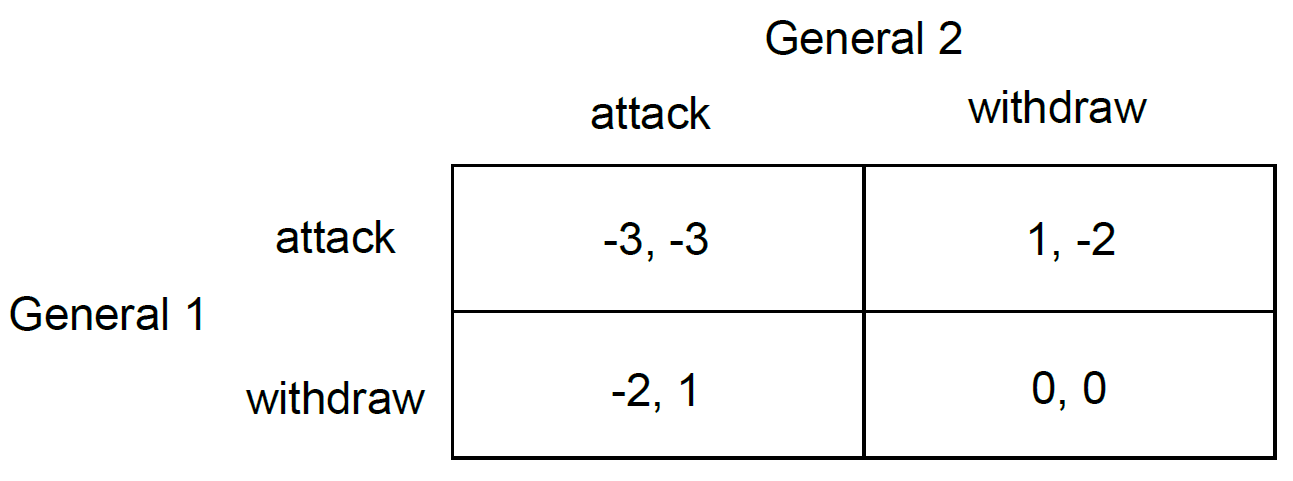
\includegraphics[width=0.4\textwidth]{Pictures/two_generals_GT.png}
\end{figure}

According to Adam Smith: "In competition, individual ambition serve the common
good."

Contrary to this: Nash's key sentence: "The best result comes from everyone in
the group doing what is best for himself \underline{and} the group."

\subsubsection{History}
John von Neumann (1903-1957)
\begin{itemize}
    \item Born in Budapest
    \item Diploma in chemical engineering from ETH (1926)
    \item PhD in mathematics from University of Budapest
    \item Founded the field of game theory as a mathematical discipline
\end{itemize}

Oskar Morgenstern (1902-1977)
\begin{itemize}
    \item Born in Görlitz (Germany)
    \item Student and PhD in political sciences at University of Vienna
    \item Together with Neumann, he founded the mathematical field of game
        theory and its application to economics.
\end{itemize}

John Nash (1928-2015)
\begin{itemize}
    \item Born in Bluefield (USA)
    \item Master in Mathematics from Carnegie Mellon University
    \item PhD in Mathematics from Princeton University
    \item Defined and studied what would later be called the "Nash equilibrium"
        and the "Nash bargaining solution"
    \item Nobel prize 1994; Abel prize 2015
\end{itemize}


\subsubsection{What is Game Theory?}

Roger Myerson:
"Game theory can be defined as the study of mathematical
models of conflict and cooperation between intelligent
rational decision-makers. Game theory provides general
mathematical techniques for analyzing situations in which
two or more individuals make decision that will influence one
another’s welfare. […] Game theory offers insights of
fundamental importance for scholars in all branches of the
social sciences, as well as for practical decision-makers."

\subsection{Individual decision-making (Games with $N=1$)}

\begin{example}[Linear programming: production problem]
\end{example}

\begin{figure}[h]
    \centering
    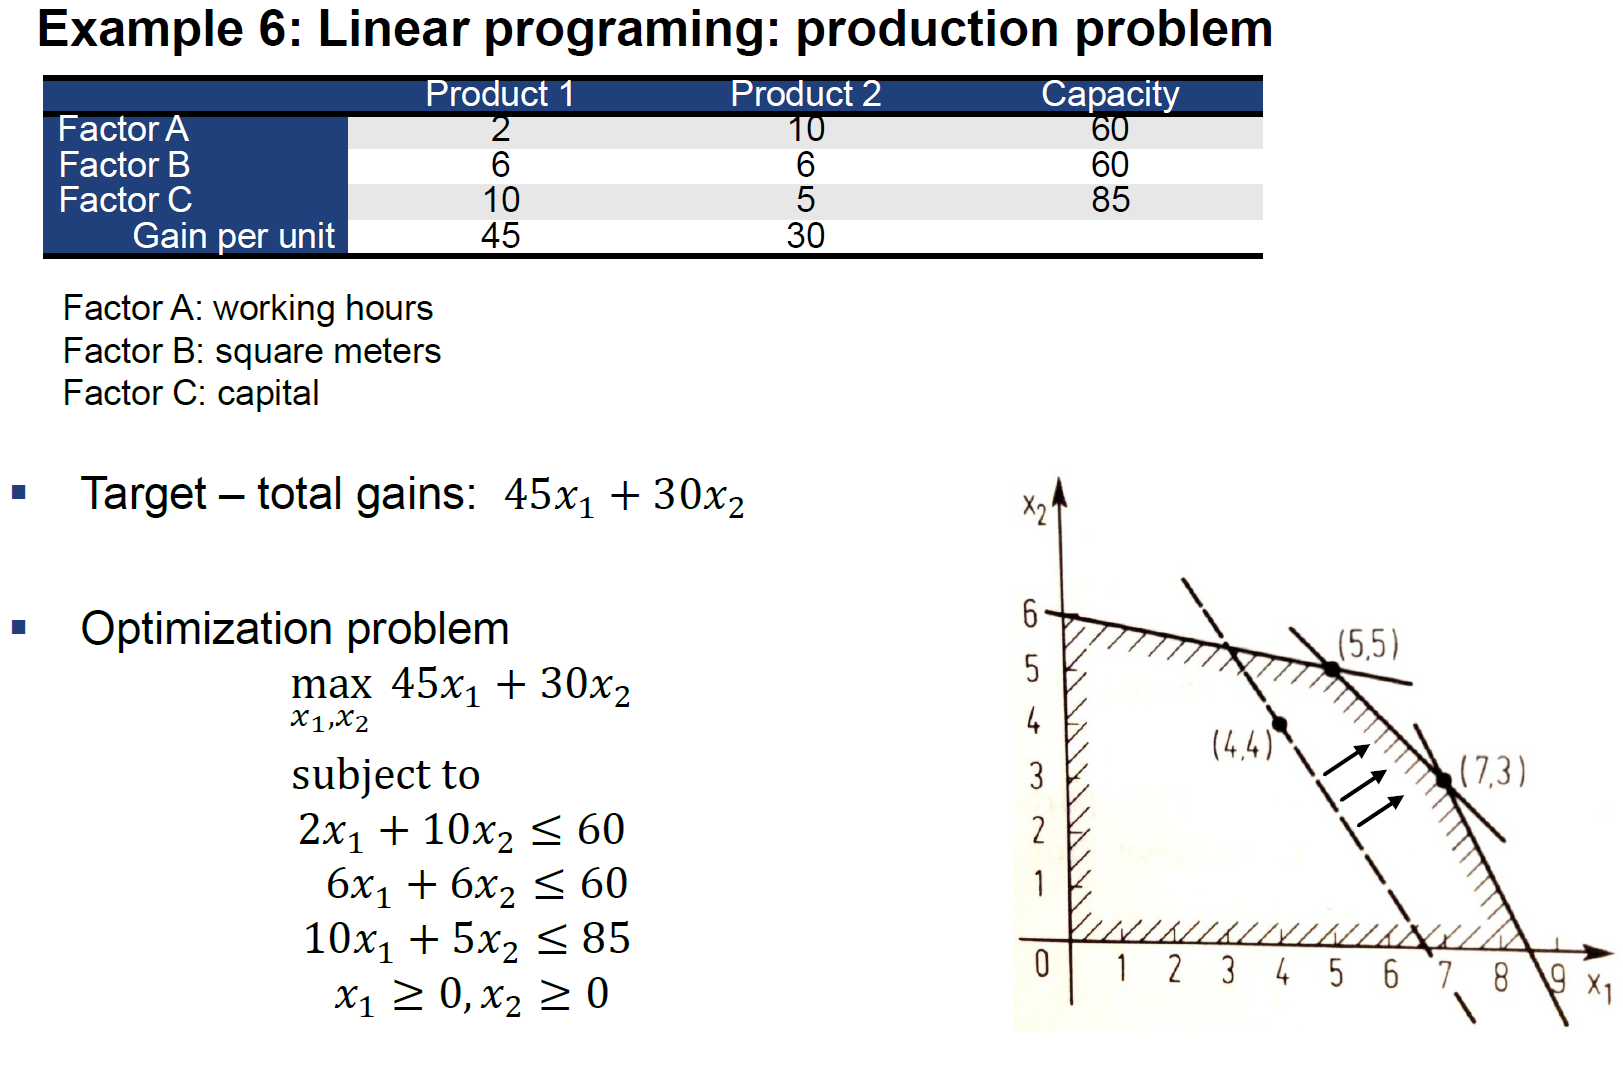
\includegraphics[width=0.45\textwidth]{Pictures/Linear_programming_1.png}
    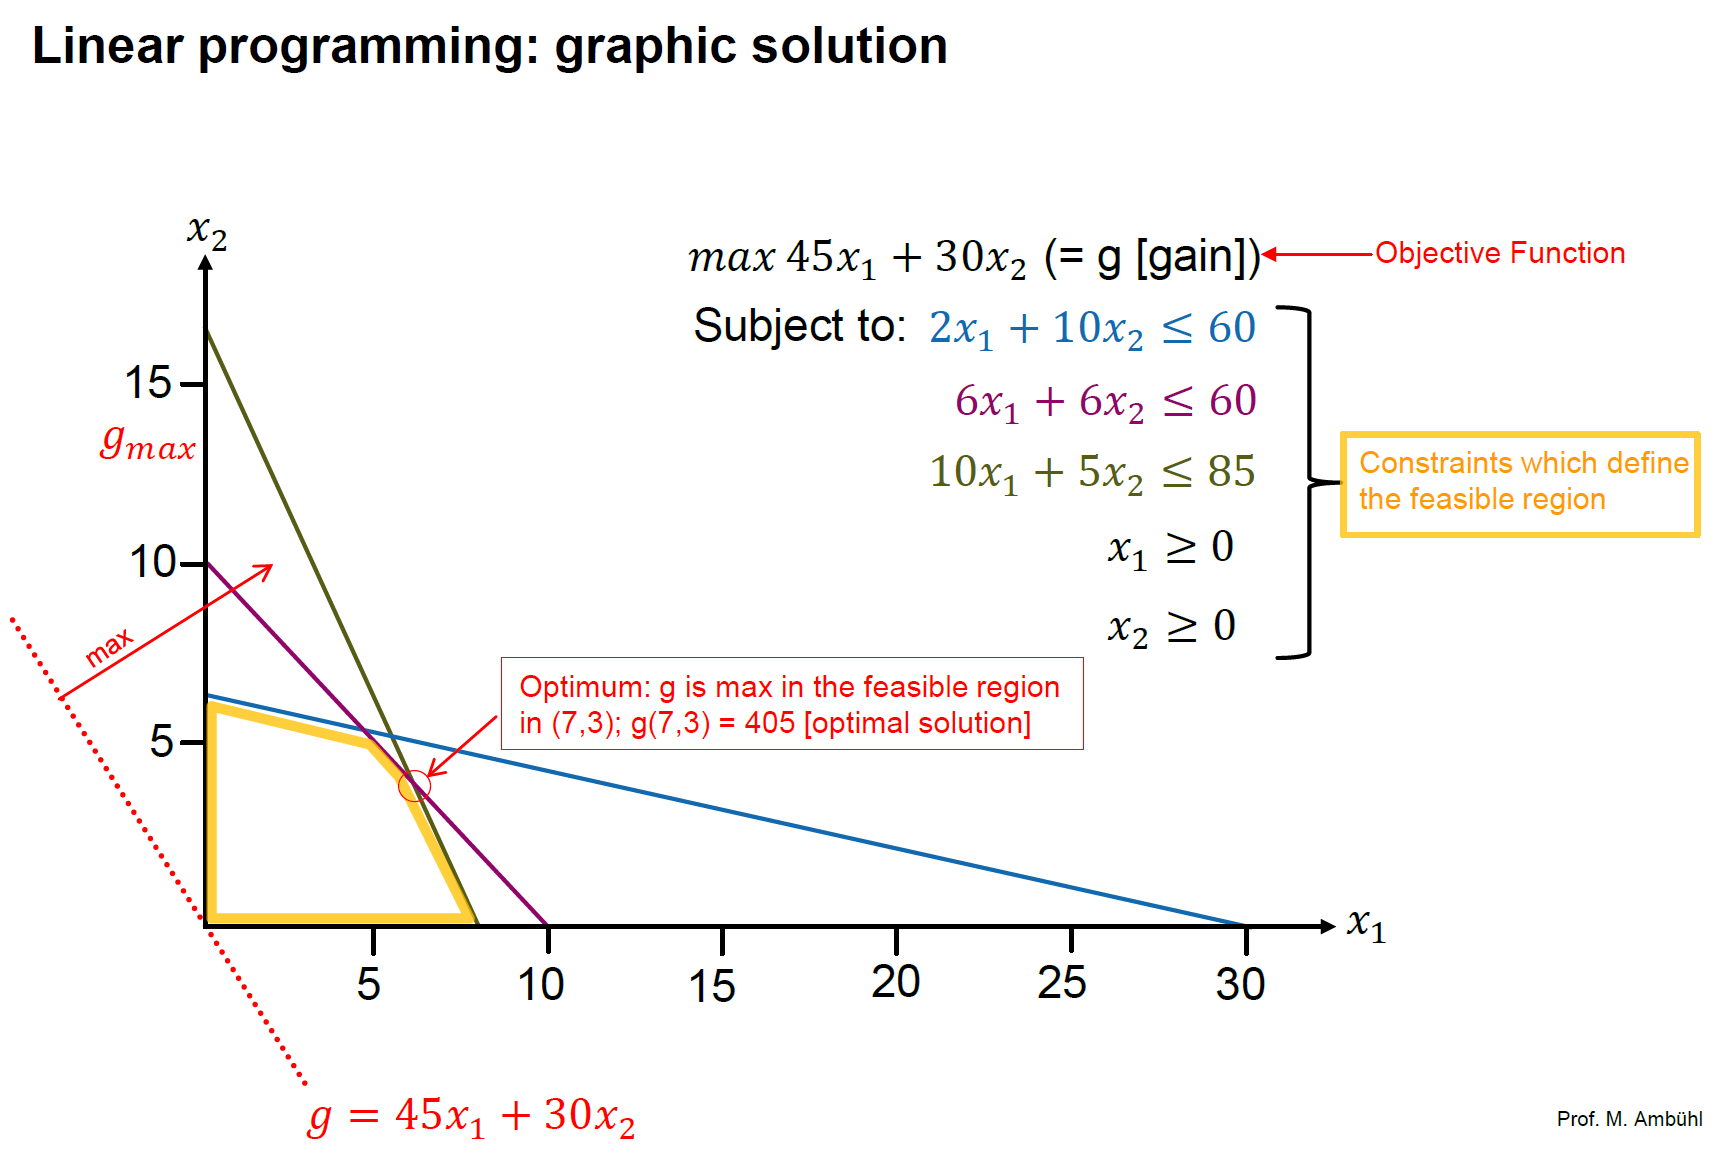
\includegraphics[width=0.45\textwidth]{Pictures/Linear_programming_2.png}
\end{figure}

\begin{example}[Secretary problem]
    There exists different versions of the problem. Here is an easy version:
    \begin{itemize}
        \item There is one secretarial position available
        \item The number of $n$ of applicants is known
        \item The applicants are interviewd sequentially in random order
        \item Each time you see an applicant you have to decide if you take him/her
            or not. The rejection of an applicant cannot be revoked later on. If
            you decide on taking one applicant you can not see any other applicant
            thereafter.
        \item You compare each candidate with the ones you have already seen
        \item $\Rightarrow$ How should you proceed in order to maximize the probablity
            of selecting the \underline{best} candidate?
        \item You should let $\frac{n}{e}$ applicants go by and then select the first
            one whose value exceeds those of all the earlier rejected ones. The probablity
            of getting the best one with this strategy is $\frac{1}{e} \approx 37\%$
        \item Proof:
            \begin{itemize}
                \item $n$ applicants ($n$ is known) are to be presented in a randomized
                    Sequential order
                \item When an applicant is in front of you, you must either chose him,
                    and the game is over, or you reject him, and you can't go back.
                \item The probablity to choose the best is at each stage $\frac{1}{n}$.
                \item Suppose you reject the first candidate, then there is a $\frac{1}{n}$
                    chance that this one was the best and you failed to select the best
                \item The second now presents himself and you compare him to the first. If
                    he is not as good as the first you will obviously not select him; but
                    even if the second is better than the first, you might still want to pass
                    up on that person because you think the best is among the remaining ones
                \item The best of the rejected ones serves you as the standard for judging
                    the ones to come. So the best of the first $x$ ($x$: rejected ones) will
                    represent a standard against which to judge the remainder.
                \item How many should you let go before making your choice? What chance do you
                    have to pick the best?
                    \begin{itemize}
                        \item \underline{Strategy S}: Idea: Divide the universal sequence of
                            all candidates into two groups; the first group (called the rejected
                            ones or the “standard-setting group”) consisting of a proportion $t$
                            of candidates, is used only toidentify the best in that group; we then
                            sequentially observe the candidates in the second group (called the
                            selection group)and choose the first who beats the best in the
                            standard-setting group. $P(t)$:Probability of finding the best
                            candidate when the standard-setting group comprises a proportion
                            of t candidates. This stragegy will result in the choice of the best, if
                            \begin{itemize}
                                \item the second best falls in the first group (proportion $t$,
                                    $0 \leq t \leq 1$) and the first best in the second
                                    (proportion $(1-t)$). This has the probability $p = t (1-t)$.
                                \item the third best falls in the first group (probability $p=t$)
                                    and the first best in the second group ($p = (1-t)$) and the second
                                    best also in the second group ($p=(1-t)$), and the first comes
                                    before the second ($p=\frac{1}{2}$). This has probability of
                                    $p = t \frac{(1-t)^2}{2}$.
                                \item the fourth best falls in the first segment and the first,
                                    second, and third best in the second segment and the first comes
                                    before the second or the third: $p = \frac{t (1-t)^3}{3}$
                                \item and so on\dots
                                \item Hence: $P(t) = t (1-t) + \frac{t(1-t)^2}{2} + \frac{t (1-t)^3}{3} + \dots$ assuming $n \rightarrow \infty$:
                                    $P(t) = t \eckigeklammer{(1-t) + \frac{(1-t)^2}{2} + \frac{(1-t)^3}{3} + \dots}
                                            = - t \ln(t)$
                                \item To find the optimal proportion for the standard-setting
                                    group, we differentiate $P(t)$ and set $P'(t)$ to $0$. This
                                    yields: $t = \frac{1}{e}$, so $P\klammer{\frac{1}{e}} = \frac{1}{e}$
                            \end{itemize}
                    \end{itemize}
            \end{itemize}
        \item Concrete Case, $n$ small ($n=4$):
            \begin{itemize}
                \item You want to select the best candidate, only the best
                \item Random order, each order being equally likely
                \item You can rank all applicants from worst to best; the
                    decision to accept or reject is based only on the relative
                    rank
                \item Let $n=4$
                \item Best candidate: rank 4; least best candidate: rank 1
                \item Ranks are ordinal numbers
                \item $n!$ permutationspossible, i.e. $4 \cdot 3 \cdot 2 \cdot 1=24$
                \item Strategy: Let $t$ ($0 \leq t < 4$) applicants pass by, then
                    select the first one that is better than the rejected one(s)
                \item $\frac{4}{e} \approx 1.471$, rounded: $t=1$.
            \end{itemize}
    \end{itemize}
\end{example}

\begin{figure}[h]
    \centering
    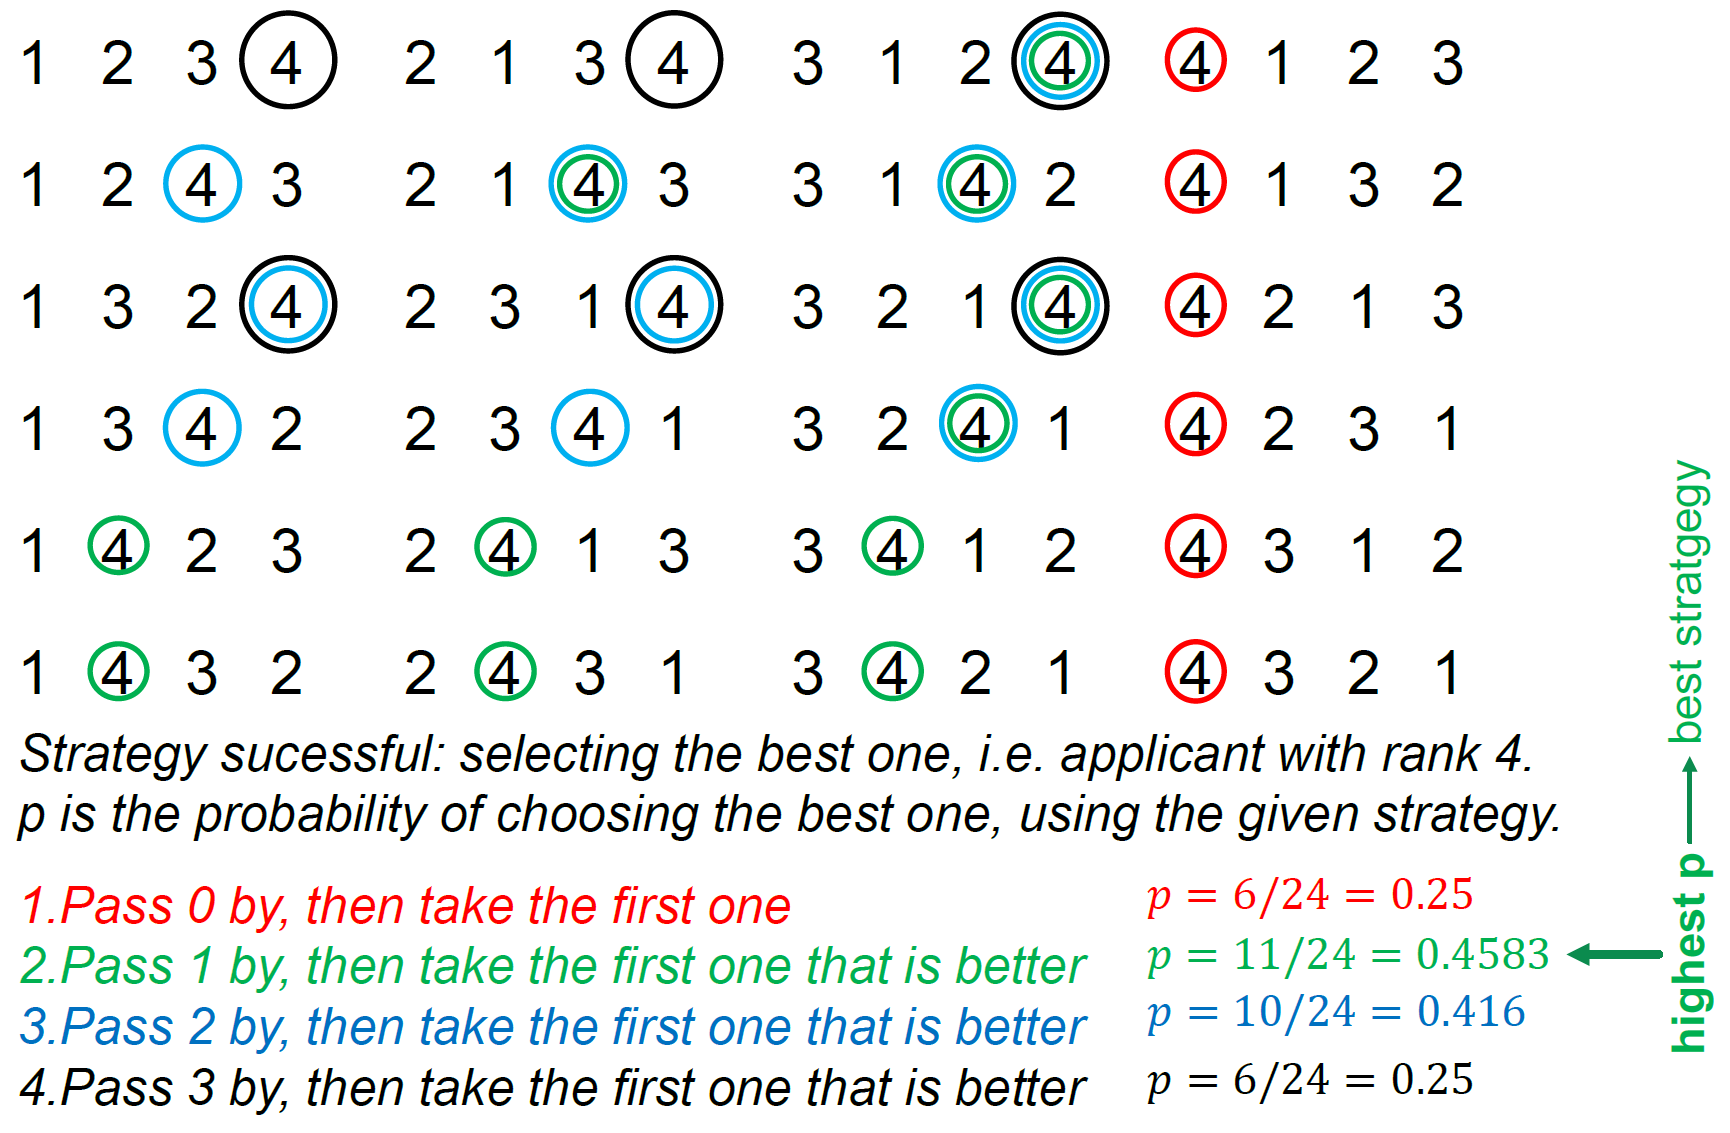
\includegraphics[width=0.35\textwidth]{Pictures/secretary_problem_n_4.png}
\end{figure}

\begin{minipage}{0.45\textwidth}
    \paragraph{Example $8$: Casino (Game against nature)}
    \begin{itemize}
        \item You have four actions: A, B, C, and D
        \item Choices of nature: W, X, Y, and Z
    \end{itemize}
\end{minipage}
\begin{minipage}{0.45\textwidth}
    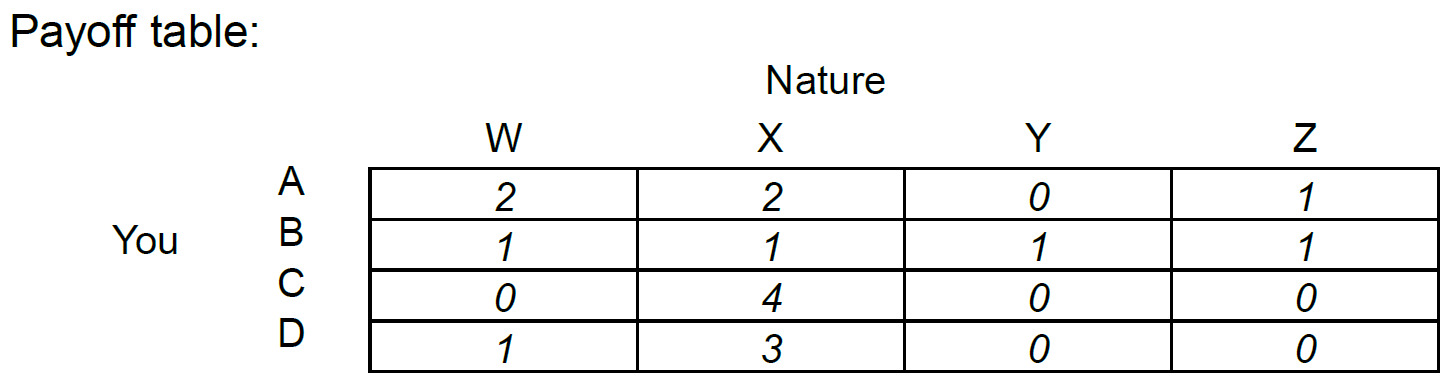
\includegraphics[width=0.9\textwidth]{Pictures/Payoff_table.png}
\end{minipage}

\begin{figure}[H]
    \centering
    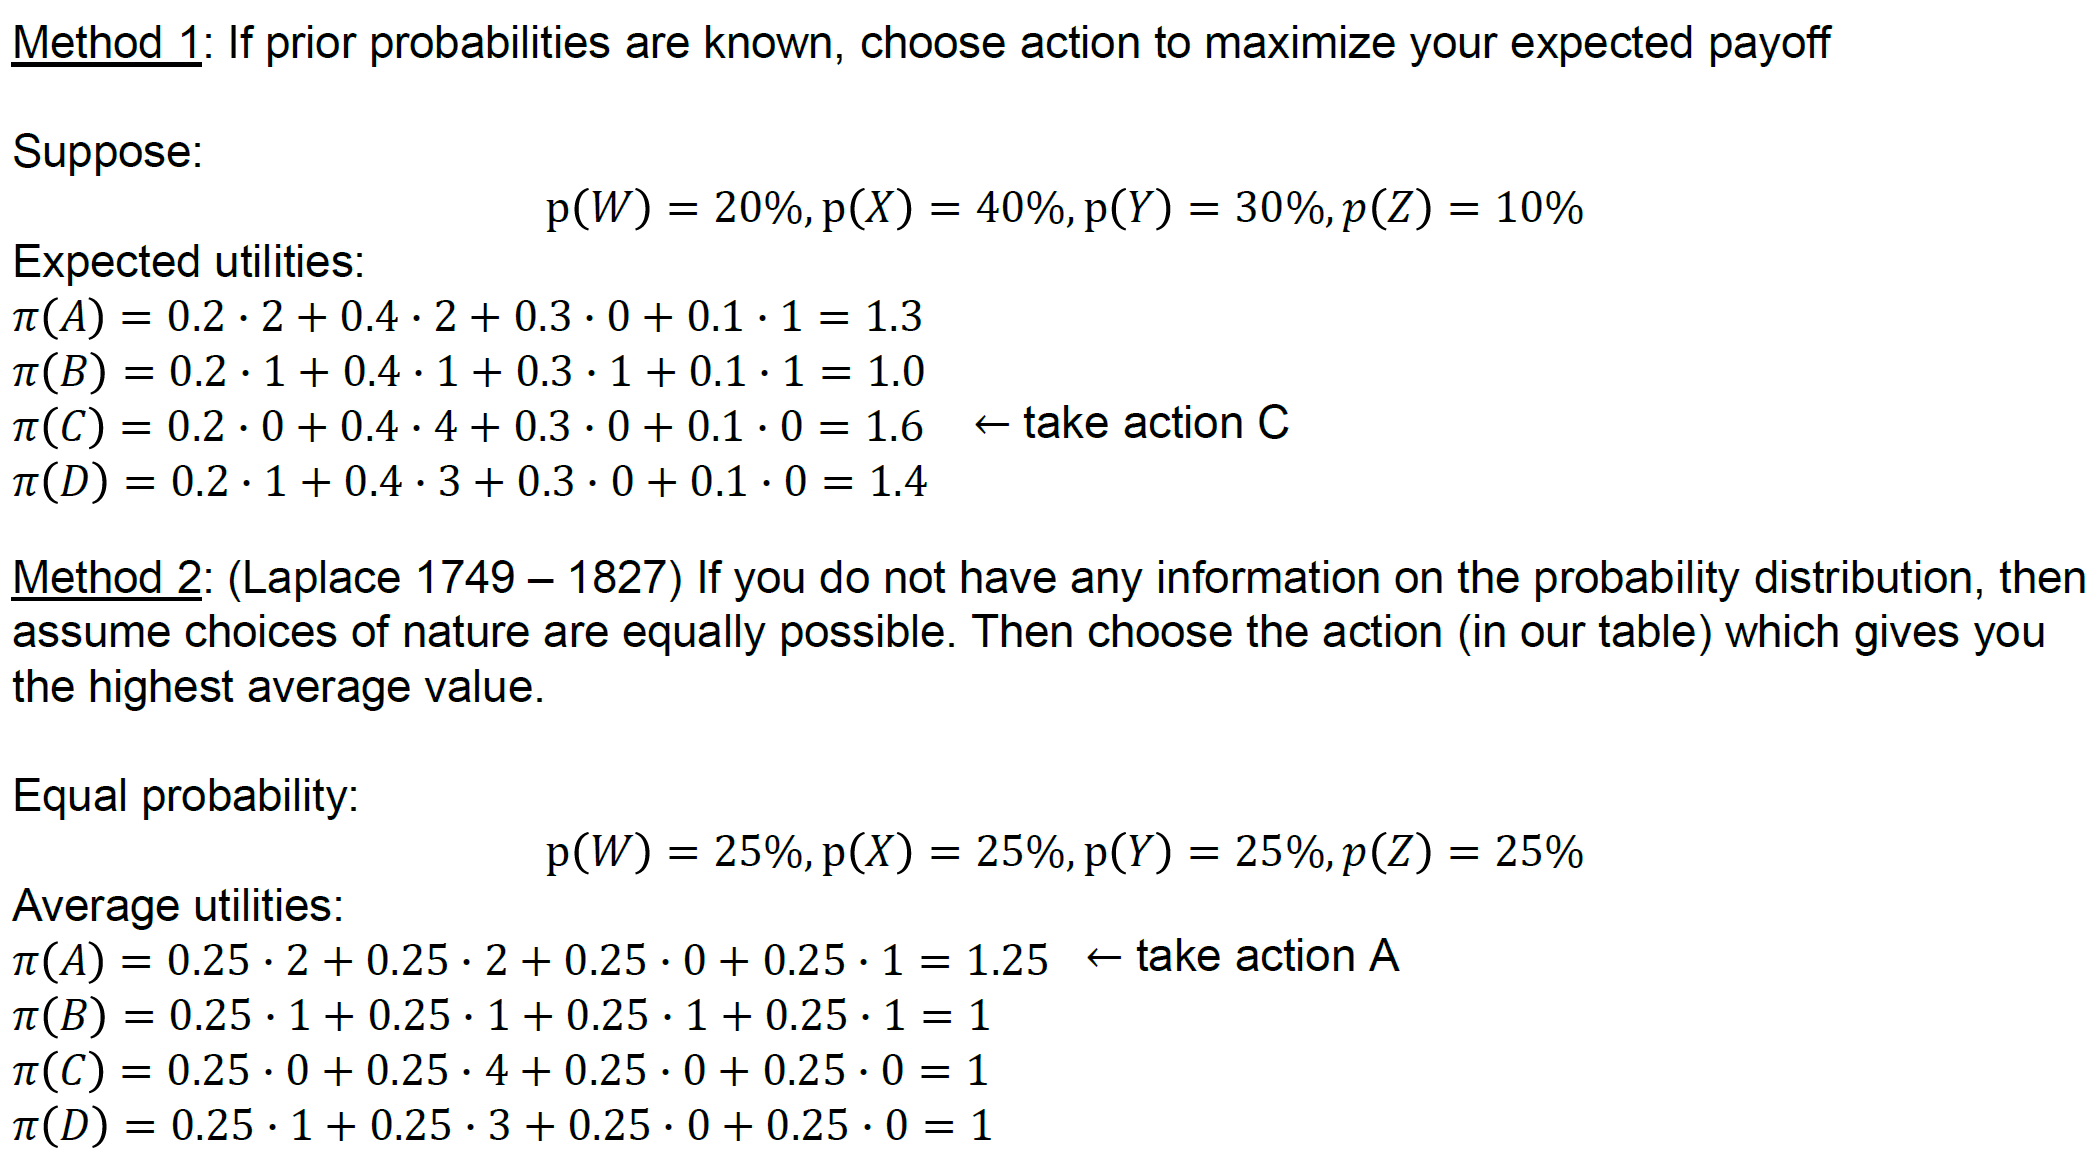
\includegraphics[width=0.6\textwidth]{Pictures/method_1_and_2.png}
    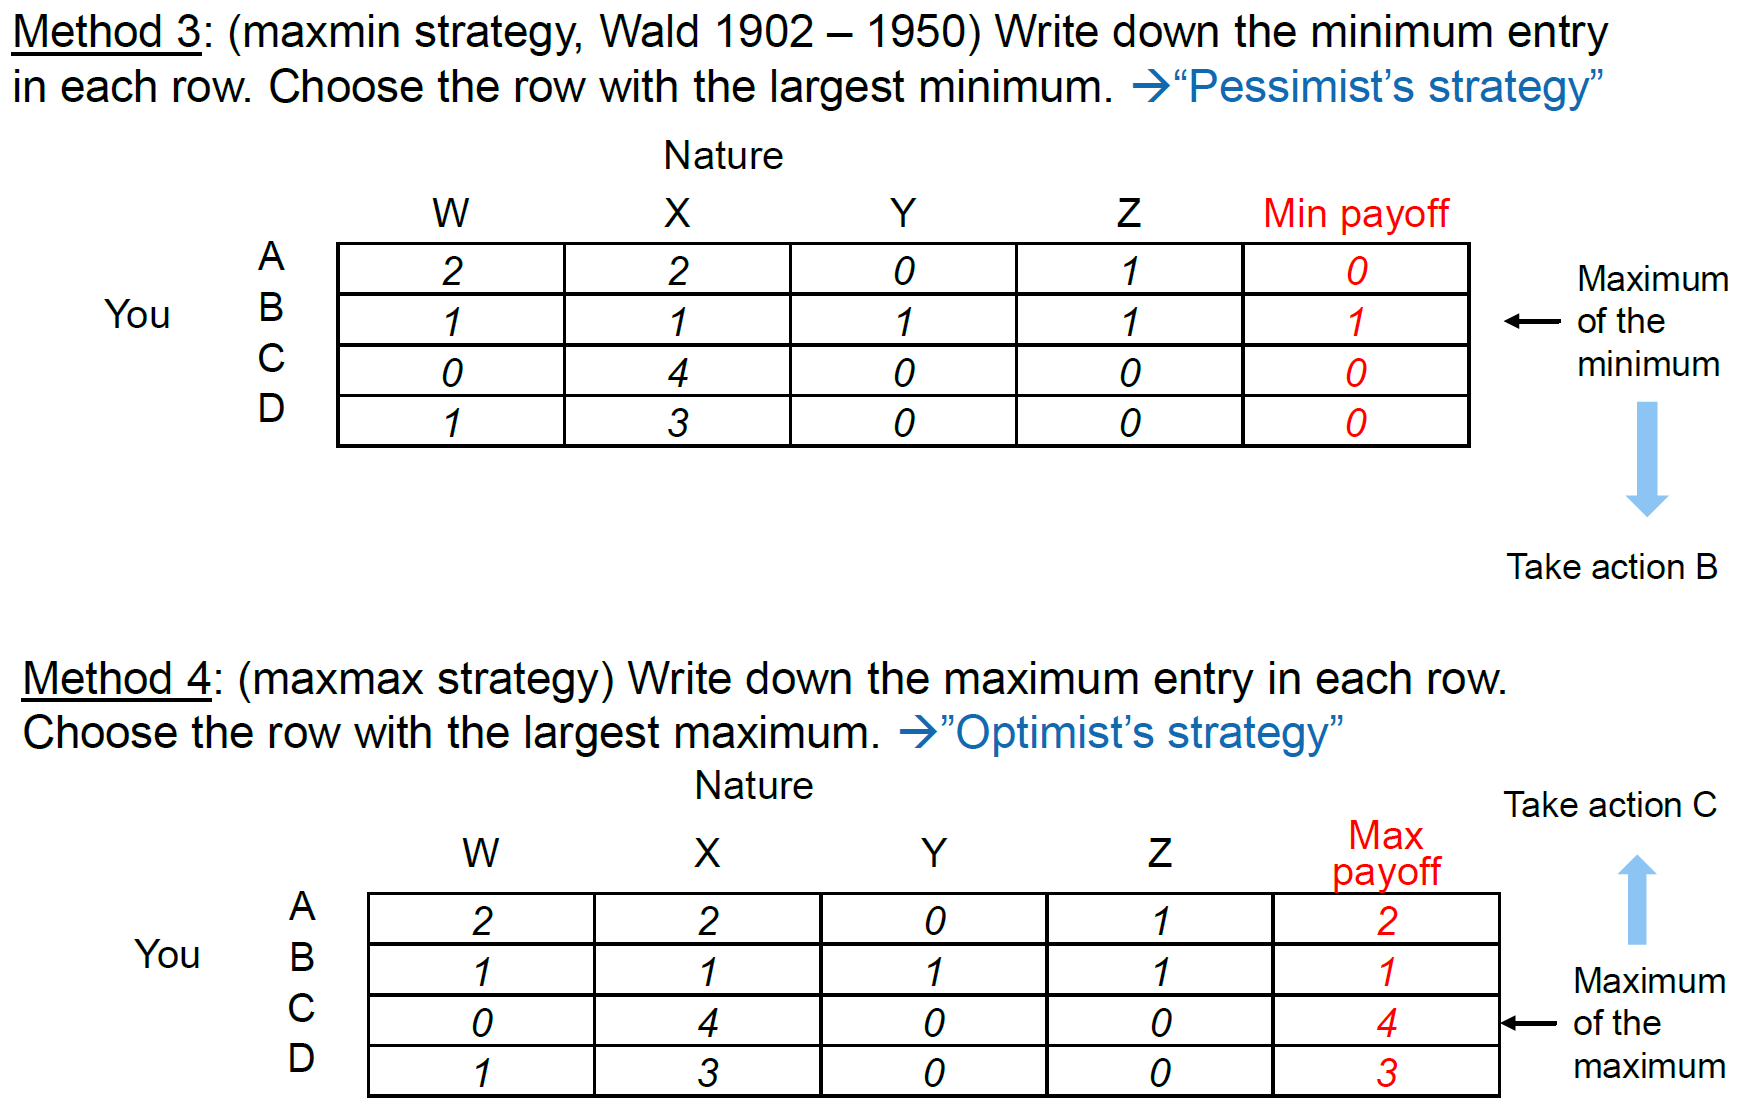
\includegraphics[width=0.6\textwidth]{Pictures/Method_3_and_4.png}
    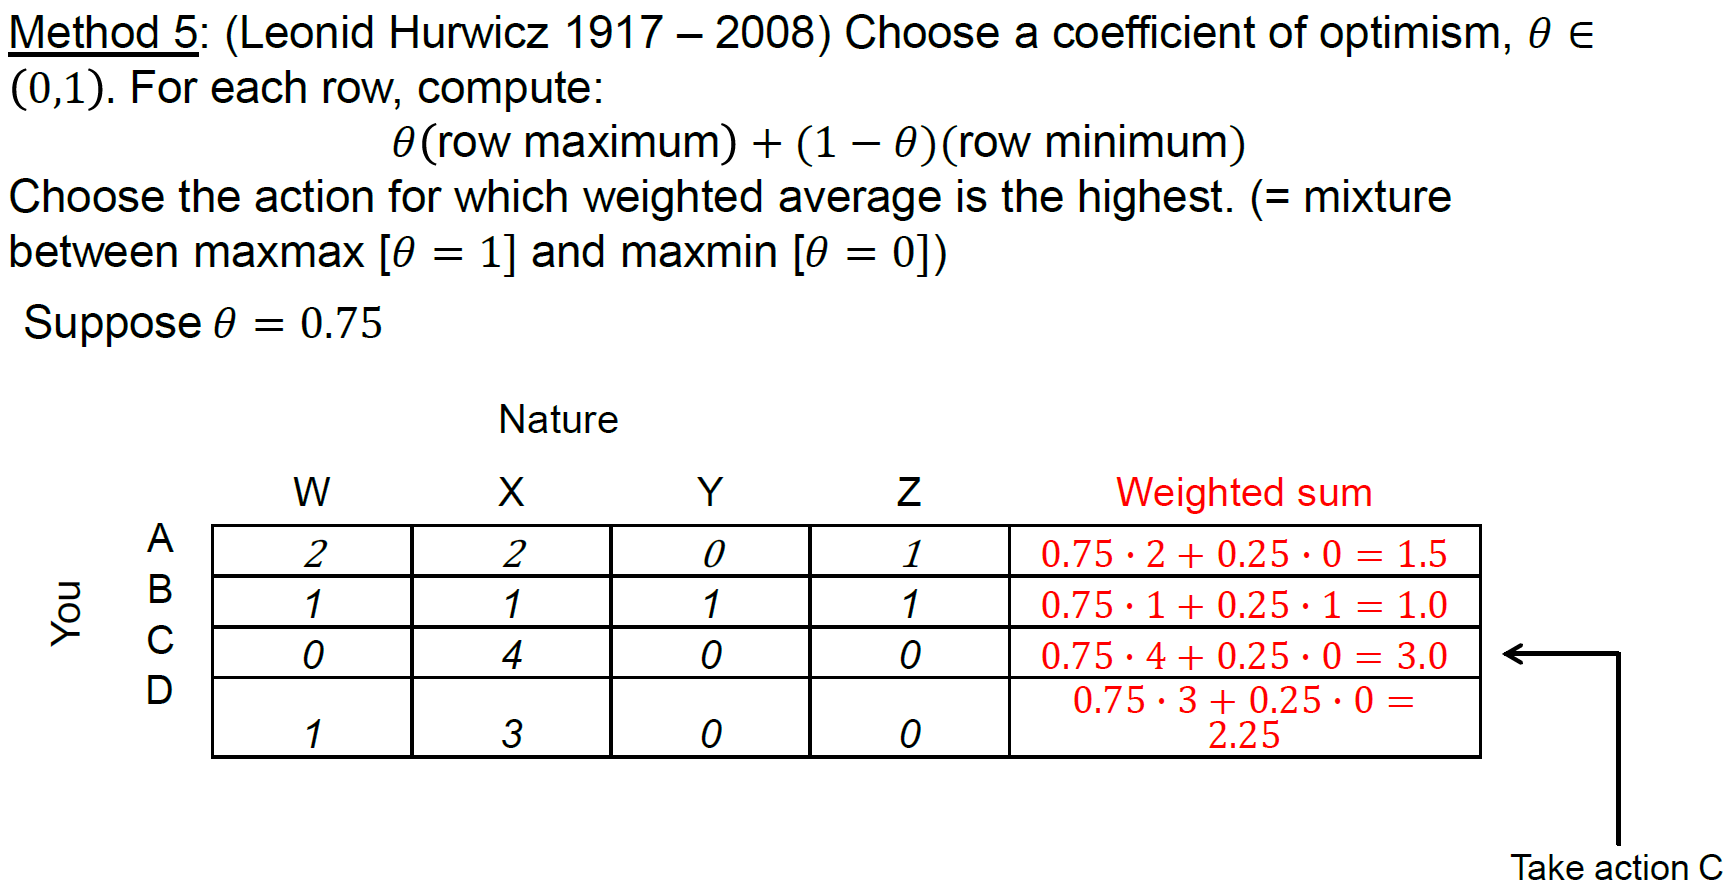
\includegraphics[width=0.6\textwidth]{Pictures/method_5.png}
    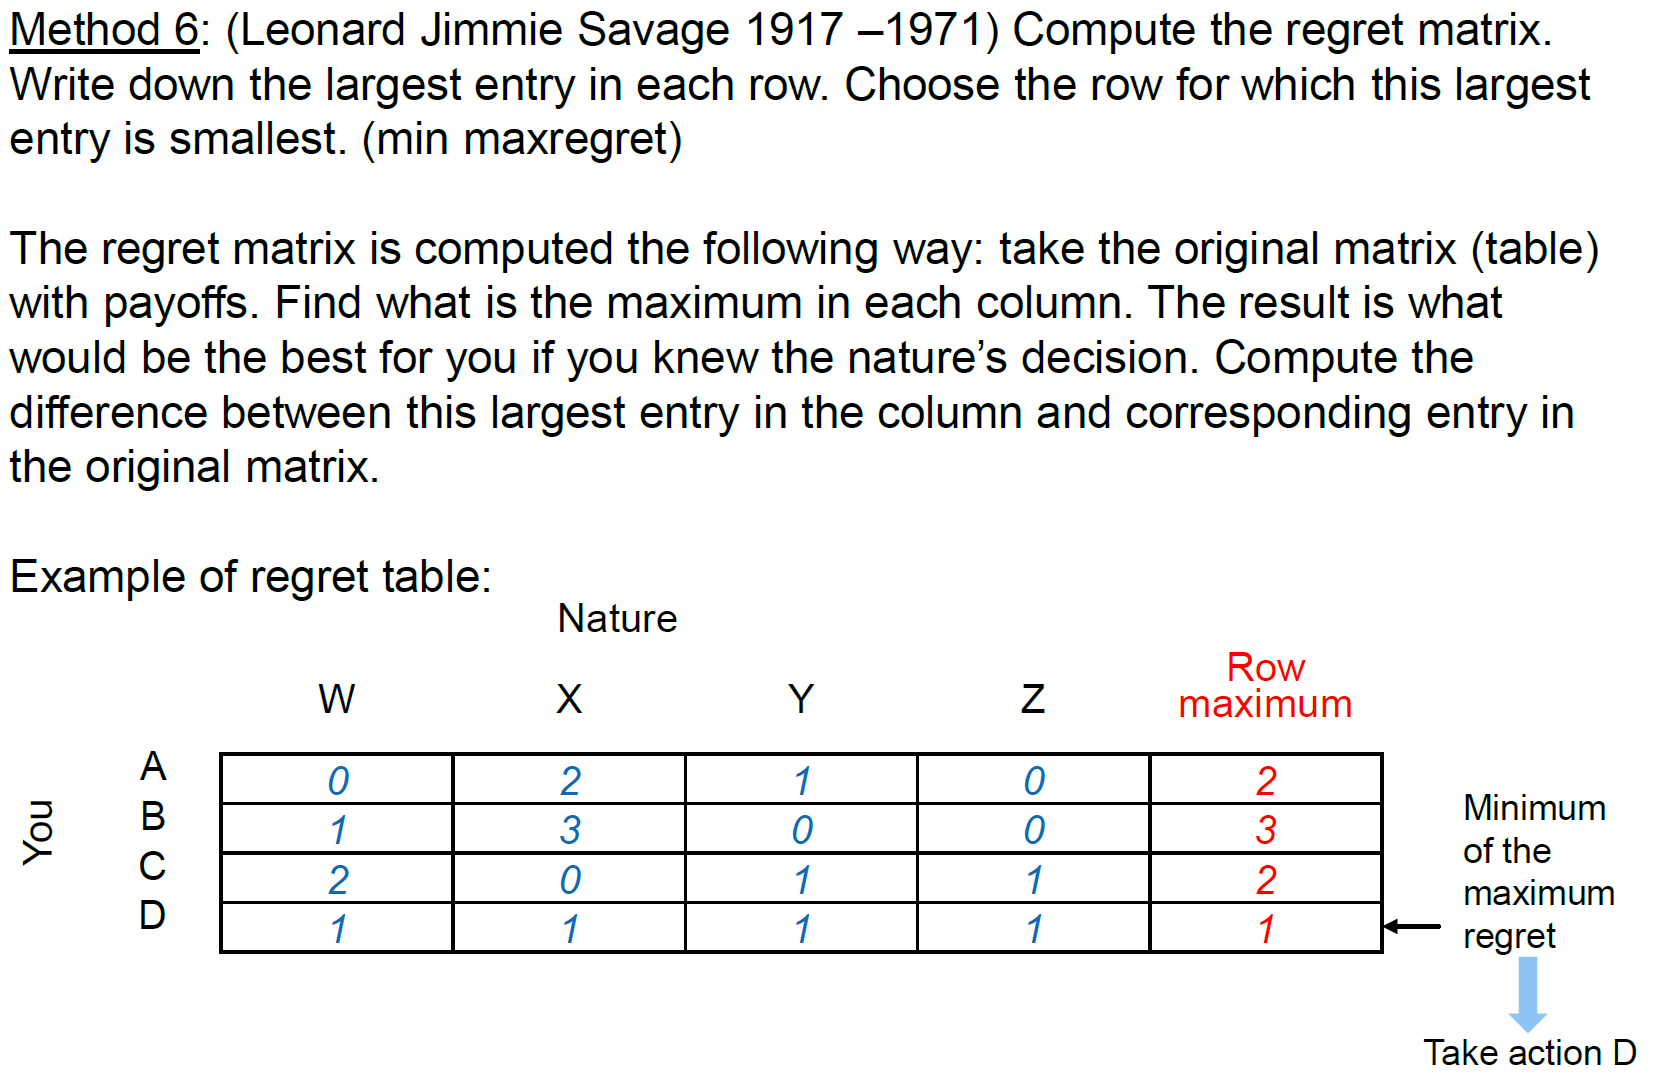
\includegraphics[width=0.6\textwidth]{Pictures/method_6.png}
\end{figure}

\begin{figure}[H]
    \centering
    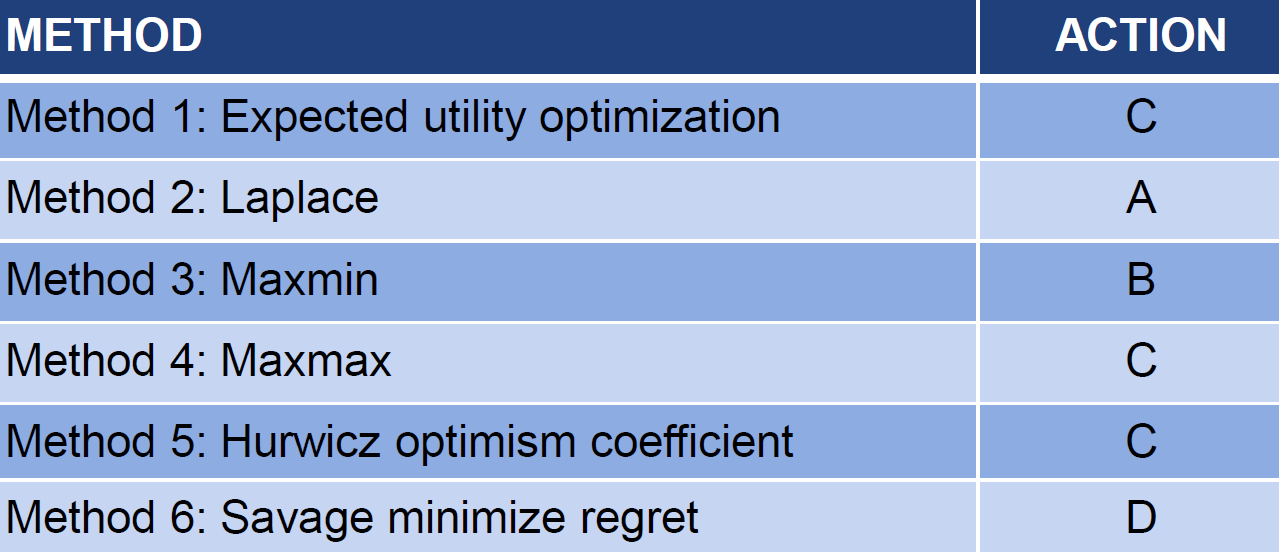
\includegraphics[width=0.5\textwidth]{Pictures/results_method.png}
\end{figure}

\subsection{Group of $N$ individuals (Game with $N>1$)}

\subsubsection{Non cooperative Games}

\paragraph{Static Games}

\begin{itemize}
    \item The Players:
        Who is involved?
    \item The rules:
        \begin{itemize}
            \item Who moves when?
            \item What do they know when they move?
            \item What can they do?
        \end{itemize}
    \item The outcomes: For each possible set of actions by the players what
        is the outcome of the game?
    \item The payoffs: What are the players' preferences (i.e. utilities) over
        the possible outcomes?
    \item Pure strategies - there is no randomization when players take an action.
\end{itemize}

\subparagraph{Constant sum Game}

Pure Strategy:

Example 9: Boris and Sophie divide the surplus

\begin{enumerate}[a)]
    \item Situation in words
        \begin{itemize}
            \item Imagine Sophie and Boris decide to finalize a price in the following manner:
            \item They sit in different rooms, don’t communicate with each other and announce their decision simultaneously: A or B
            \item If both announce A they trade without concessions (i.e. each gets zero additional surplus)
            \item If Boris announces B and Sophie –A : The price will shift towards Sophie by CHF 5
            \item If Boris announces A and Sophie –B: The price will shift towards Boris by CHF 4
            \item If both announce B: Sophie will make a concession towards Boris by CHF 1
        \end{itemize}
    \item Game
        \begin{enumerate}[(i)]
            \item Players: 2 (Boris, Sophie)
            \item Actions: 2 (A,B)
            \item Preferences: Boris: $(A,B) \succ (B,B) \succ (A,A) \succ (B,A)$,
                Sophie: $(A,B) \prec (B,B) \prec (A,A) \prec (B,A)$
            \item Payoffs are presented in the normal form below
            
                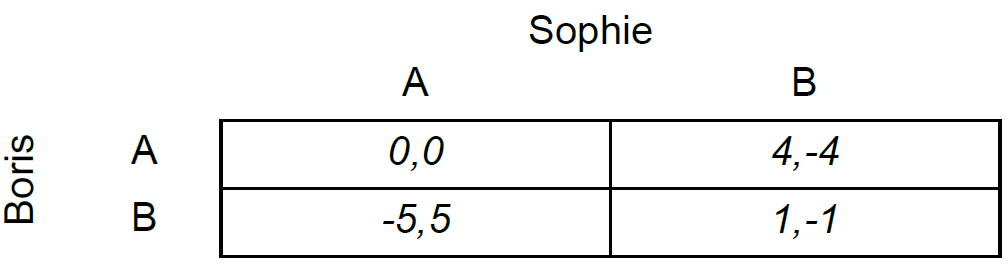
\includegraphics[width=0.4\textwidth]{Pictures/boris_sophie_game.png}
            \item Zero sum Game.
        \end{enumerate}
\end{enumerate}

\begin{figure}[H]
    \centering
    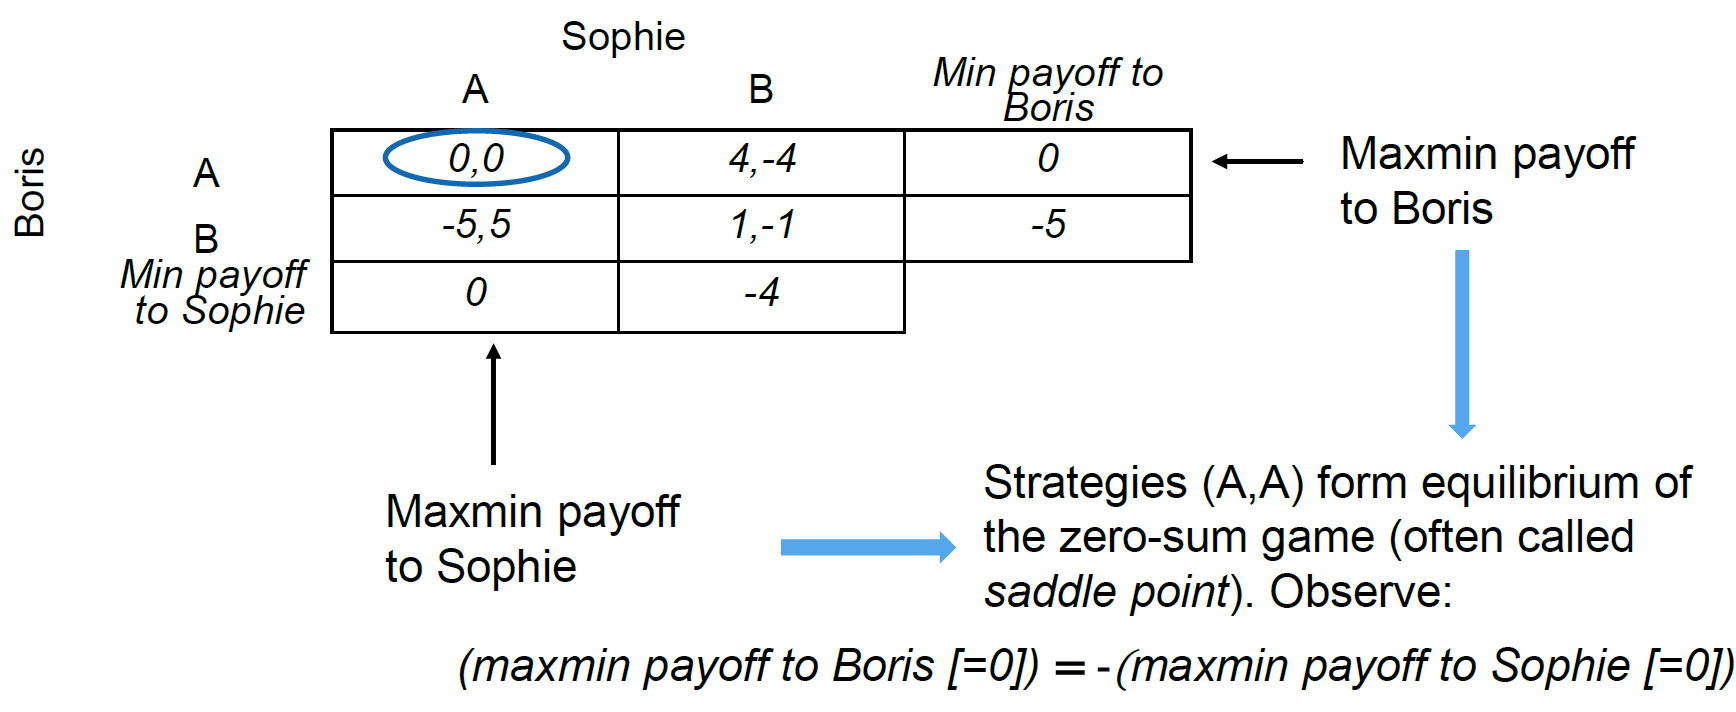
\includegraphics[width=0.5\textwidth]{Pictures/maxim_analysis_saddle_point.png}
\end{figure}

\begin{figure}[H]
    \centering
    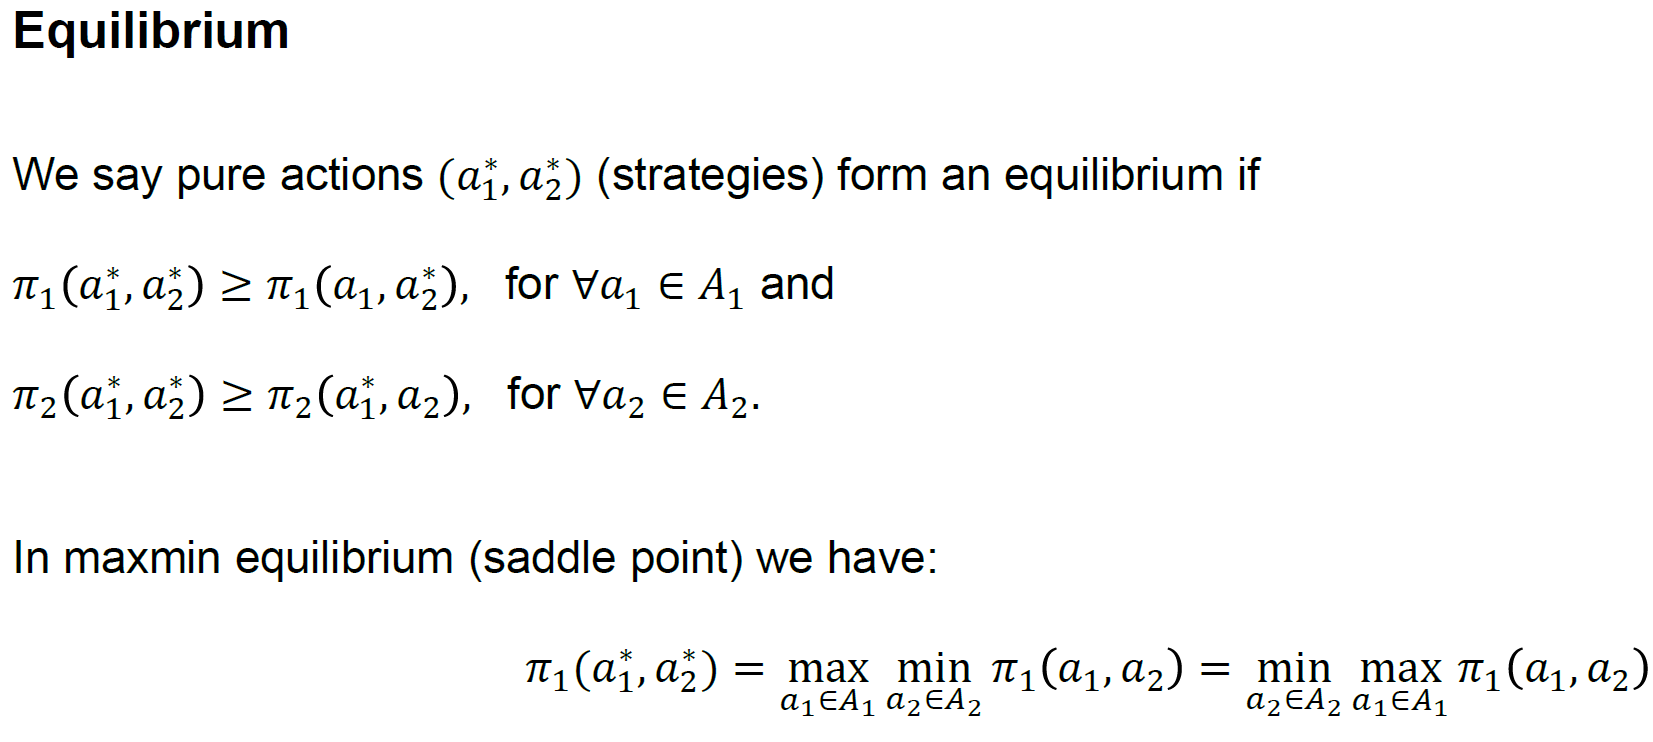
\includegraphics[width=0.5\textwidth]{Pictures/equilibrium.png}
\end{figure}

\begin{theorem}[Maxmin (John von Neumann)]    
\end{theorem}

\begin{figure}[H]
    \centering
    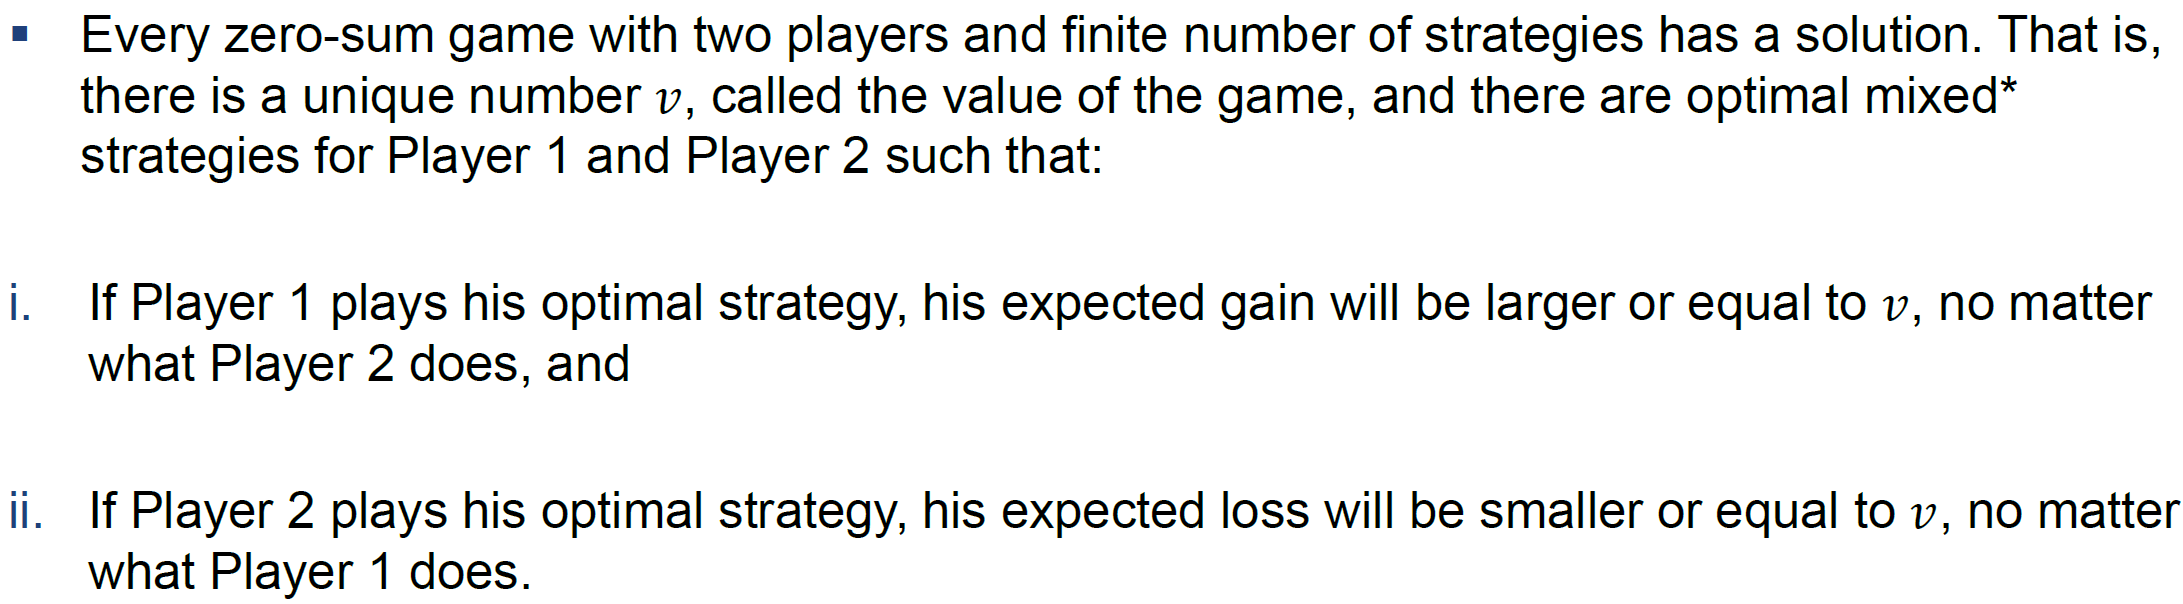
\includegraphics[width=0.5\textwidth]{Pictures/maxmin_theorem.png}
\end{figure}

Comments:
\begin{itemize}
    \item Game Theory began with studies of zero-sum games
    \item In zero-sum (also called constant sum) games:
        \begin{itemize}
            \item The sum of payoffs in each cell is zero (or constant)
            \item The interests of the players are strictly opposite
        \end{itemize}
    \item Maxmin strategy enables a player to calculate the maximum of the minimum
        payoff he can achieve. This strategy guarantees him a security level -
        the minimum payoff for a player, when he plays non-cooperative.
\end{itemize}

Example 10: 2 players, 4 strategies:

\begin{figure}[H]
    \centering
    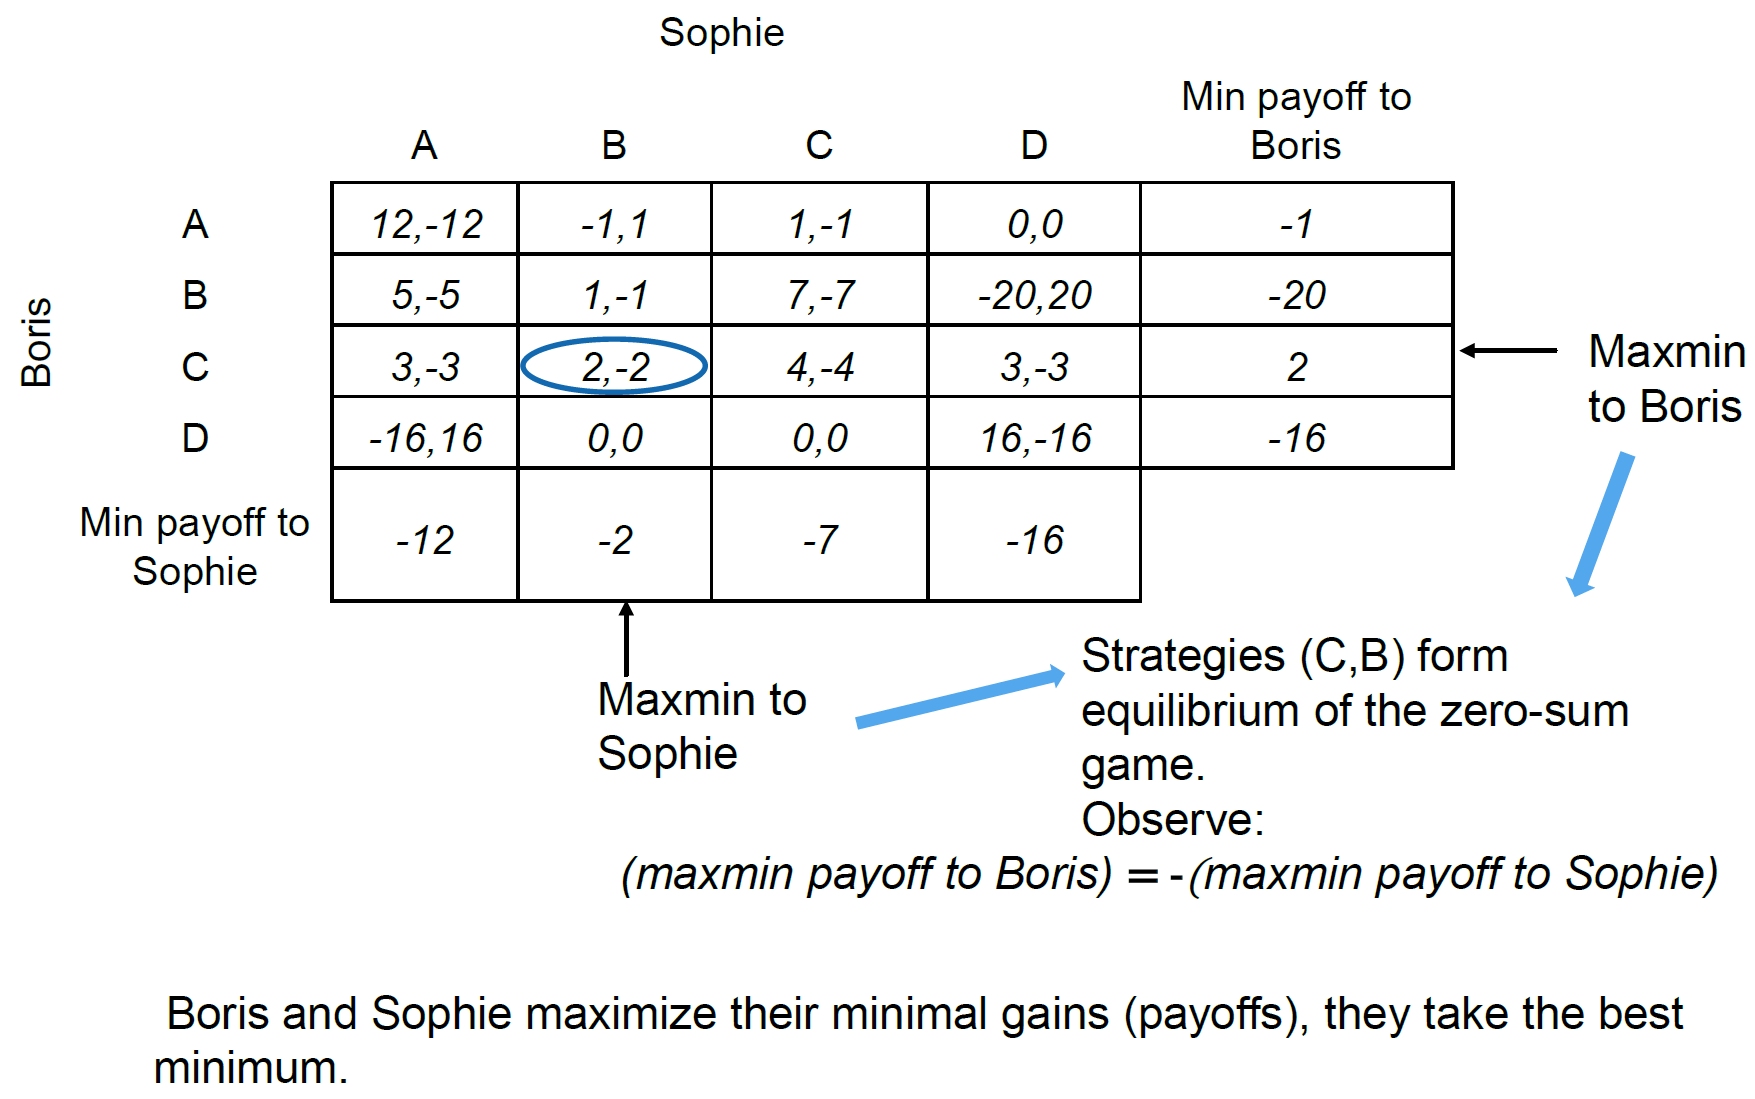
\includegraphics[width=0.5\textwidth]{Pictures/example_10.png}
    \caption{Solution with maxmin}
\end{figure}

\begin{figure}[H]
    \centering
    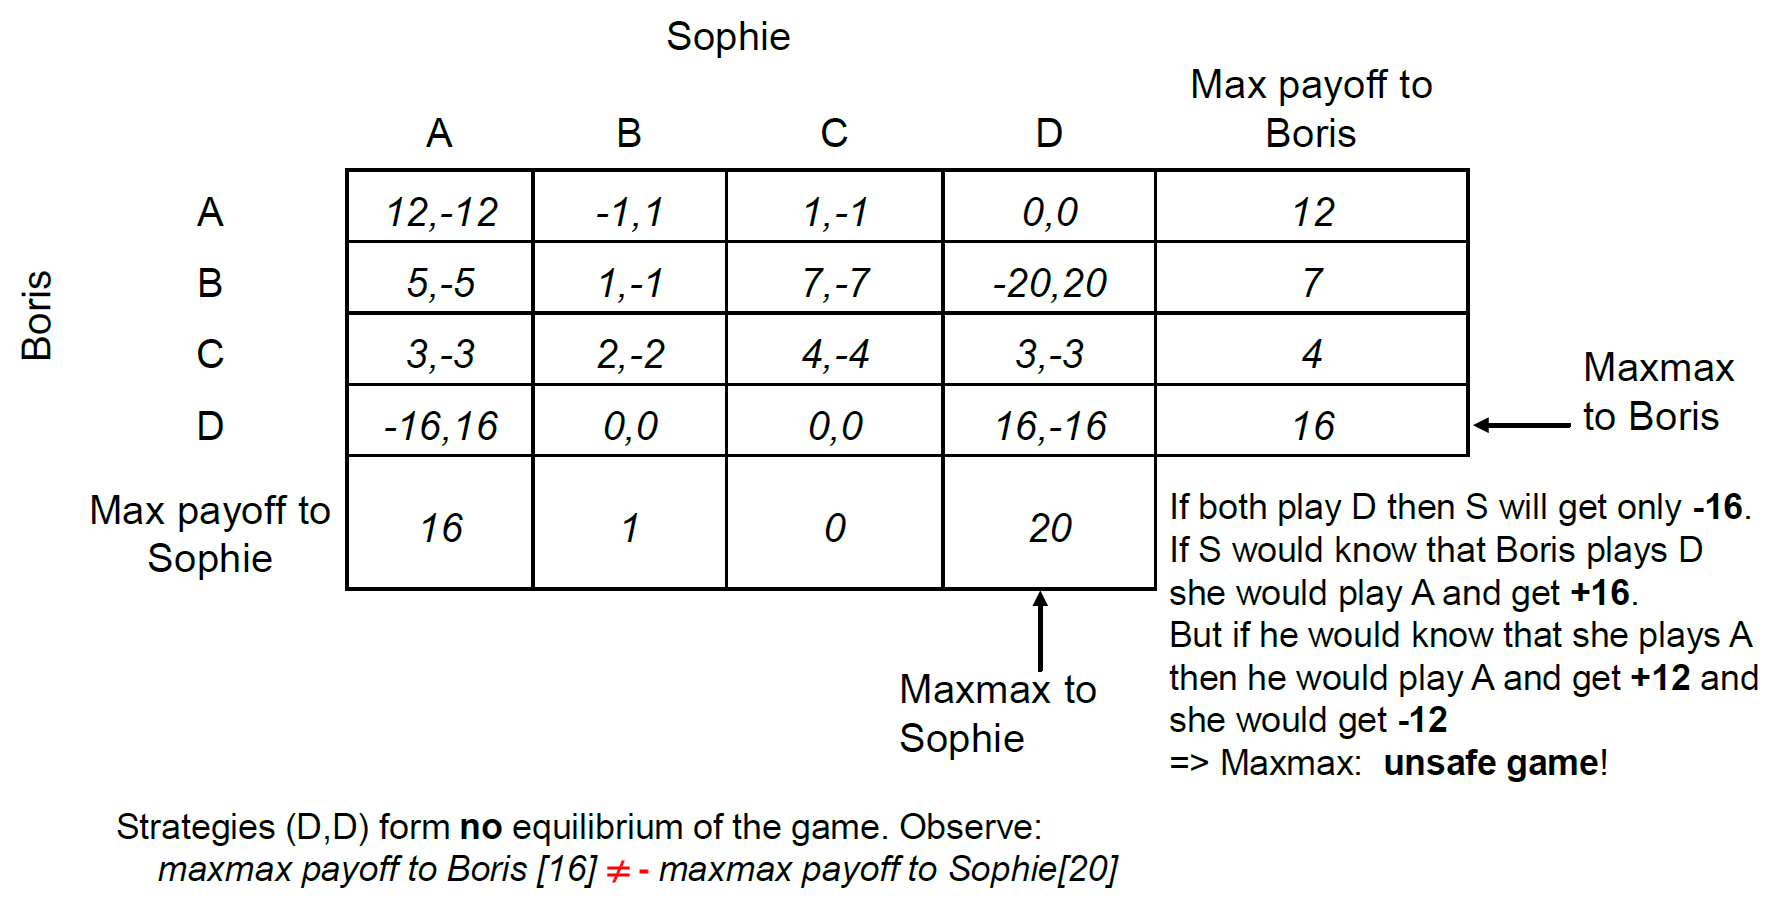
\includegraphics[width=0.5\textwidth]{Pictures/example_10_maxmax.png}
    \caption{Solution with maxmax}
\end{figure}

\begin{figure}[H]
    \centering
    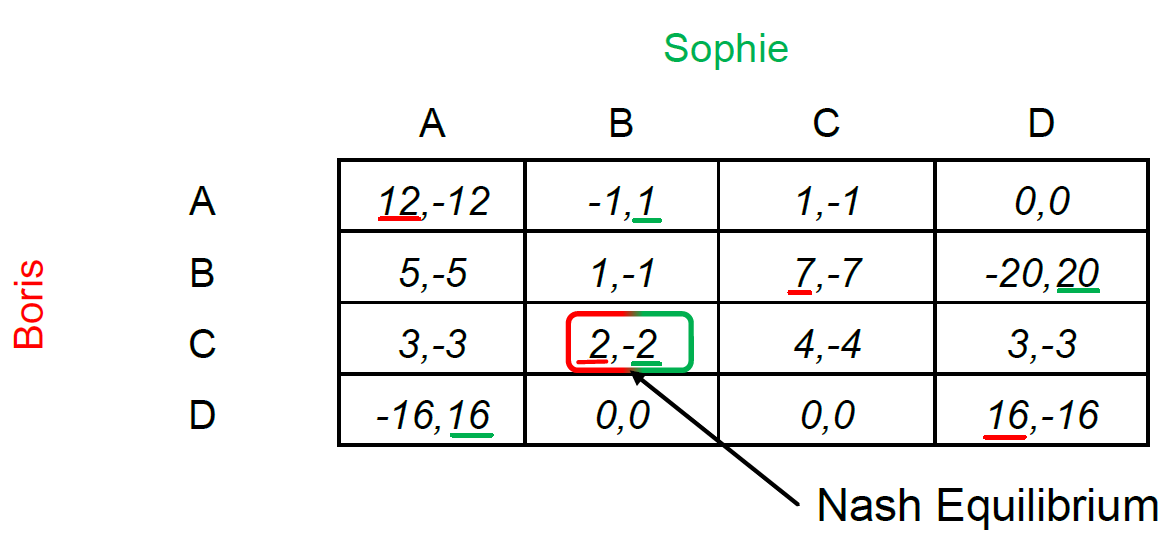
\includegraphics[width=0.5\textwidth]{Pictures/example_10_best_response.png}
    \caption{Solution with the best response / Nash equilibrium}
\end{figure}

\underline{Nash Equilibrium}

\begin{figure}[H]
    \centering
    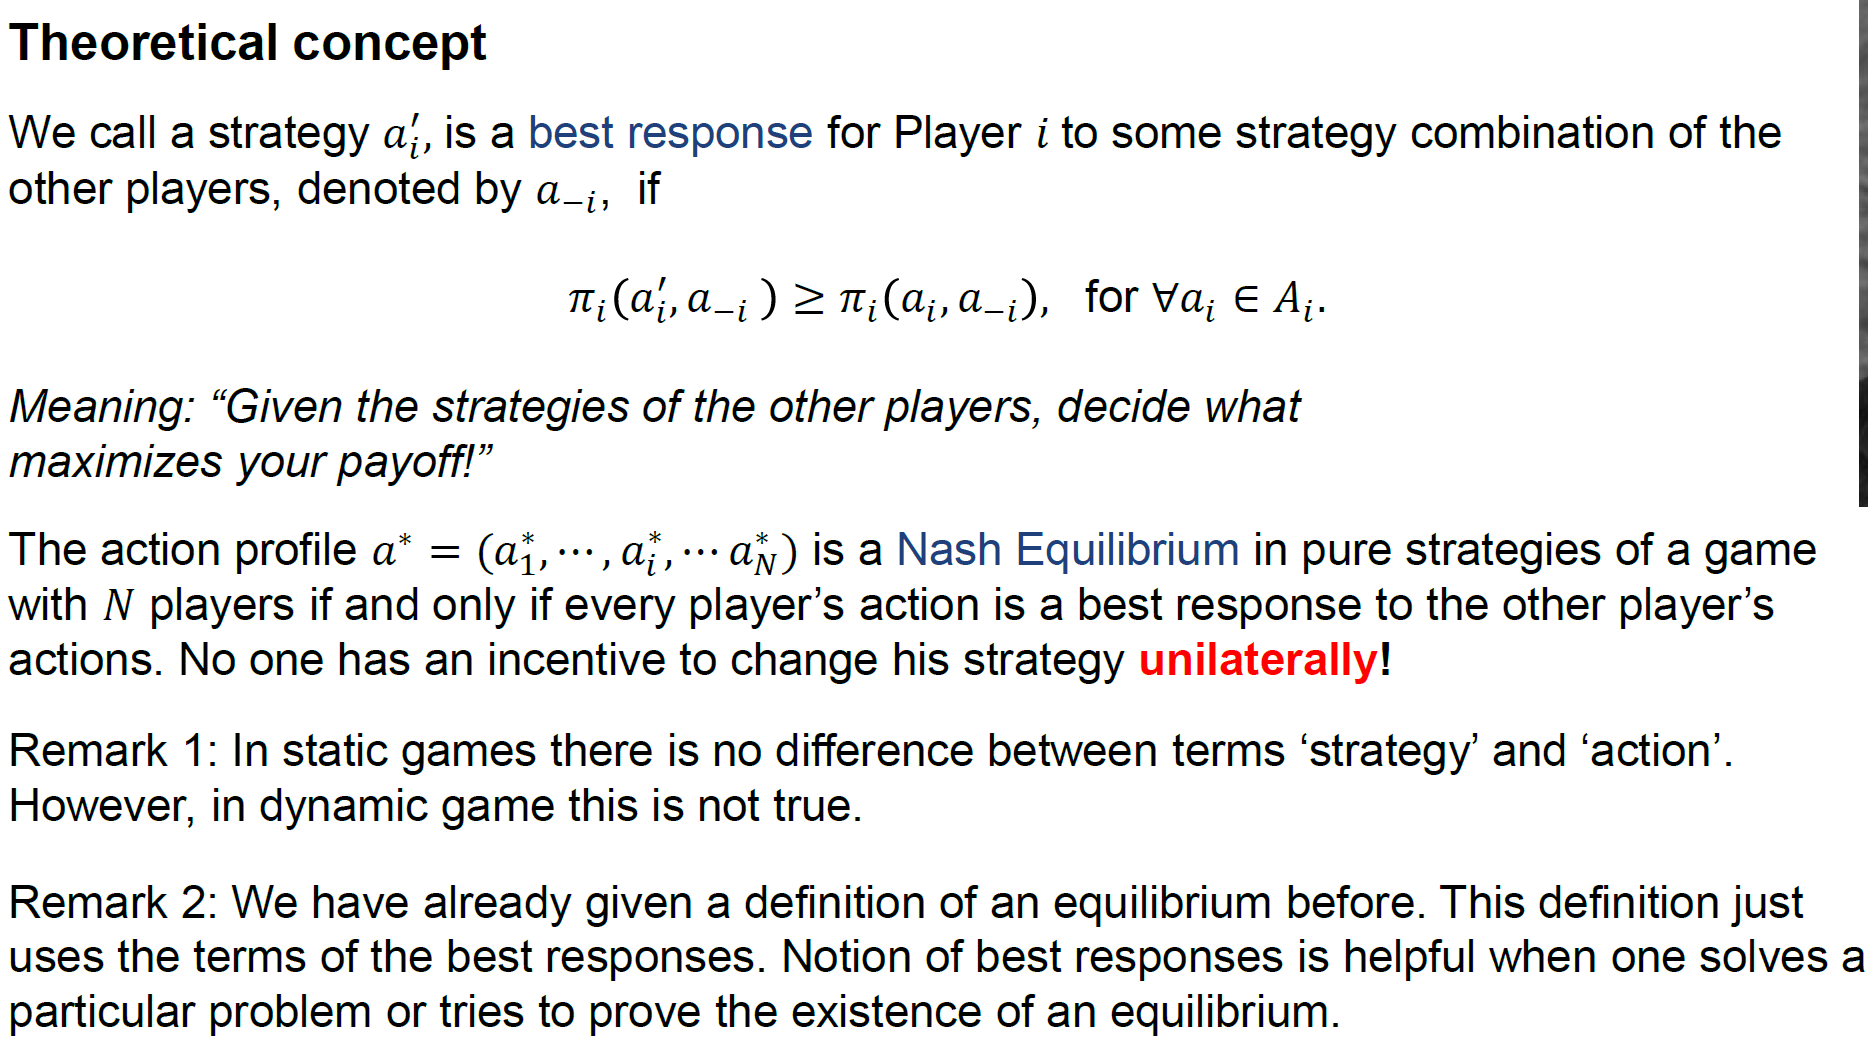
\includegraphics[width=0.6\textwidth]{Pictures/nash_equilibrium.png}
\end{figure}

Comments:
\begin{itemize}
    \item We applied two solution concepts $A$ and $B$: Maxmin by von Neumann
        and Nash Equilibrium.
    \item Both concepts let to the same solution.
    \item The maxmin cocept was developed first and is applicable to constant
        sum games.
    \item Nash's best response is more widely applicable and we will use it from
        now on.
\end{itemize}

Example 11: Equilibrium in pure strategies.

\begin{figure}[H]
    \centering
    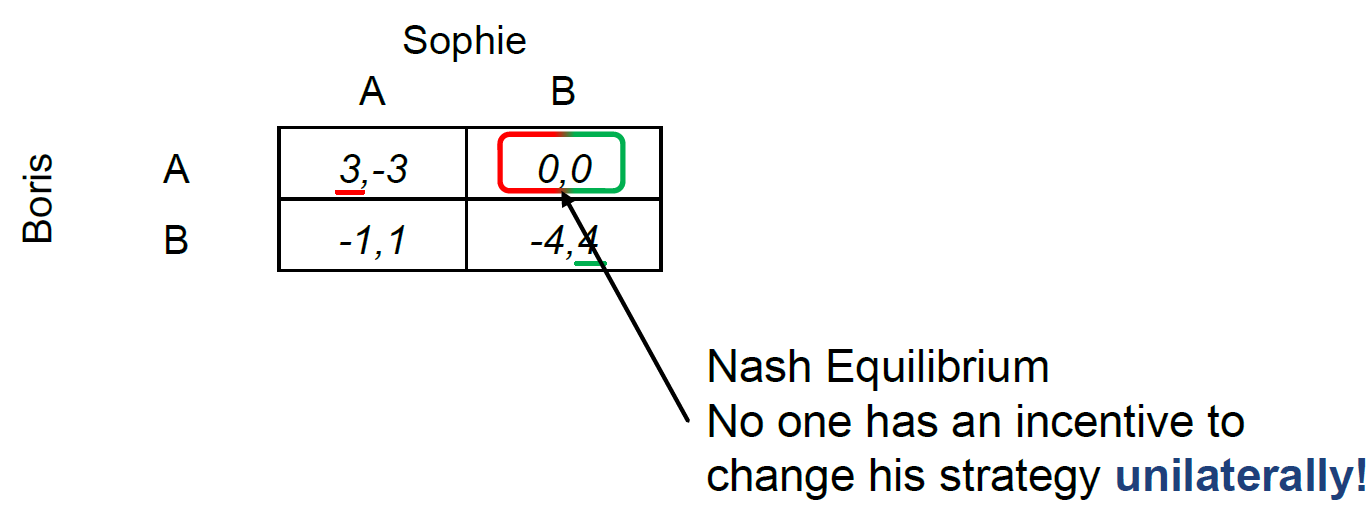
\includegraphics[width=0.5\textwidth]{Pictures/nash_equilibrium_2.png}
\end{figure}

Example 12: No equilibrium in pure strategies.

\begin{figure}[H]
    \centering
    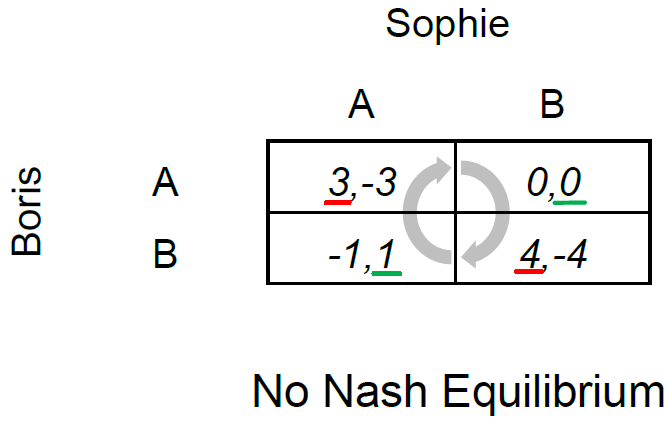
\includegraphics[width=0.4\textwidth]{Pictures/no_nash_equilibrium.png}
\end{figure}

\begin{figure}[H]
    \centering
    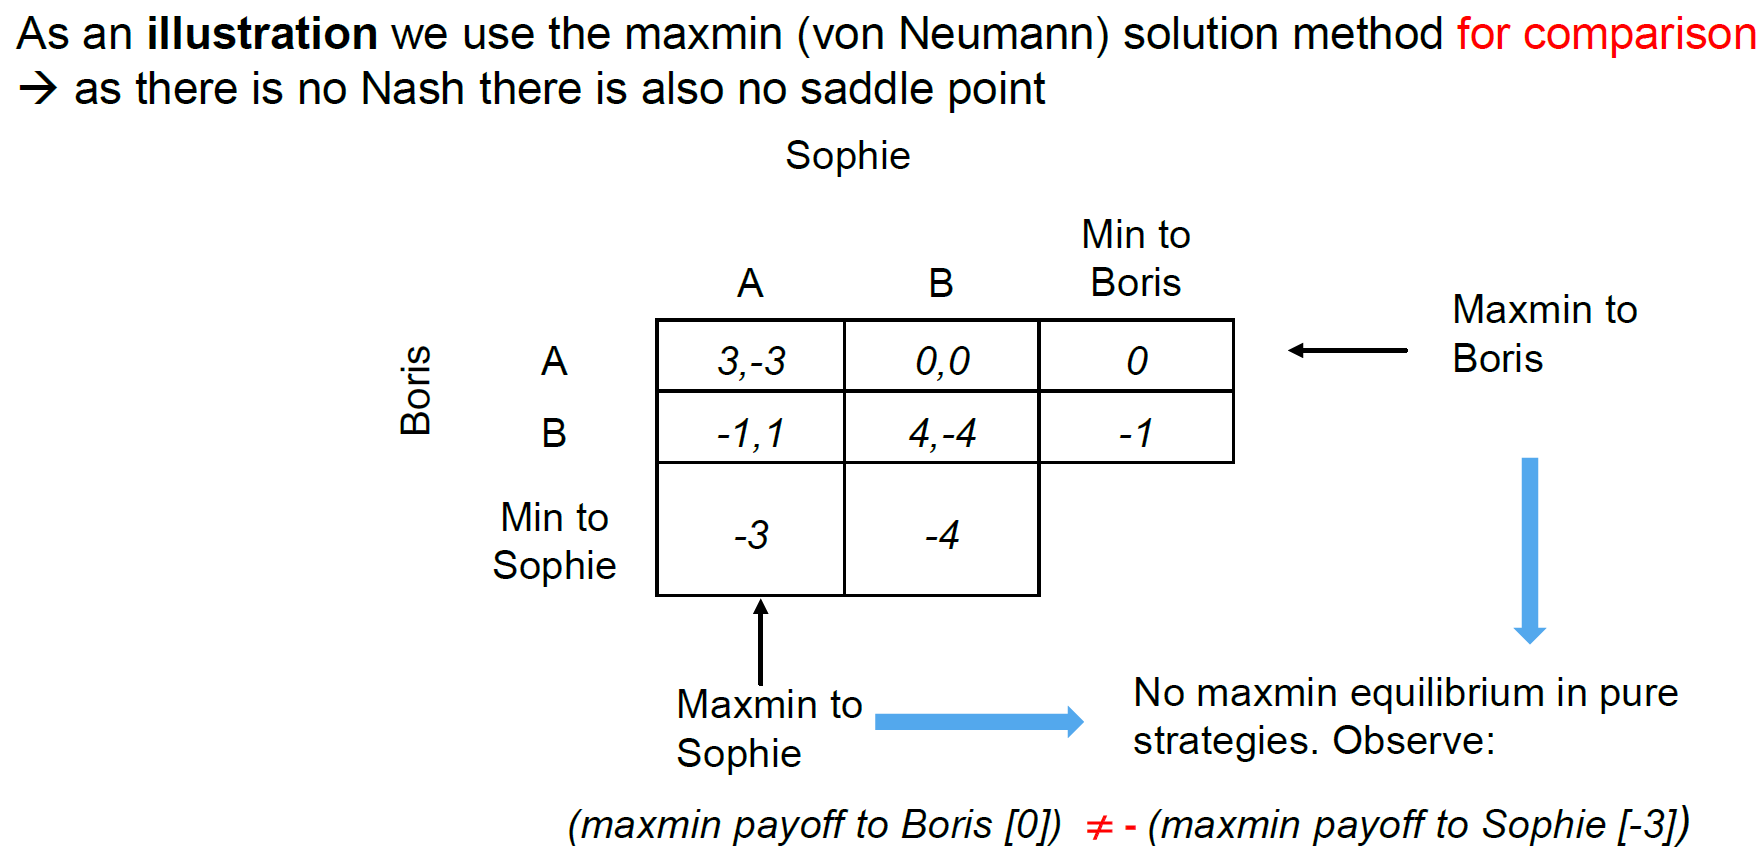
\includegraphics[width=0.6\textwidth]{Pictures/example_12_comment.png}
\end{figure}


Mixed Strategy:

\begin{itemize}
    \item A mixed Strategy specifies the probability with which each of the
        pure strategies is used.
    \item Example: Suppose the set of pure strategies to player $i$ is $S_i = \geschwungeneklammer{s_a,s_b,\dots}$
        Then the mixed strategy is a vector of probabilities
        $\sigma_i = \klammer{p(s_a) , p(s_b) , p(s_c) , \dots}$ such that
        $\sum_{s \in S_i} p(s) = 1$
    \item A pure strategy can pe represented as a special case of a mixed strategy.
\end{itemize}

Back to example 12:

\begin{figure}[H]
    \centering
    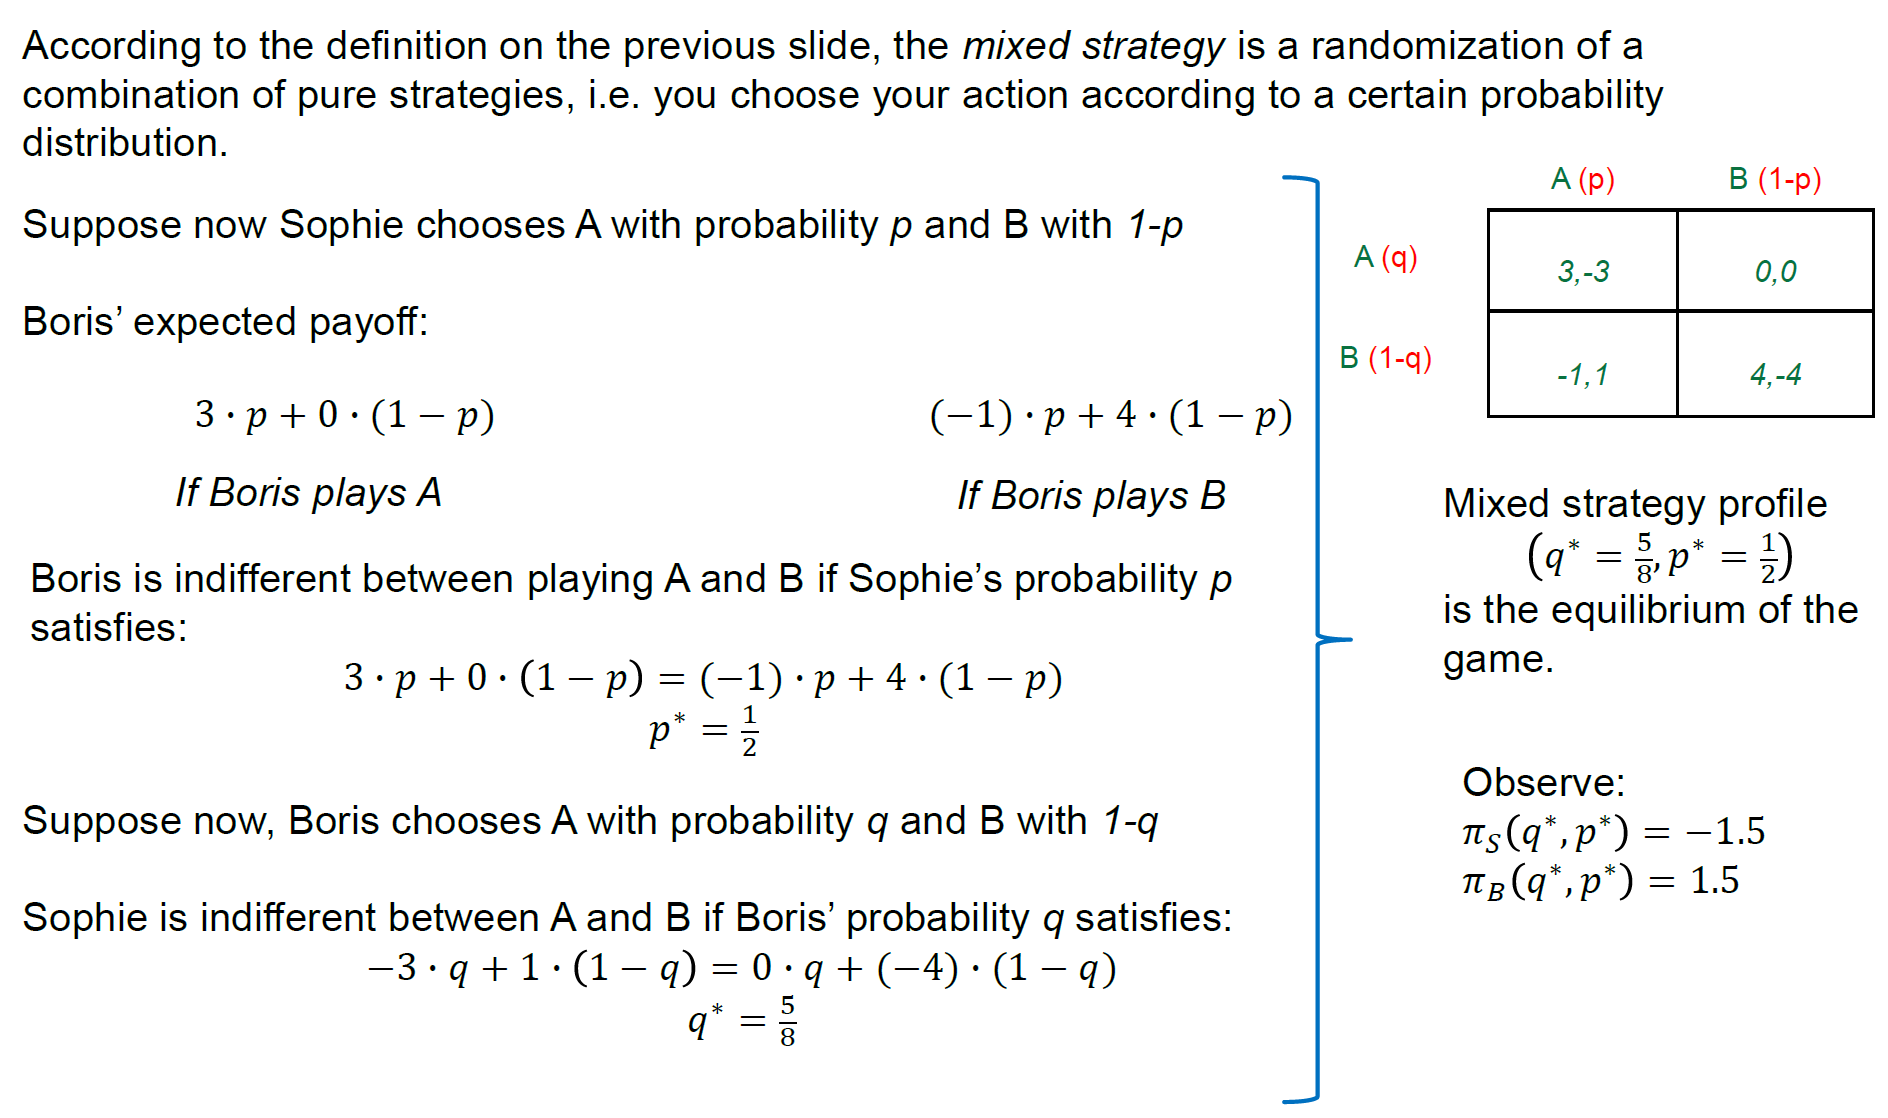
\includegraphics[width=0.7\textwidth]{Pictures/example_12_mixed_strategy.png}
\end{figure}

\subparagraph{Non constant sum game}

Example 13: Maroni game

\begin{figure}[H]
    \centering
    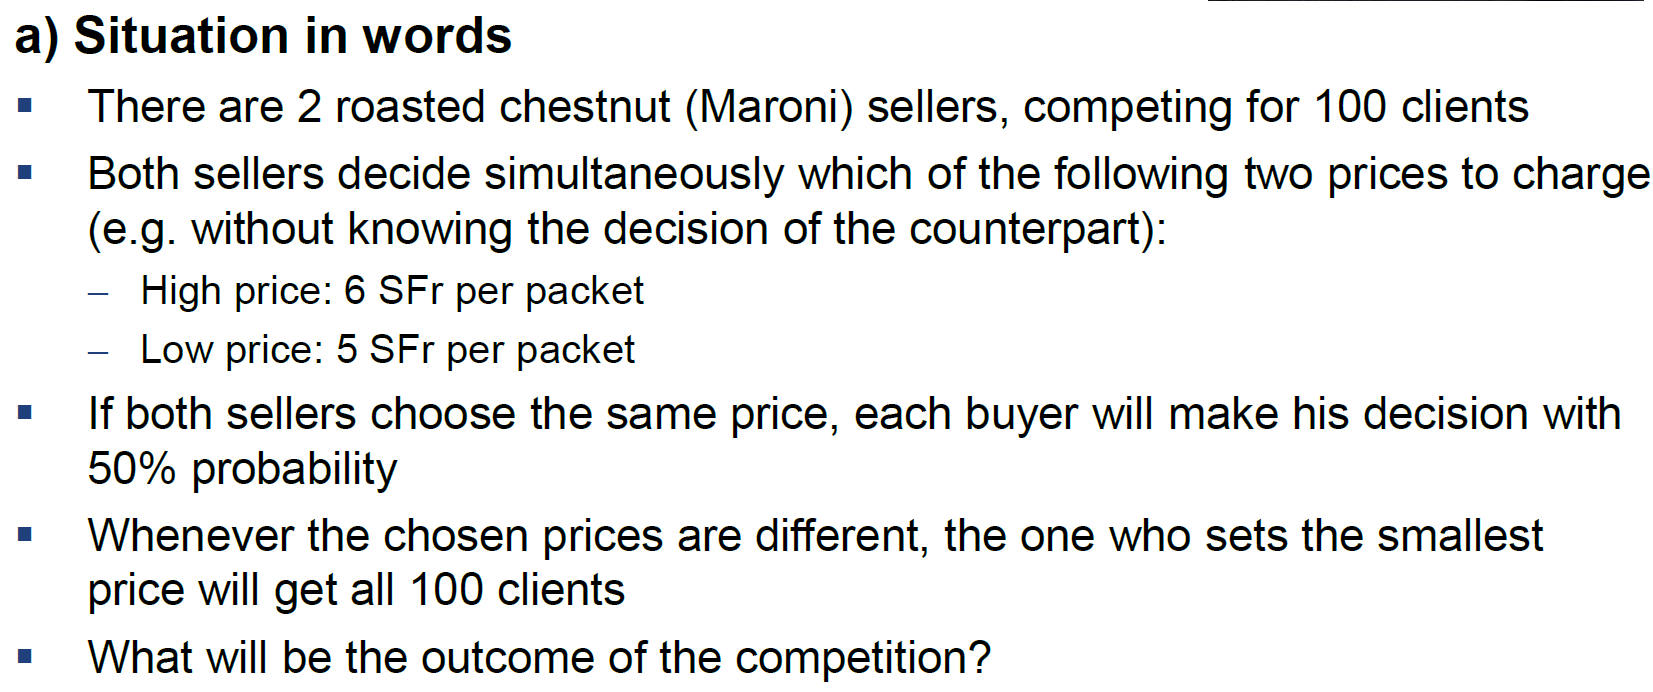
\includegraphics[width=0.6\textwidth]{Pictures/maroni1.png}
    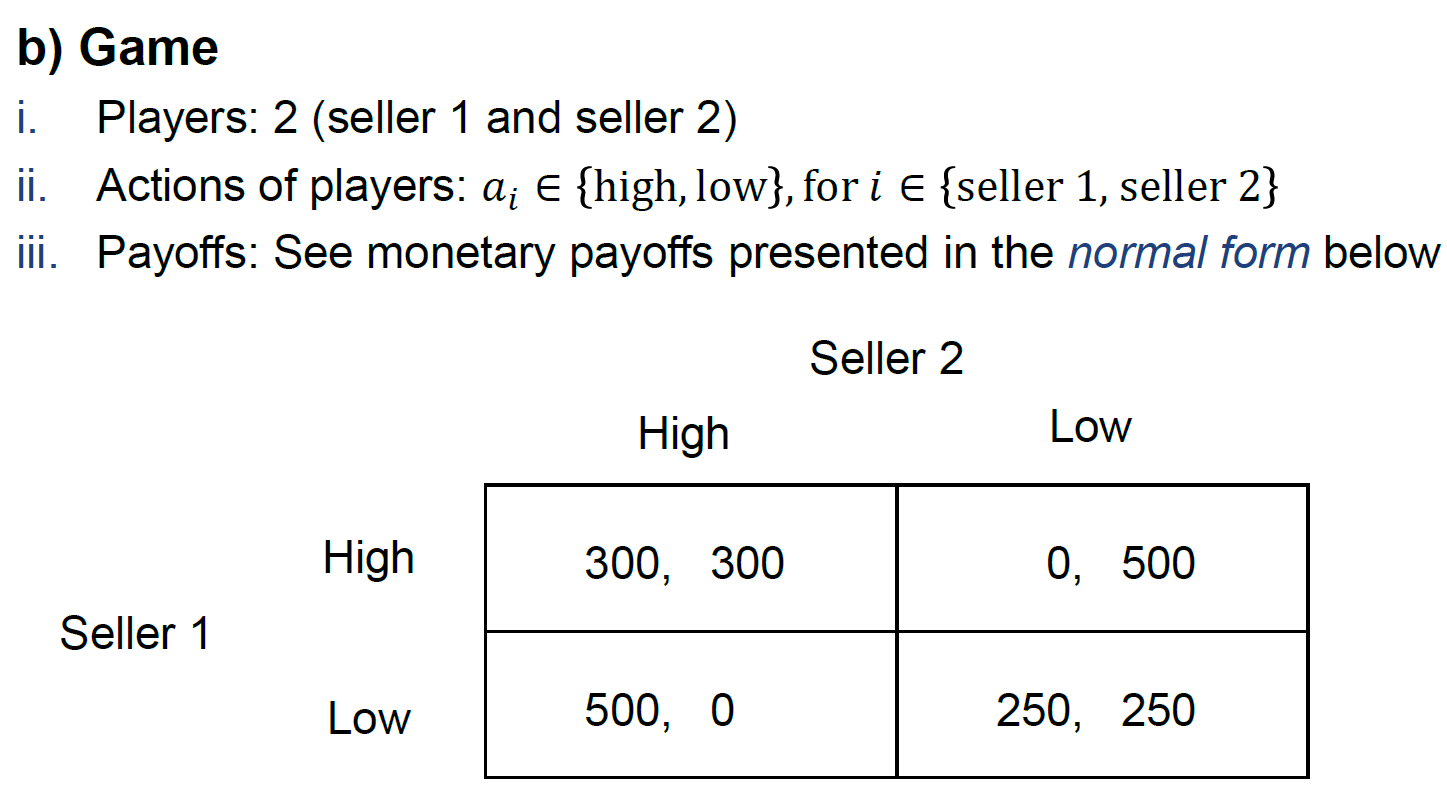
\includegraphics[width=0.6\textwidth]{Pictures/maroni2.png}
\end{figure}
Nash equilibrium at 250,250.

\begin{figure}[H]
    \centering
    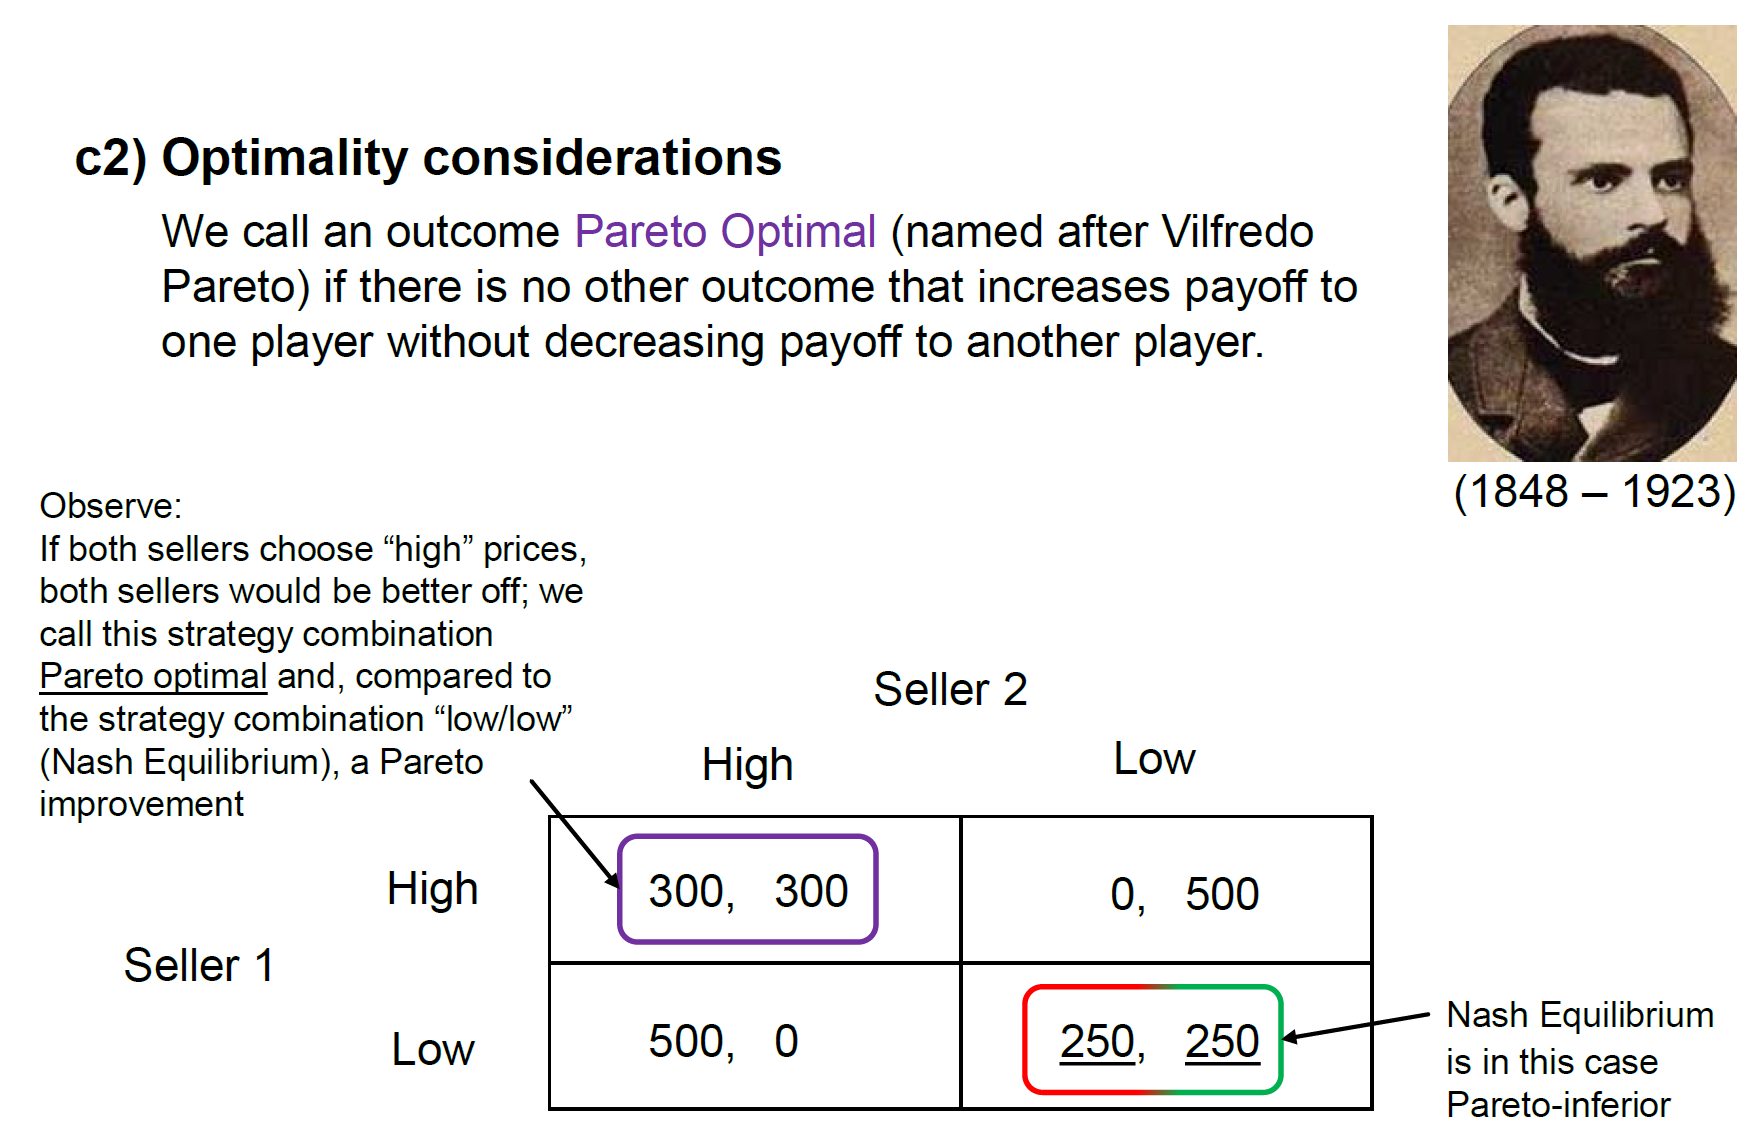
\includegraphics[width=0.5\textwidth]{Pictures/maroni3.png}
\end{figure}
"Low" is the dominant strategy.

\vspace{1\baselineskip}

Comments:
\begin{itemize}
    \item Game illustrates conflict in "economics"
    \item For both sellers strategy "low"-pricing dominates strategy "high"-pricing
    \item Nash Equilibrium is not always Pareto optimal outcome
    \item This is a typical illustration of the Prisoners' Dilemma
\end{itemize}

\vspace{1\baselineskip}

\underline{Classical Prisoners' Dilemma}

\begin{figure}[h]
    \centering
    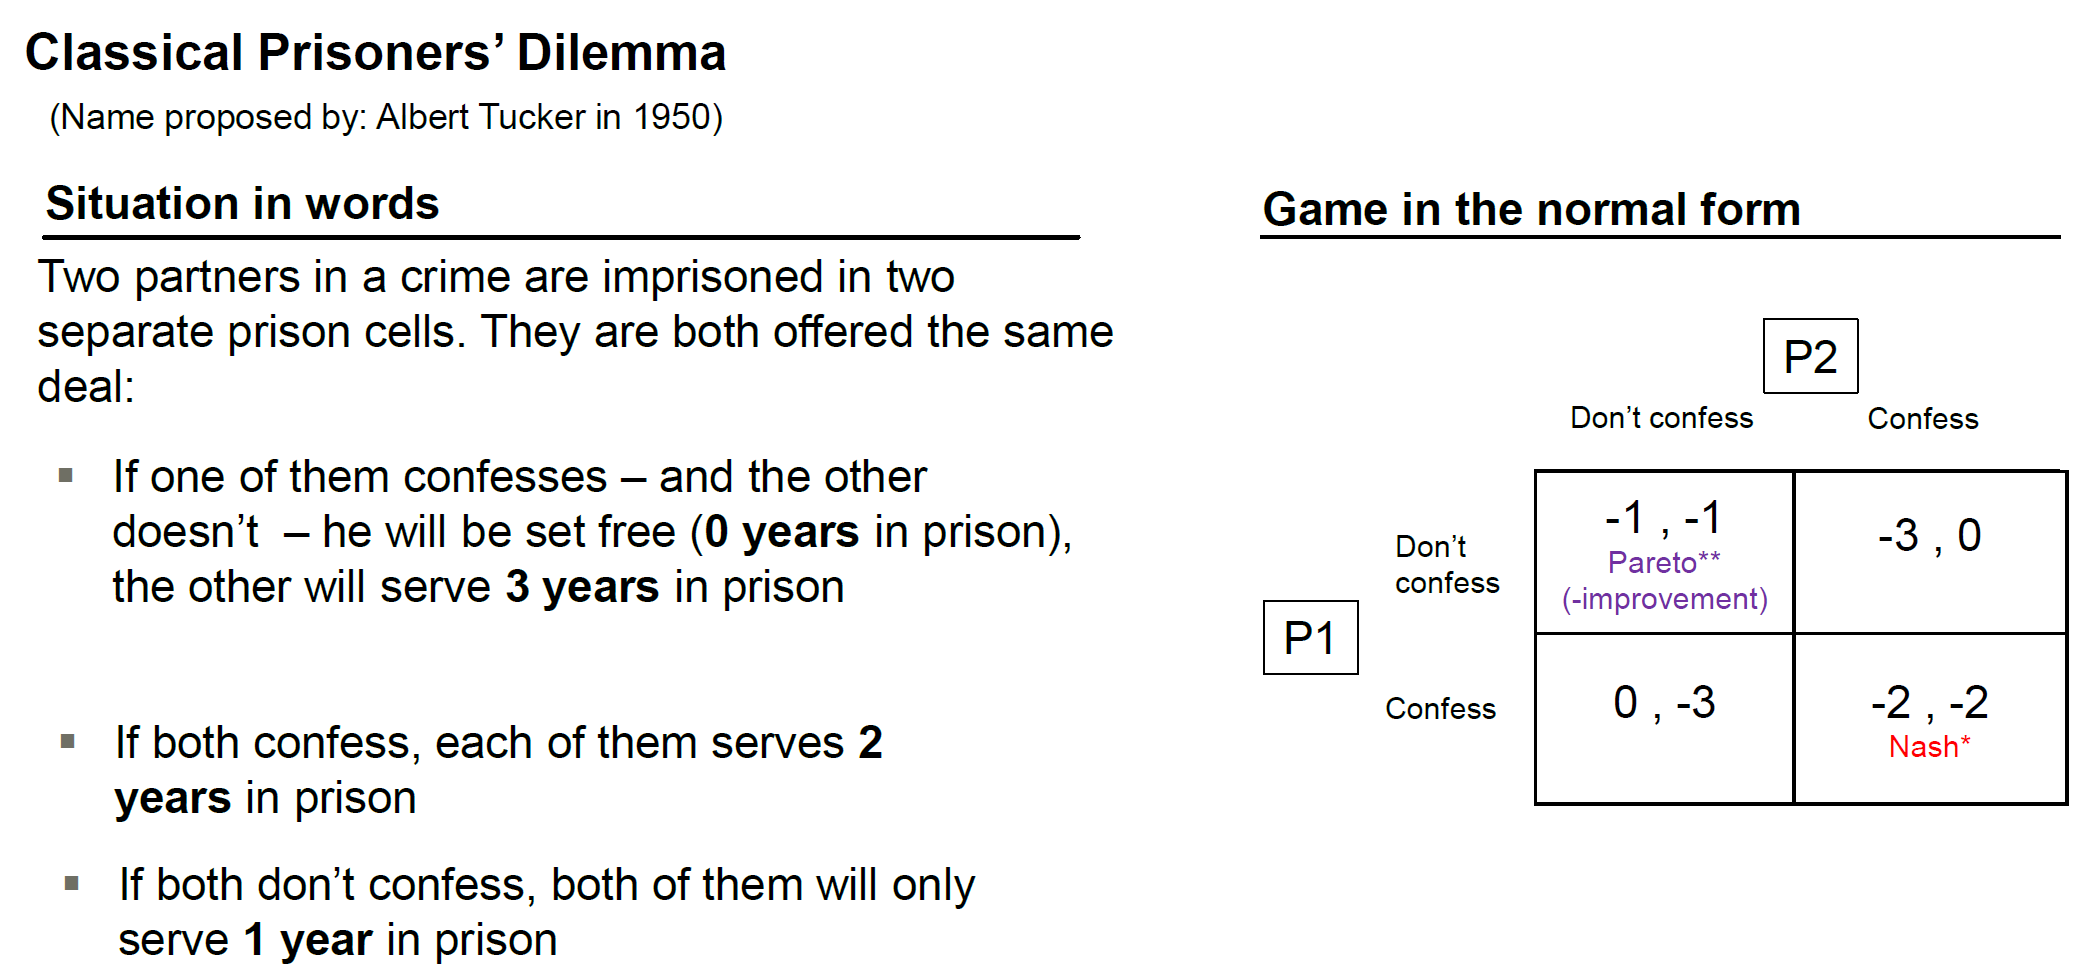
\includegraphics[width=0.7\textwidth]{Pictures/Prisoners_dilemma.png}
\end{figure}

\begin{figure}[H]
    \centering
    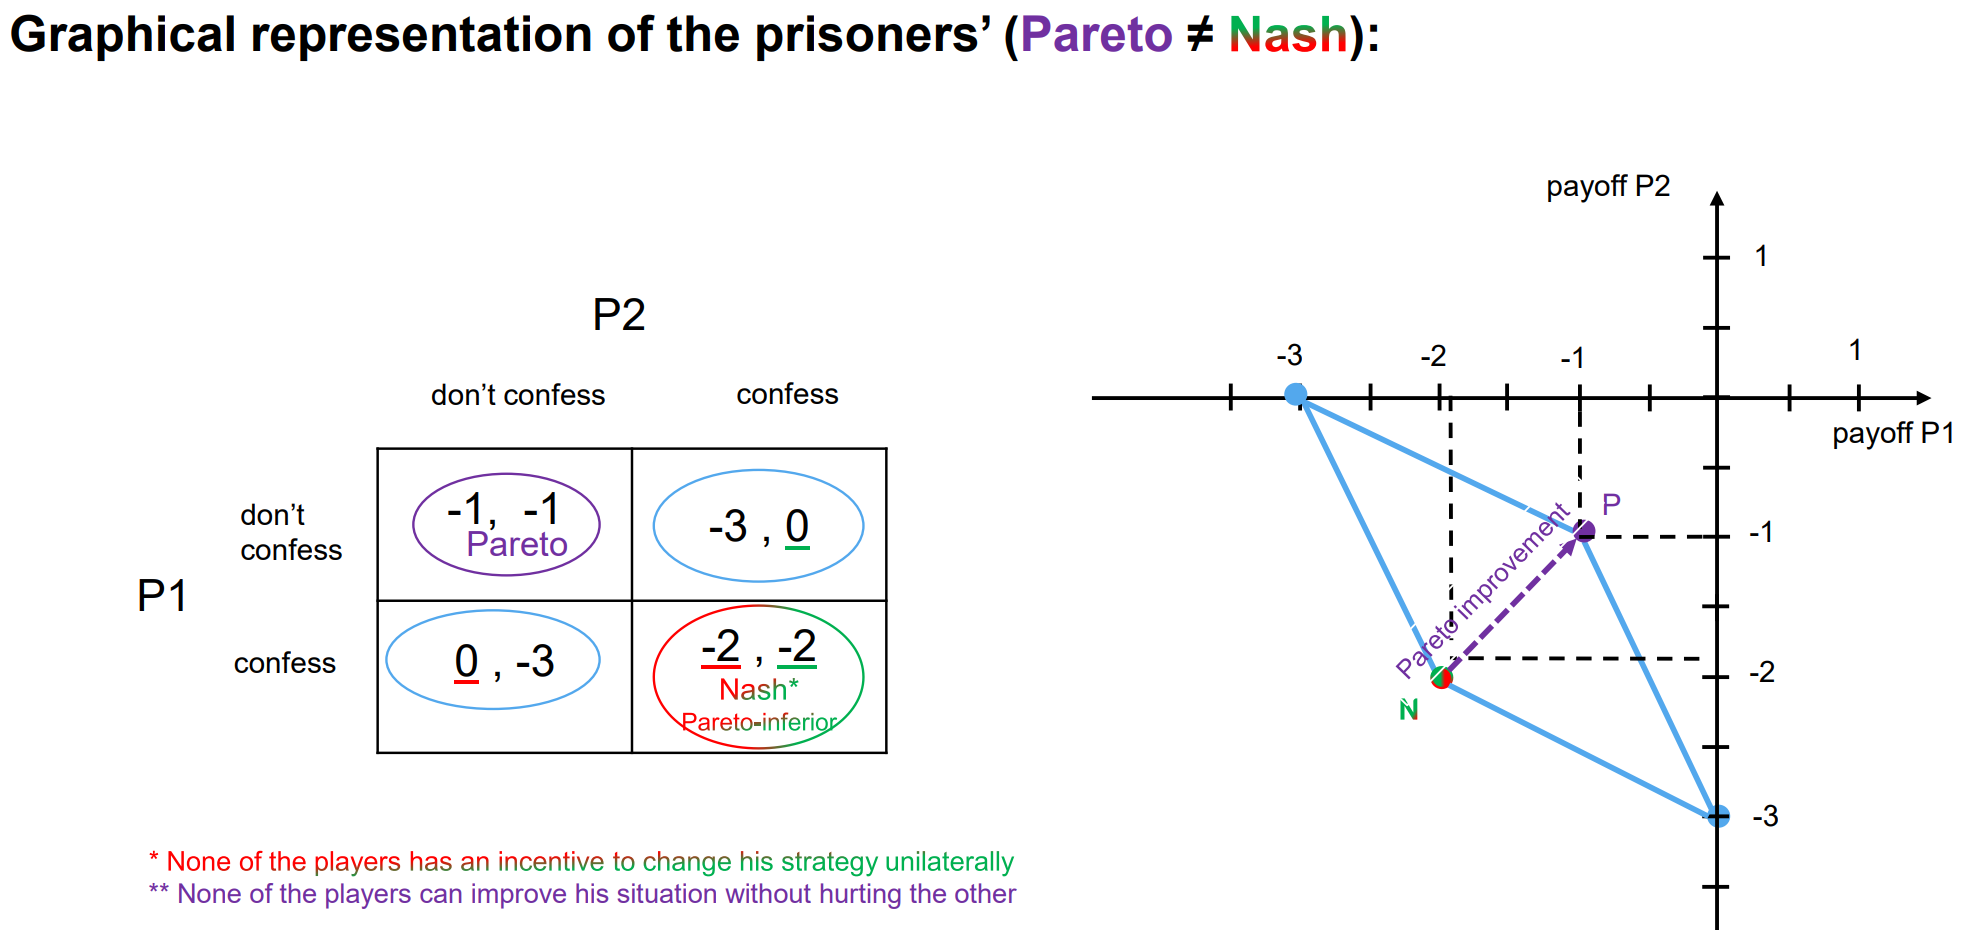
\includegraphics[width=0.8\textwidth]{Pictures/nash_pareto.png}
\end{figure}


\underline{Example 14:}
Situation:
\begin{itemize}
    \item Two countries disagree over the right of a patch of territory.
    \item The governments can decide whether to announce mobilization (and thus
        escalate conflict further) or to refrain from mobilization (and thus
        deescalate the conflict)
    \item When both countries decide to mobilize, the probability of war increases,
        while chances of peace resolution are getting smaller. This is the least
        preferred outcome for both countries as they fall in a devastating war
        (both receive utility of $0$)
    \item Whenever one country mobilizes and the other does not, the mobilizing
        army can get control over the territory without a war. This is the most
        attractive situation for the aggressor (utility of $4$) and the
        refraining country does not incur costs of war (utility of $2$).
    \item When both countries choose to refrain the likelihood of peaceful
        sharing of territory is high (utility of $3$).
\end{itemize}
Game:
\begin{enumerate}[(i)]
    \item Players: 2
    \item Actions of players: mobilize, refrain
    \item Payoffs: Summarized in normal form below:
\end{enumerate}

\begin{figure}[H]
    \centering
    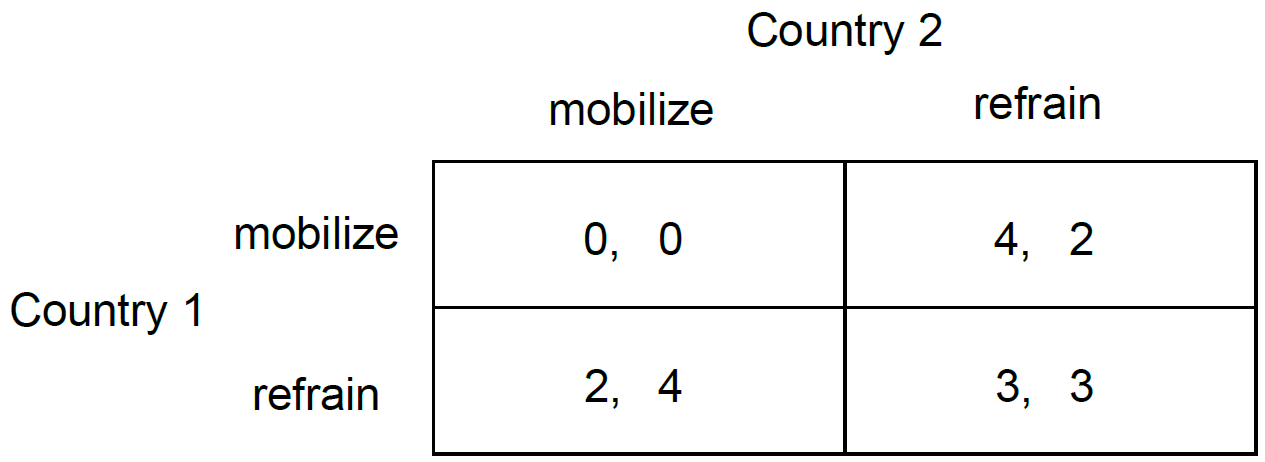
\includegraphics[width=0.5\textwidth]{Pictures/chicken_game.png}
\end{figure}

\begin{figure}[H]
    \centering
    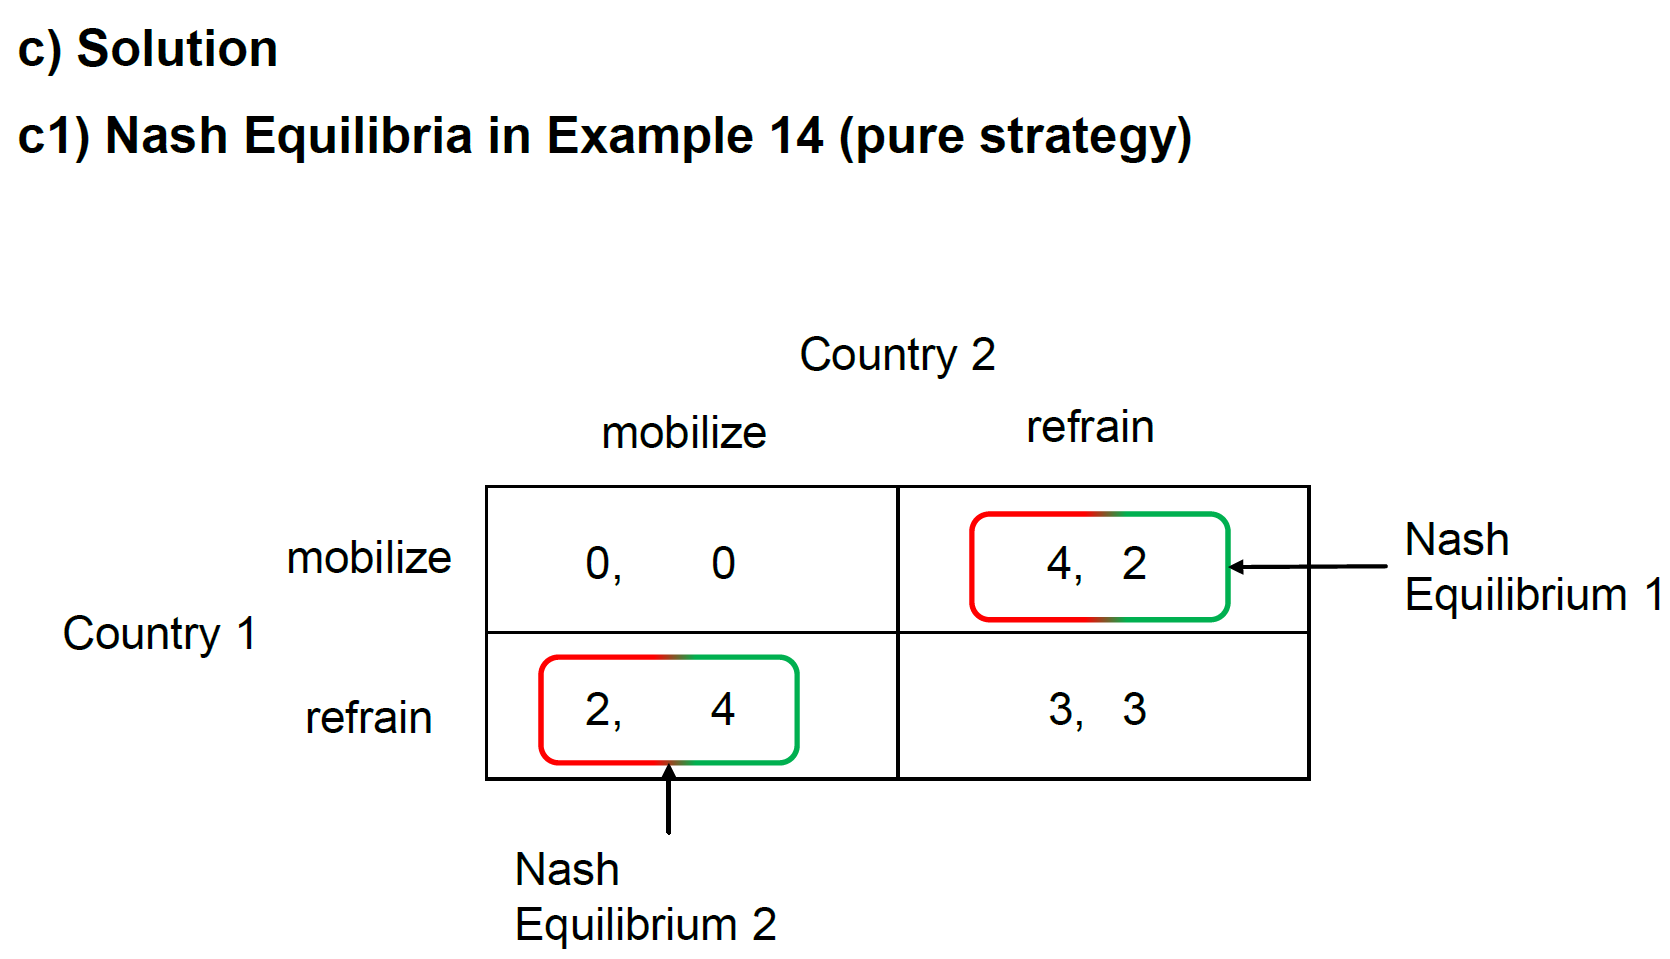
\includegraphics[width=0.5\textwidth]{Pictures/chicken_solution.png}
\end{figure}

\begin{figure}[H]
    \centering
    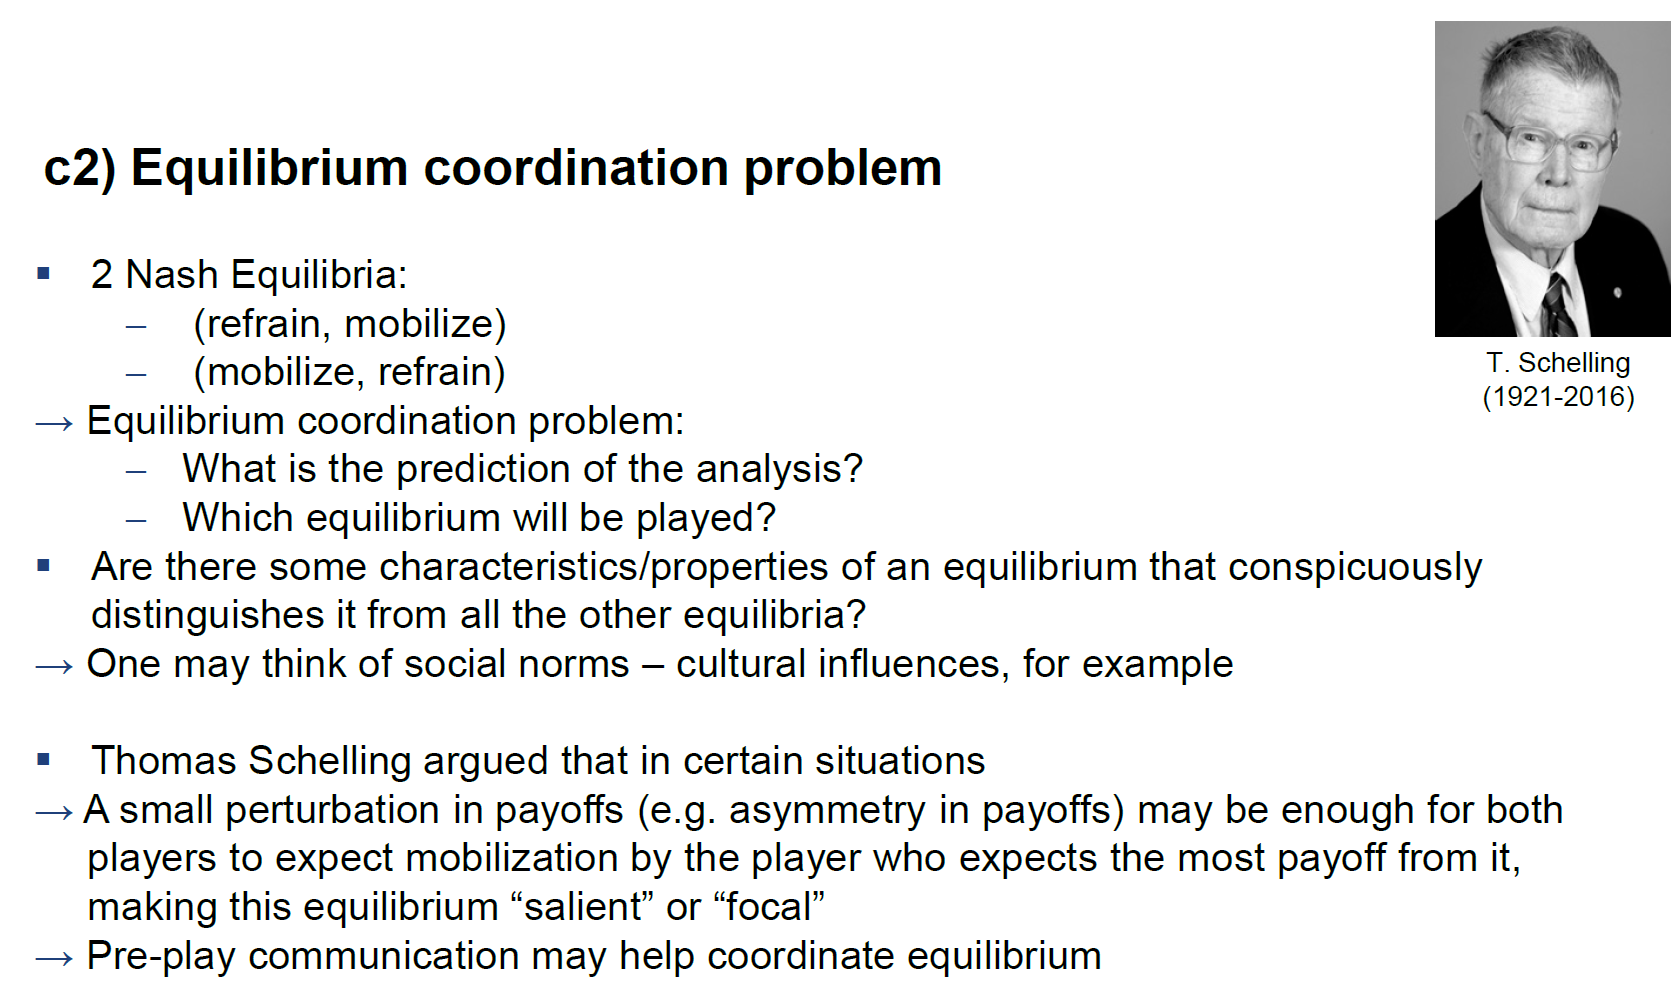
\includegraphics[width=0.7\textwidth]{Pictures/chicken_equilibrium.png}
\end{figure}

\begin{figure}[H]
    \centering
    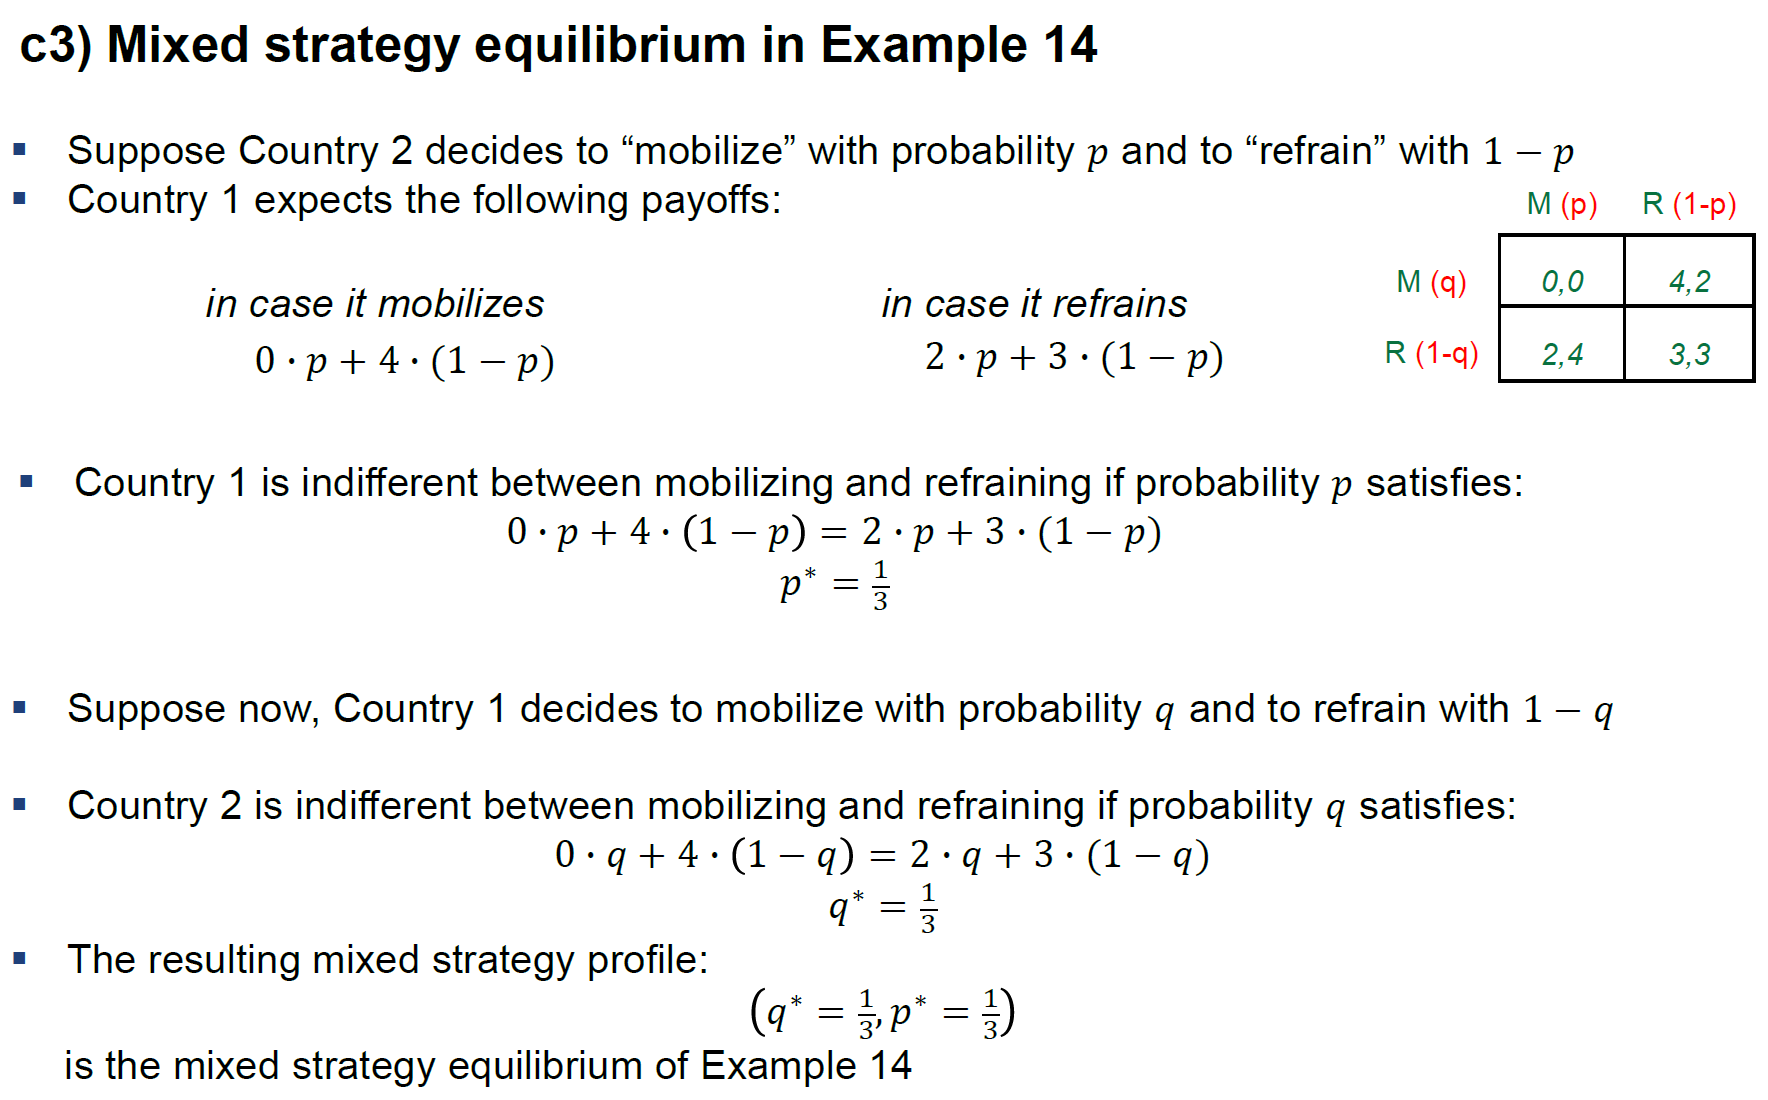
\includegraphics[width=0.6\textwidth]{Pictures/chicken_mixed_strategy.png}
\end{figure}

\begin{figure}[H]
    \centering
    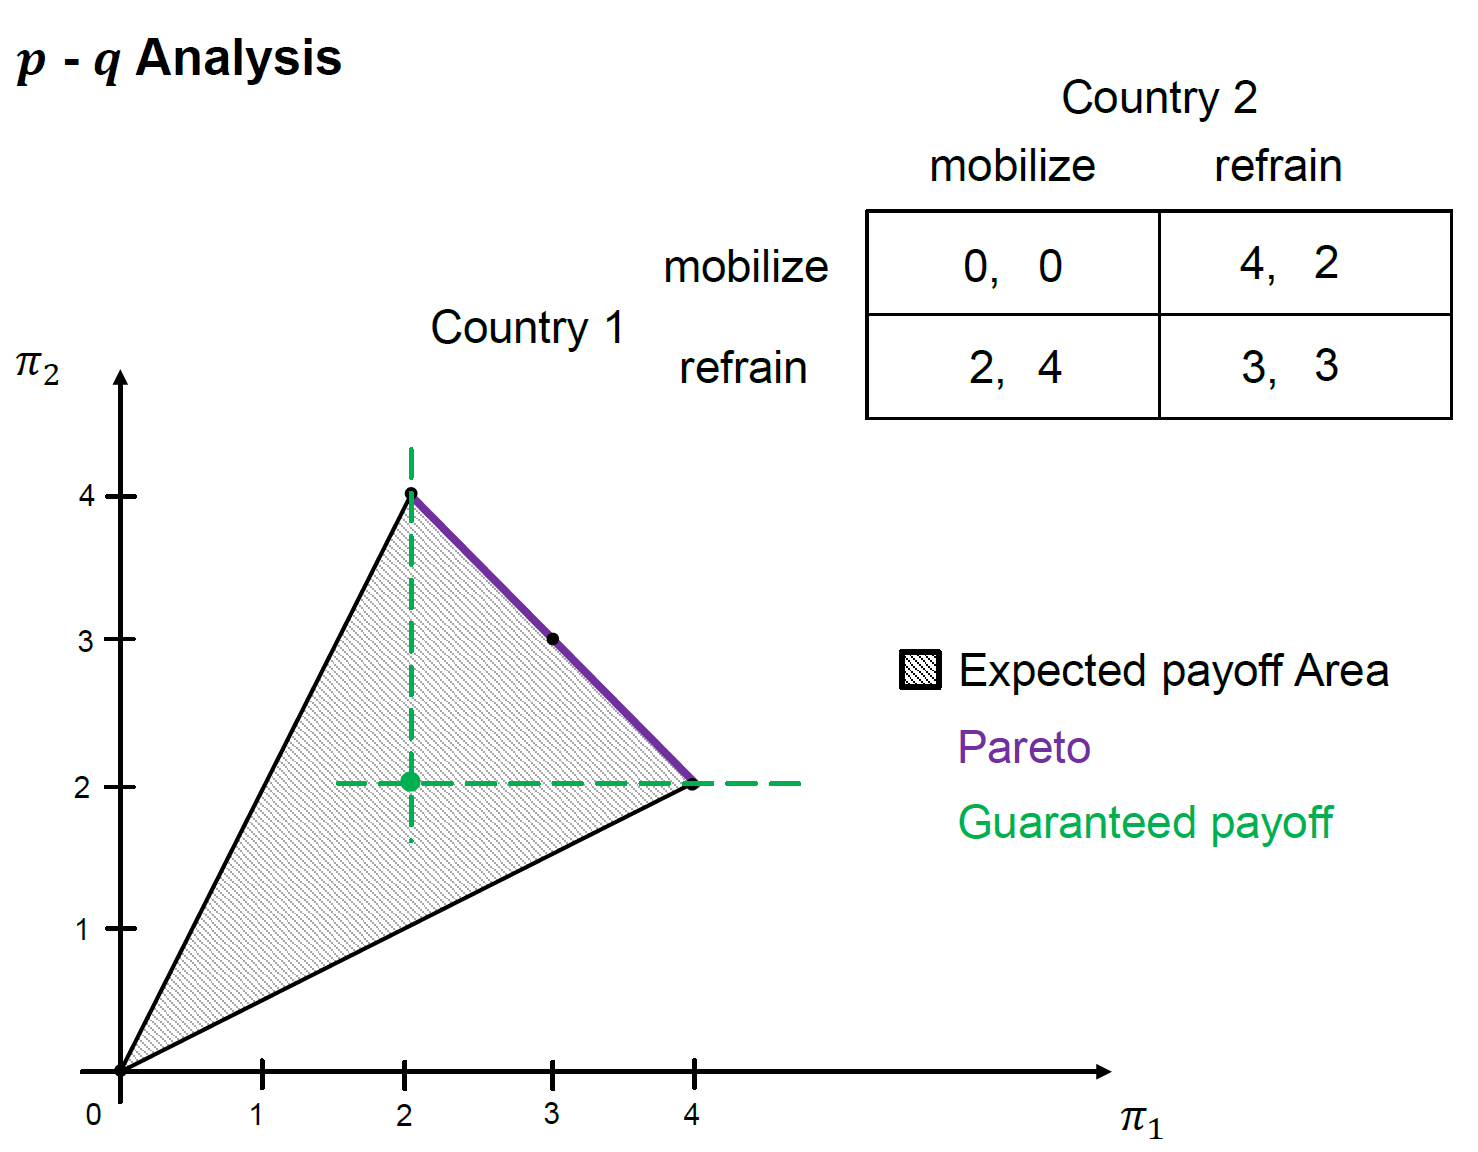
\includegraphics[width=0.5\textwidth]{Pictures/chicken_q_p_analysis.png}
\end{figure}

\begin{figure}[H]
    \centering
    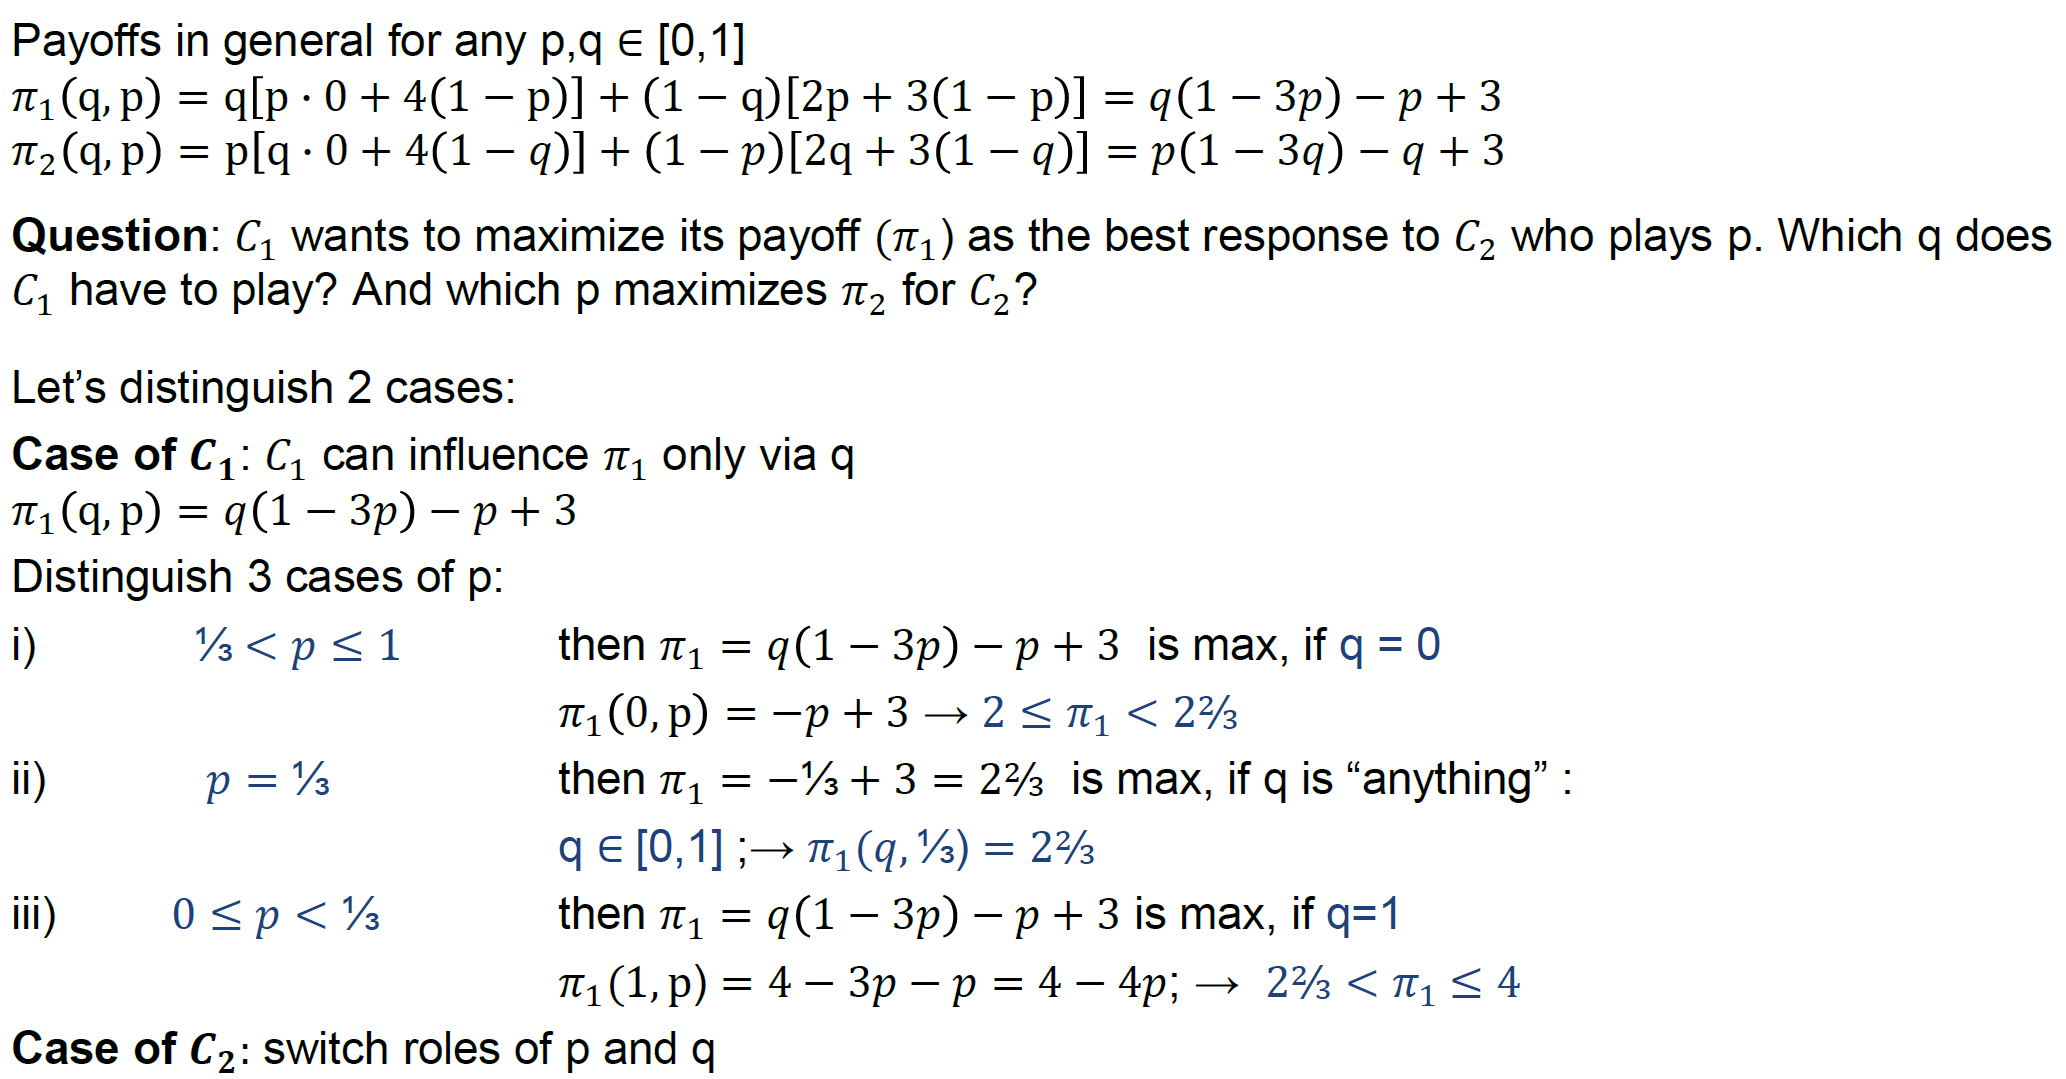
\includegraphics[width=0.7\textwidth]{Pictures/chicken_payoffs.png}
\end{figure}

\begin{figure}[H]
    \centering
    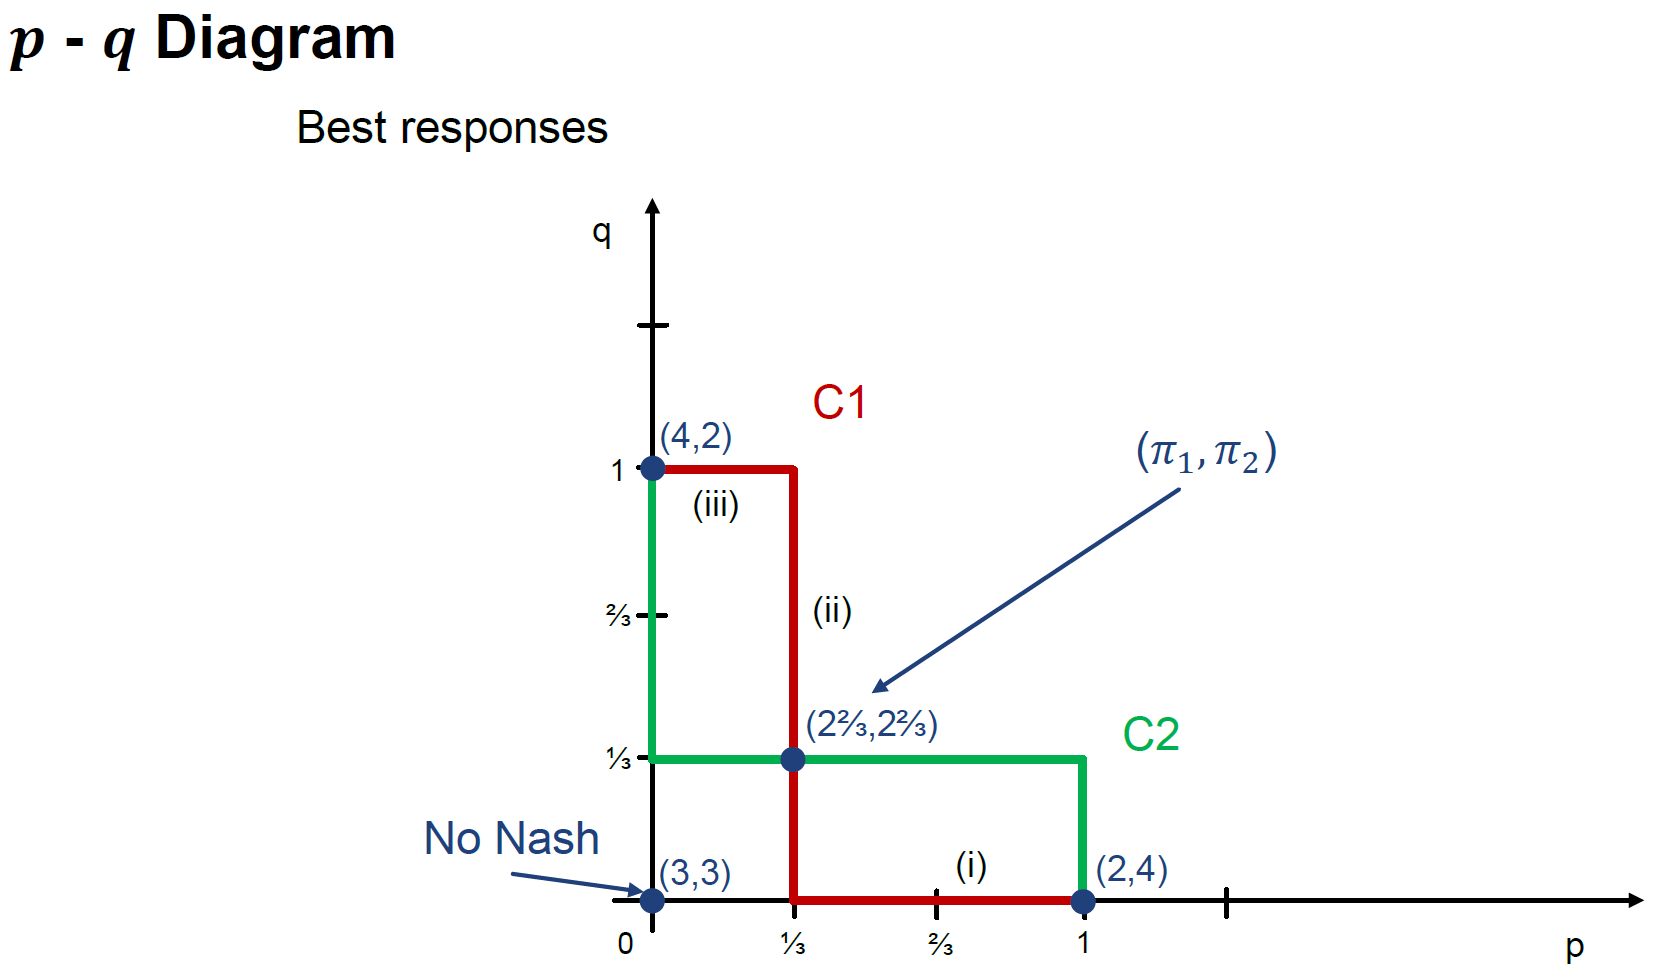
\includegraphics[width=0.5\textwidth]{Pictures/chicken_p_g_diagram.png}
\end{figure}

Comments:
\begin{itemize}
    \item This type of game is often referred to "Chicken" or "Hawk-Dove" game.
        The name is derived from a "sport" in which two drivers race towards each other
        on a narrow road. Each driver has the option to either swerve or to
        continue on a collision course.
    \item In case of multiple equilibria - how to coordinate a particular outcome?
    \item There can be one, many or no Nash equilibria in pure strategy
    \item Existance of Nash Equilibrium: In the normal-form game with a finite
        number of players and each player's strategy set being finite, there
        exists at least one Nash Equilibrium in pure or mixed strategies.
\end{itemize}

\begin{figure}[H]
    \centering
    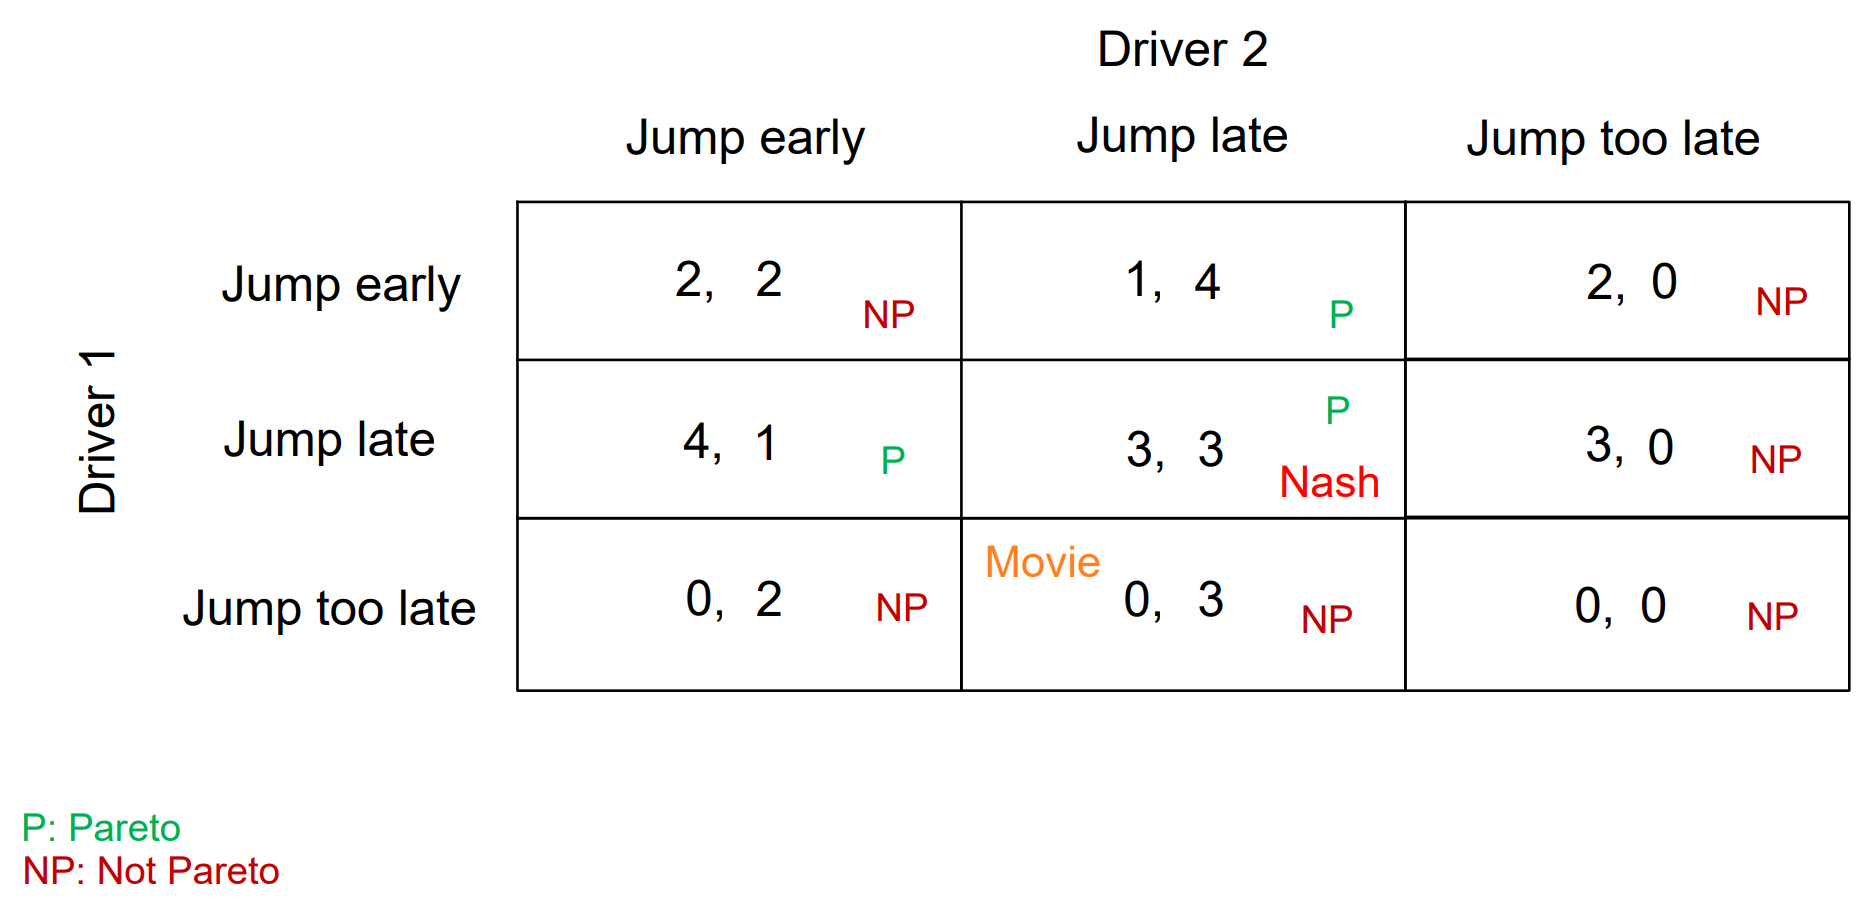
\includegraphics[width=0.6\textwidth]{Pictures/chicken_driver_solution.png}
\end{figure}

\vspace{1\baselineskip}

\underline{Example 15: Stag Hunt}
Situation:
\begin{itemize}
    \item The "Stag Hunt" is a game extracted from Jean Jaques Rousseau's
        "A Discourse on Inequality" which introduces the conflict between
        cooperation and safety.
    \item In this game, each member of a group of hunters has two options:
        he may remain attentive to the pursuit of the stag, or he may catch a hare
    \item If all hunters cooperate to pursue the stag, they catch it and share it
        equally; if any hunter devotes his energy to catching a hare, the stag
        escapes, and the hare belongs to de defecting hunter hunter alone
    \item Each hunter prefers a share of the stag to the hare
\end{itemize}


\begin{figure}[H]
    \centering
    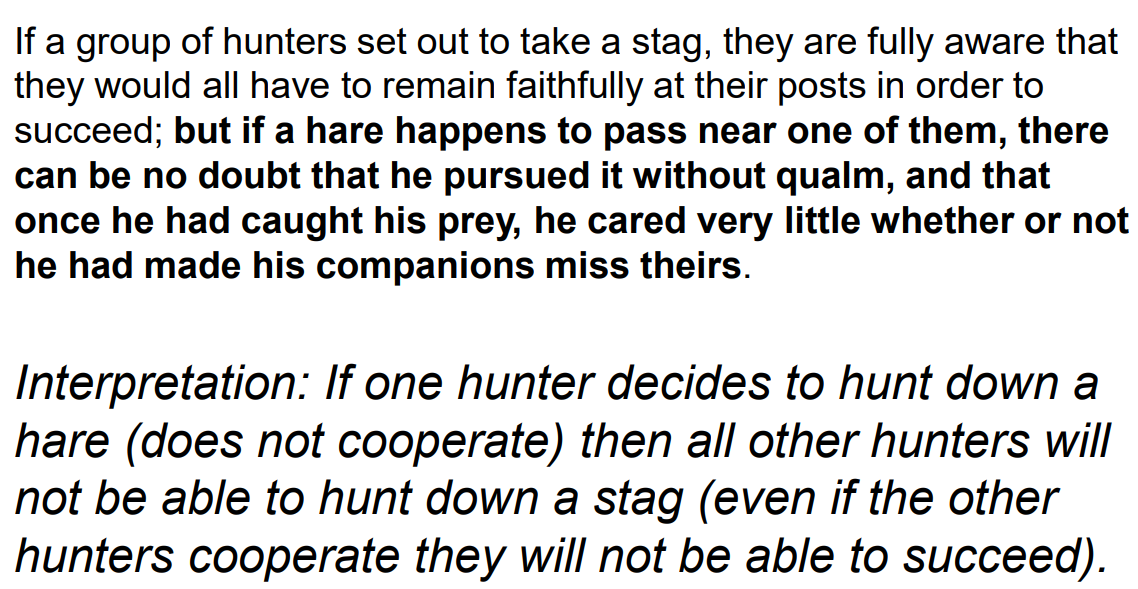
\includegraphics[width=0.5\textwidth]{Pictures/rousseau.png}
\end{figure}

Game:
\begin{enumerate}[(i)]
    \item Players: 2
    \item Actions of players: Stag, Hare
    \item Payoffs are presented in the normal form below
\end{enumerate}

\begin{figure}[H]
    \centering
    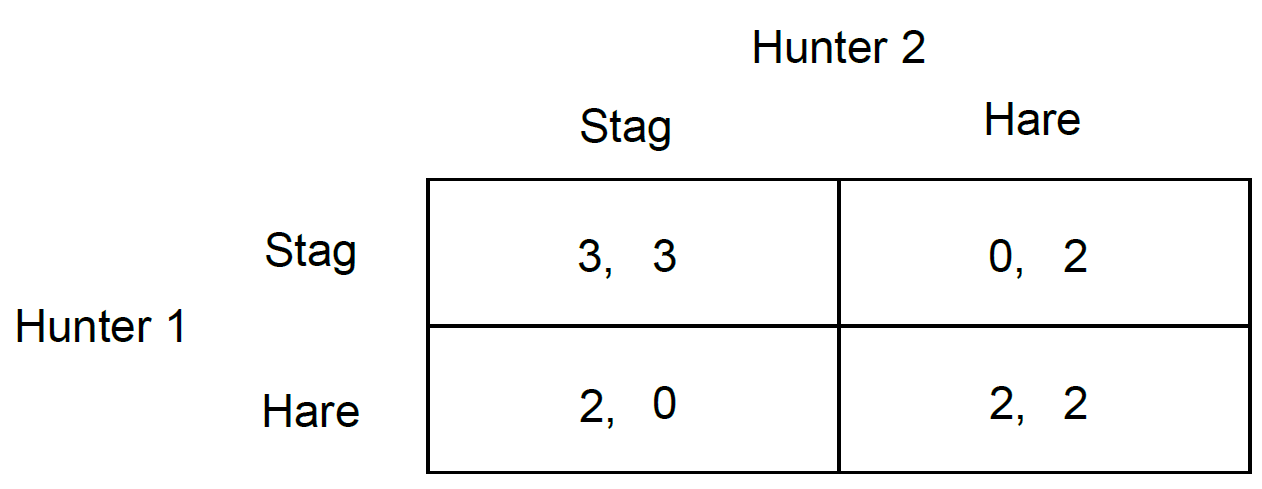
\includegraphics[width=0.5\textwidth]{Pictures/stag_hare_hunter.png}
\end{figure}

\begin{figure}[H]
    \centering
    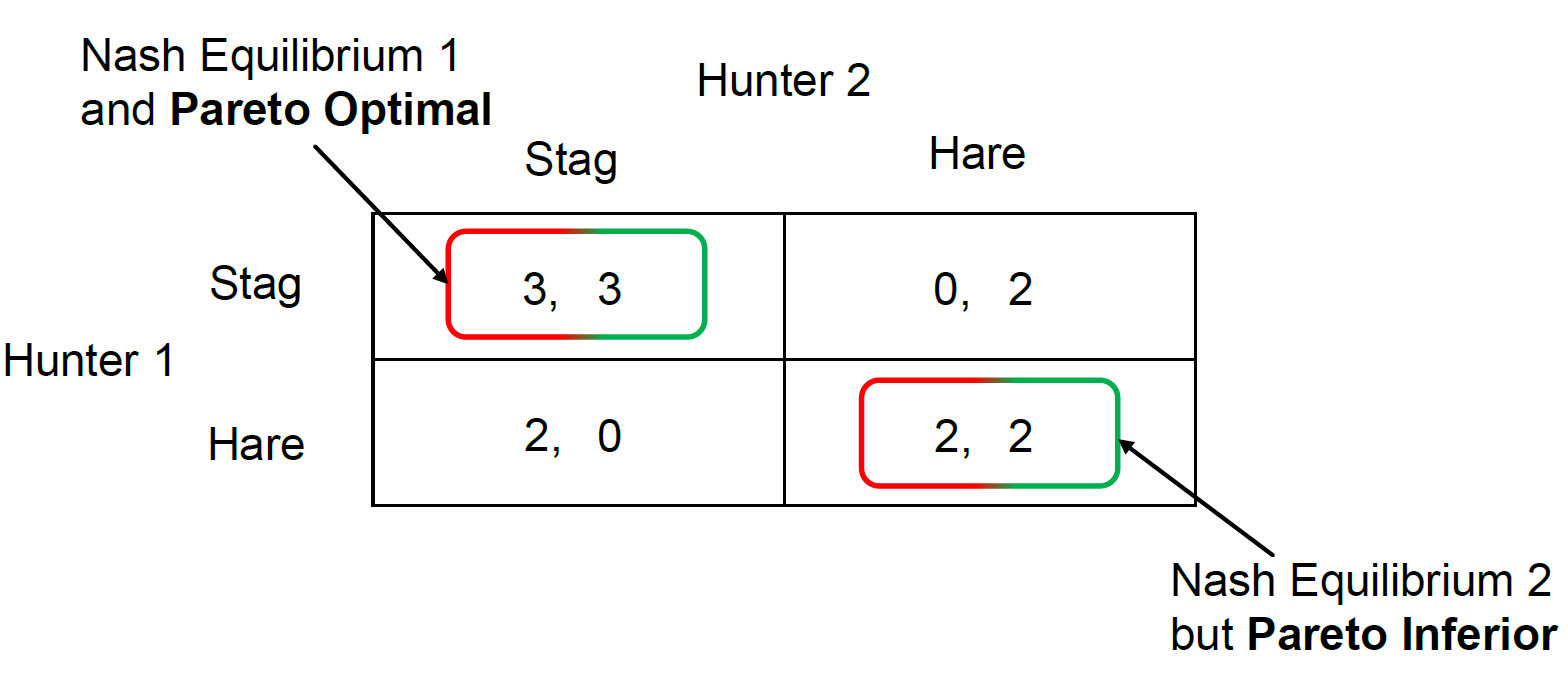
\includegraphics[width=0.5\textwidth]{Pictures/hunter_pure_strategy.png}
    \caption{Pure Strategy}
\end{figure}

\begin{figure}[H]
    \centering
    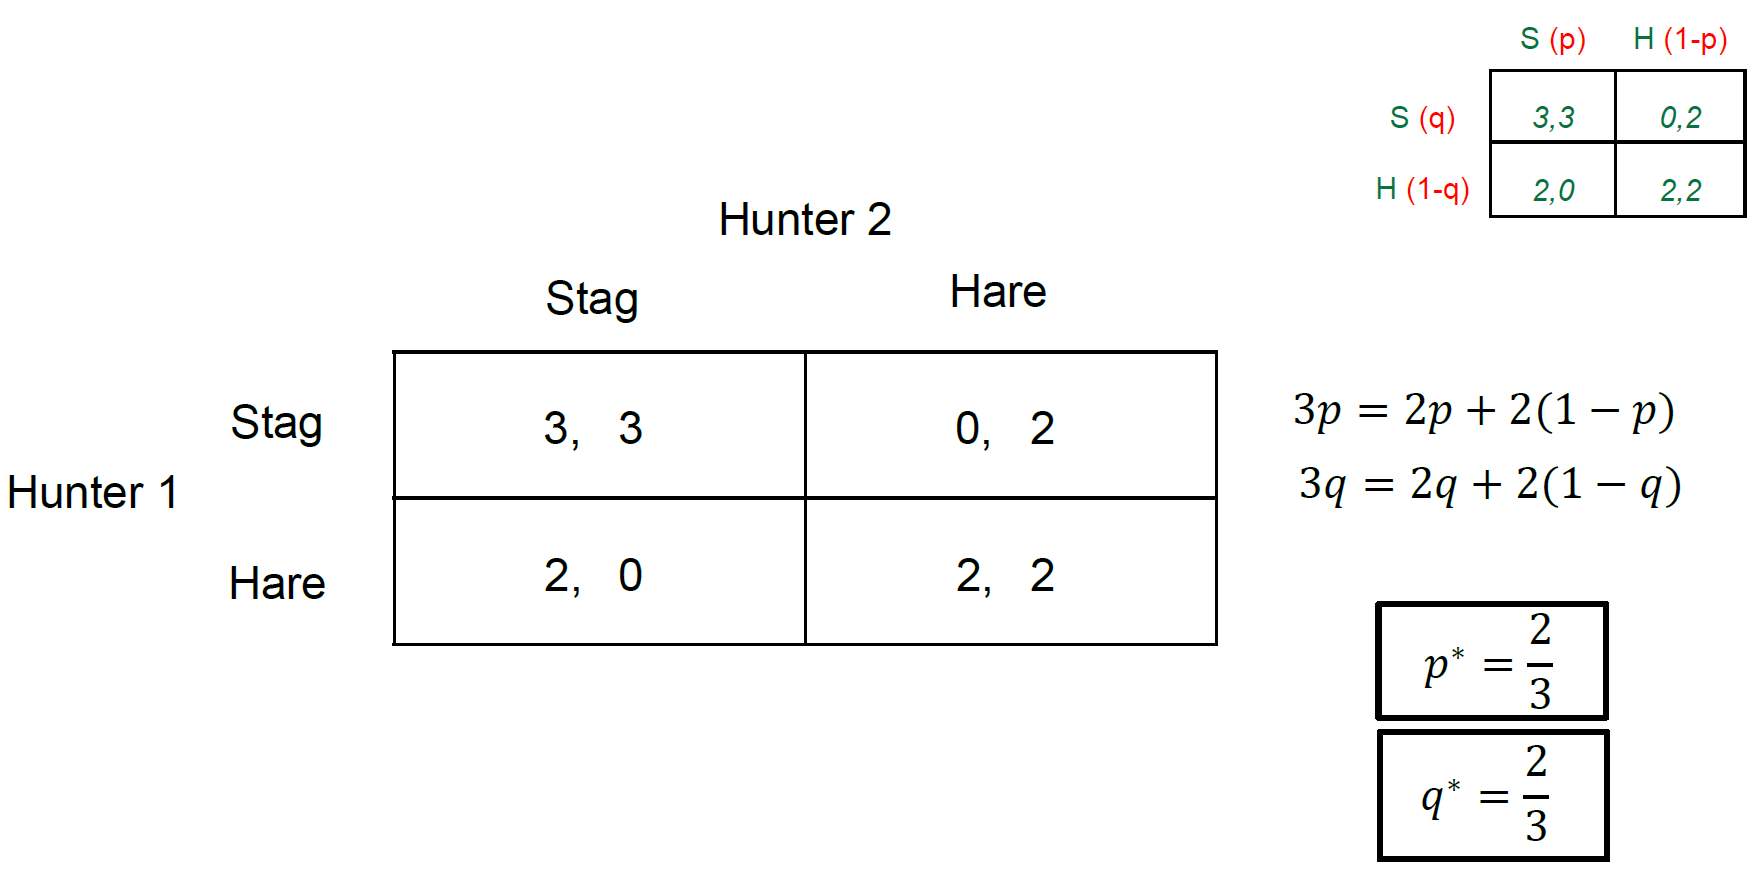
\includegraphics[width=0.5\textwidth]{Pictures/hunter_mixed_strategy.png}
    \caption{Mixed Strategy}
\end{figure}

\begin{figure}[H]
    \centering
    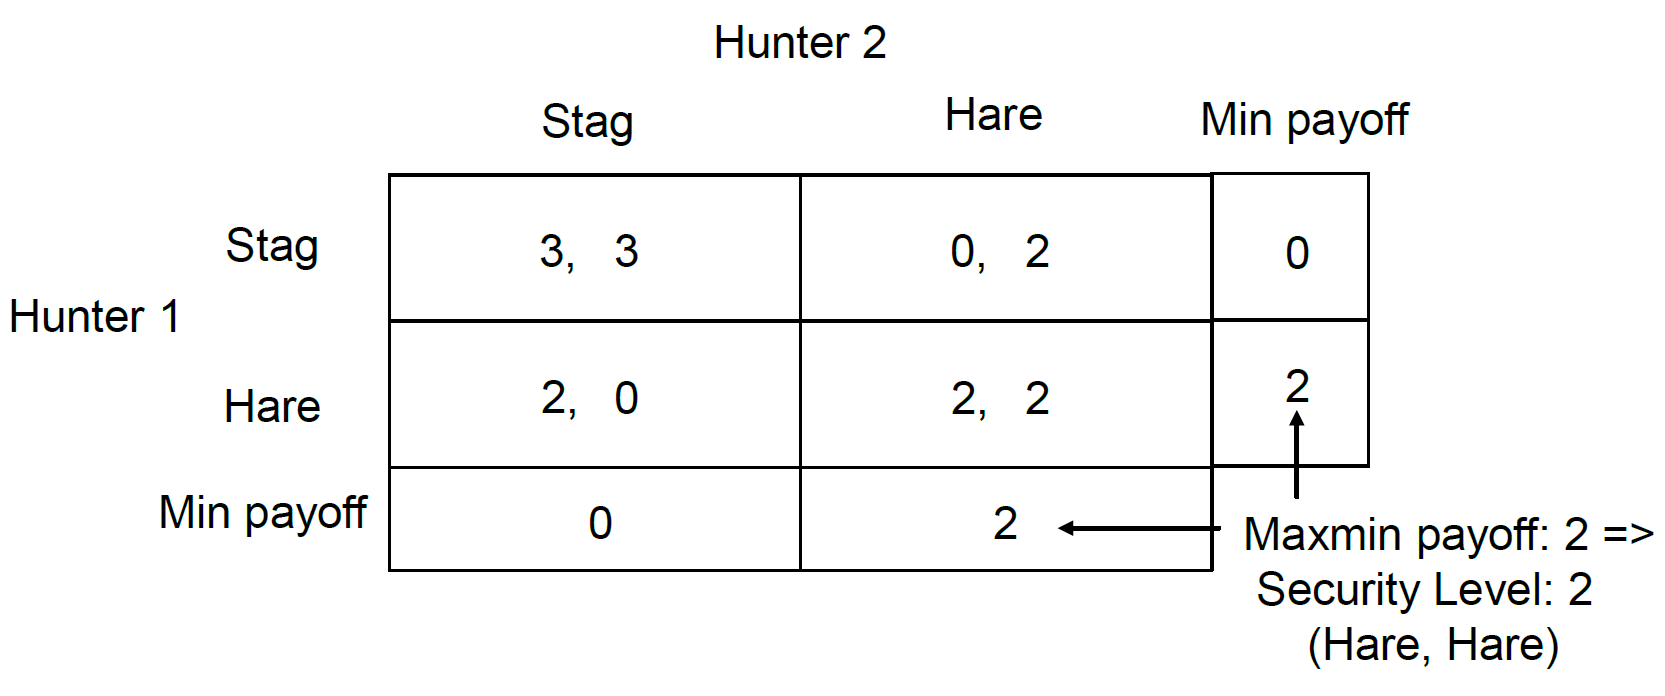
\includegraphics[width=0.5\textwidth]{Pictures/hunter_security_risk_analysis.png}
    \caption{Security Risk analysis}
\end{figure}

\begin{figure}[H]
    \centering
    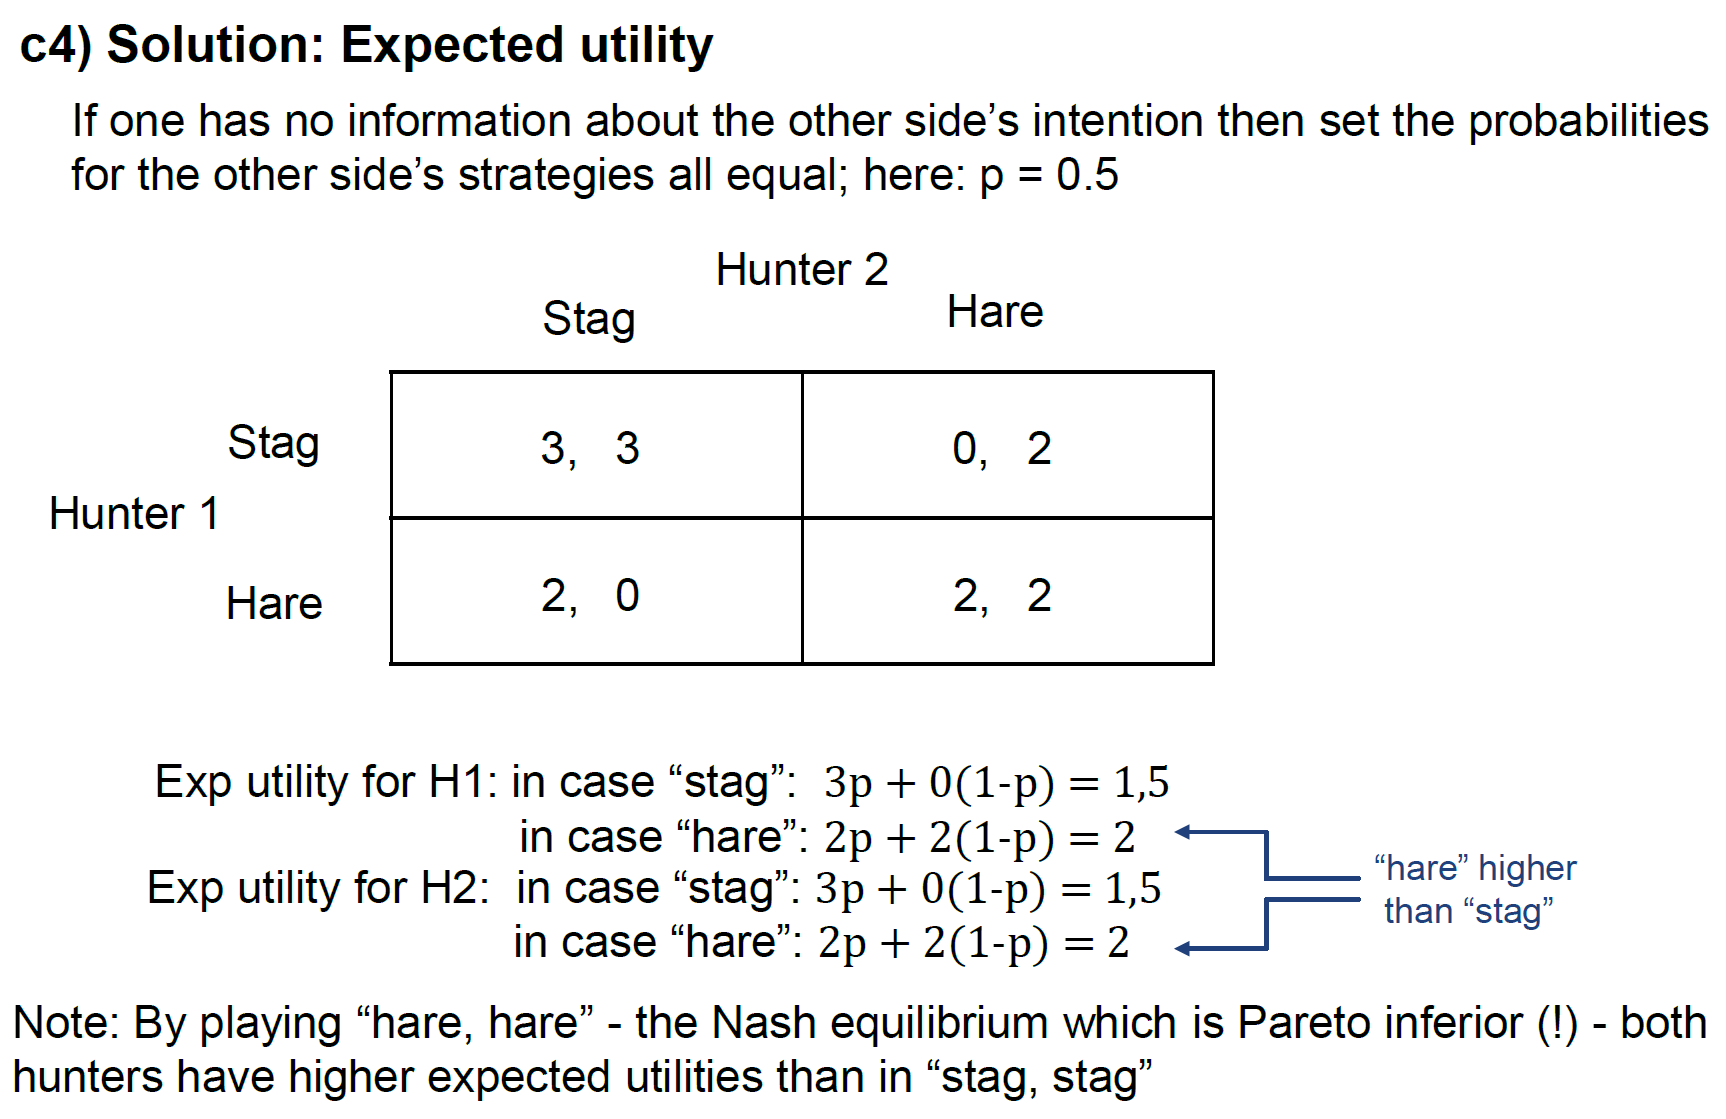
\includegraphics[width=0.5\textwidth]{Pictures/hunter_expected_utility.png}
    \caption{Expected Utility}
\end{figure}

\begin{figure}[H]
    \centering
    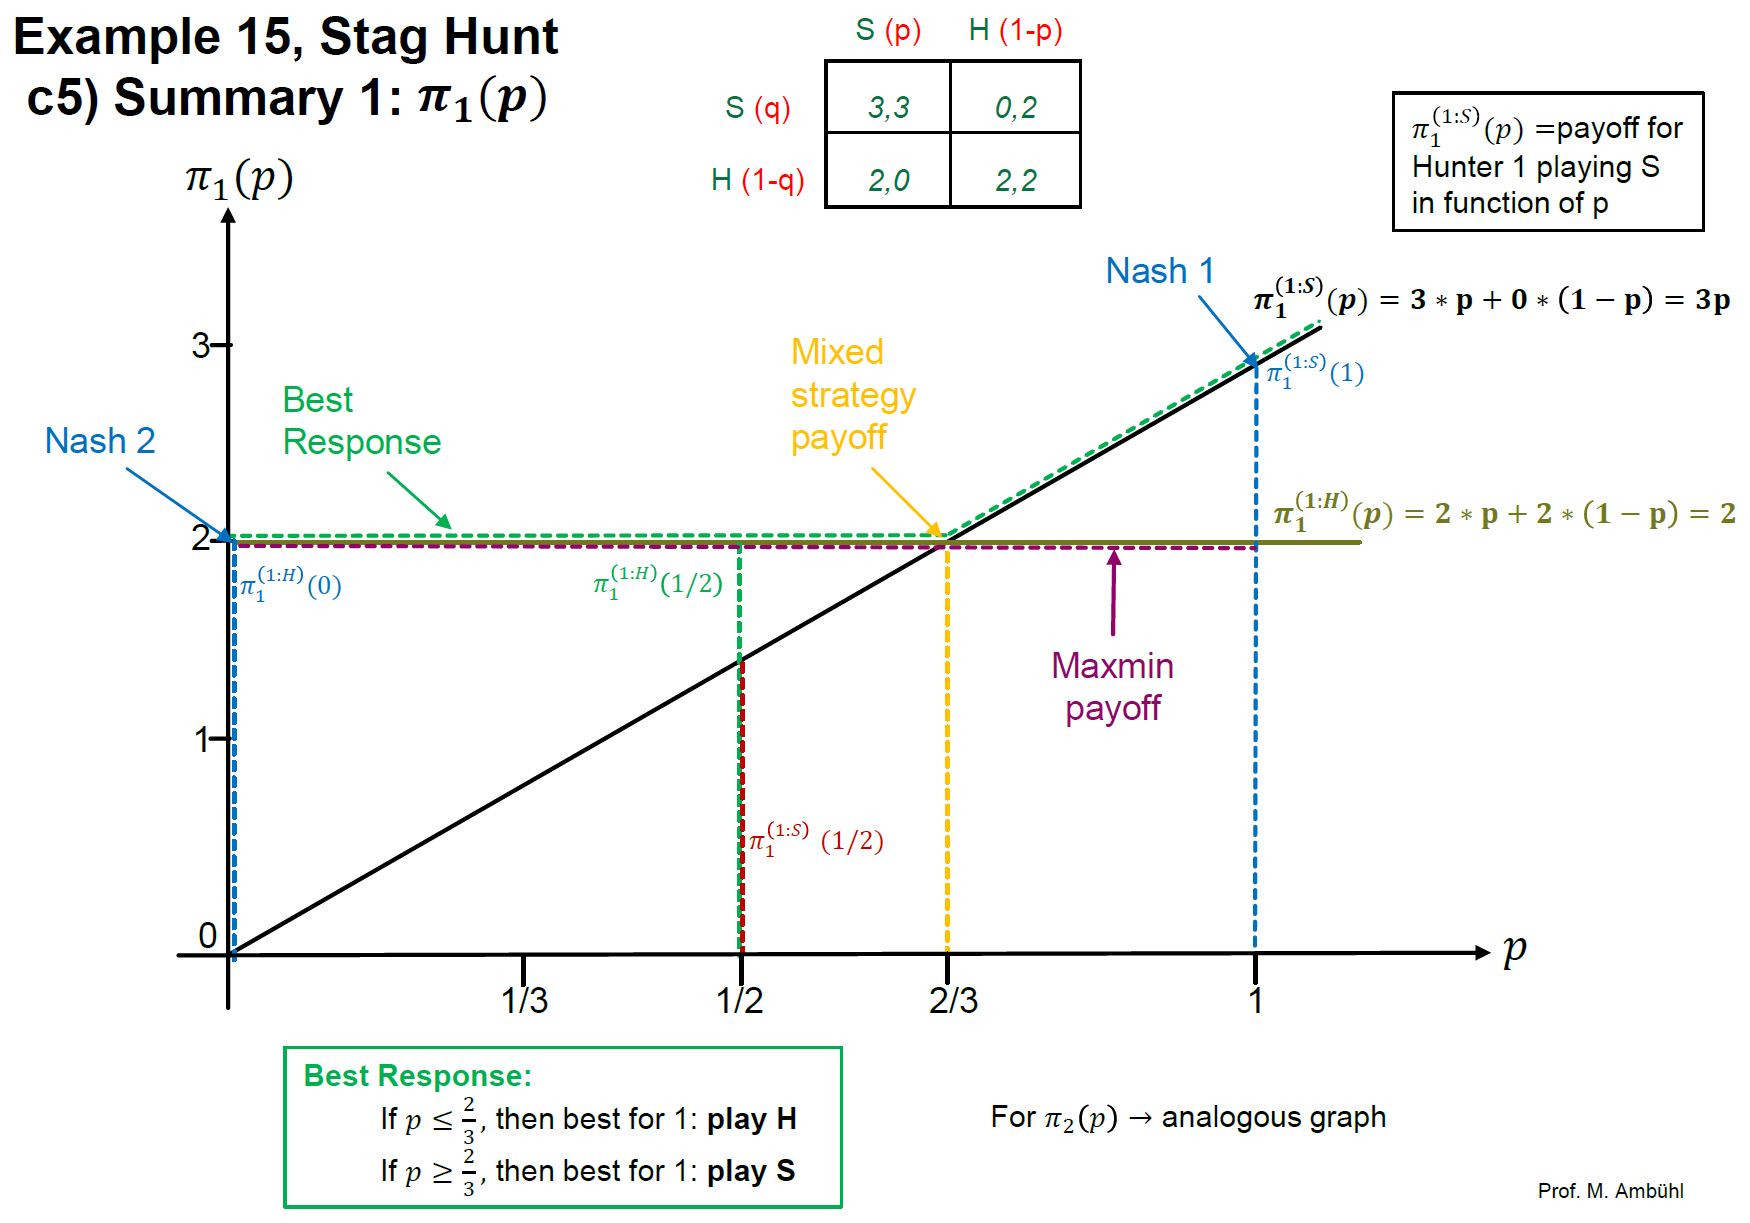
\includegraphics[width=0.5\textwidth]{Pictures/stag_hunt_summary.png}
    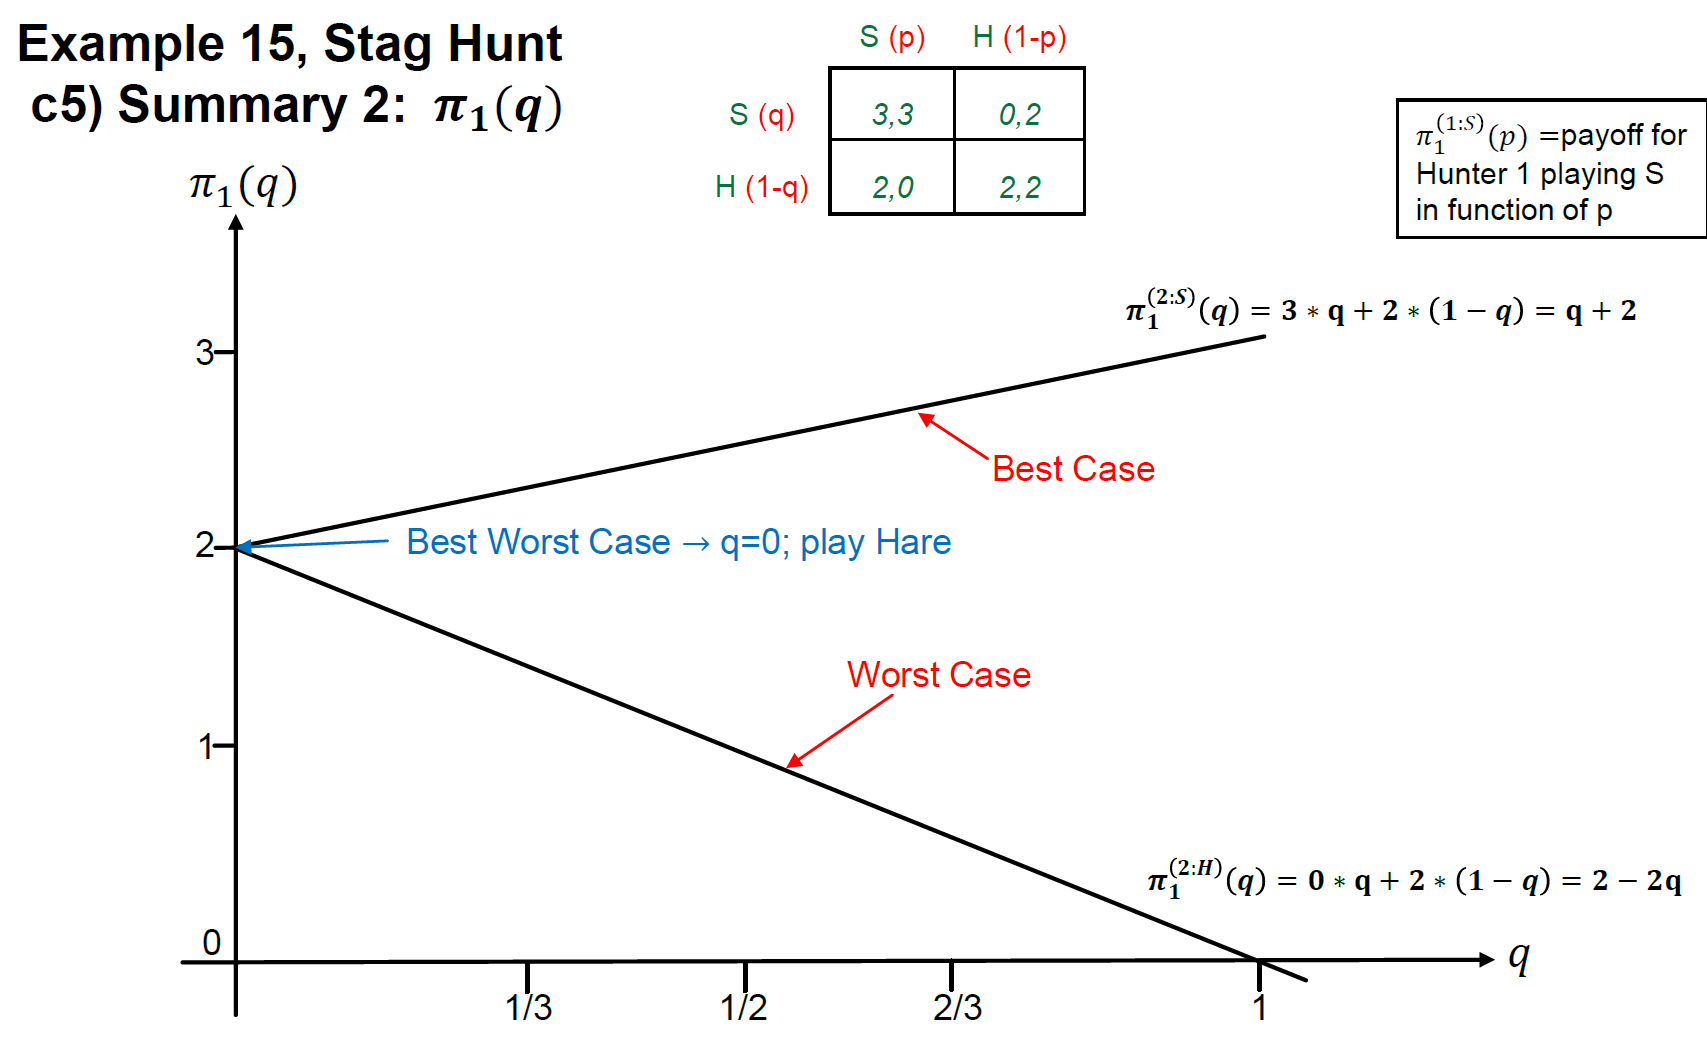
\includegraphics[width=0.5\textwidth]{Pictures/stag_hunt_summary_2.png}
    \caption{Stag Hunt summary}
\end{figure}

\underline{Example 16: 'Arms race' game}
Situation:
\begin{itemize}
    \item Arms race is the process of excessive investment in weapons, military
        technology and the army. Prominent examples:
        \begin{itemize}
            \item Great Britain and Germany competed on having the best navy
                before WW\uproman{1}
            \item Nuclear arms race between the US and the SU
        \end{itemize}
    \item Generally the arms race can be characterized by a country's desire to
        have a military advantage, whenever the counterparty does not arm.
        Staying ahead in military terms allows a country to maintain a
        powerful position.
    \item Whenever all countries are well armed, no one has an advantage,
        but the excessive investment may even hurt the economies.
\end{itemize}

Game:
\begin{enumerate}[(i)]
    \item Players: 3
    \item Actions of players: Arm, Disarm
    \item Payoffs are presented in th enormal form below.
\end{enumerate}

\begin{figure}[H]
    \centering
    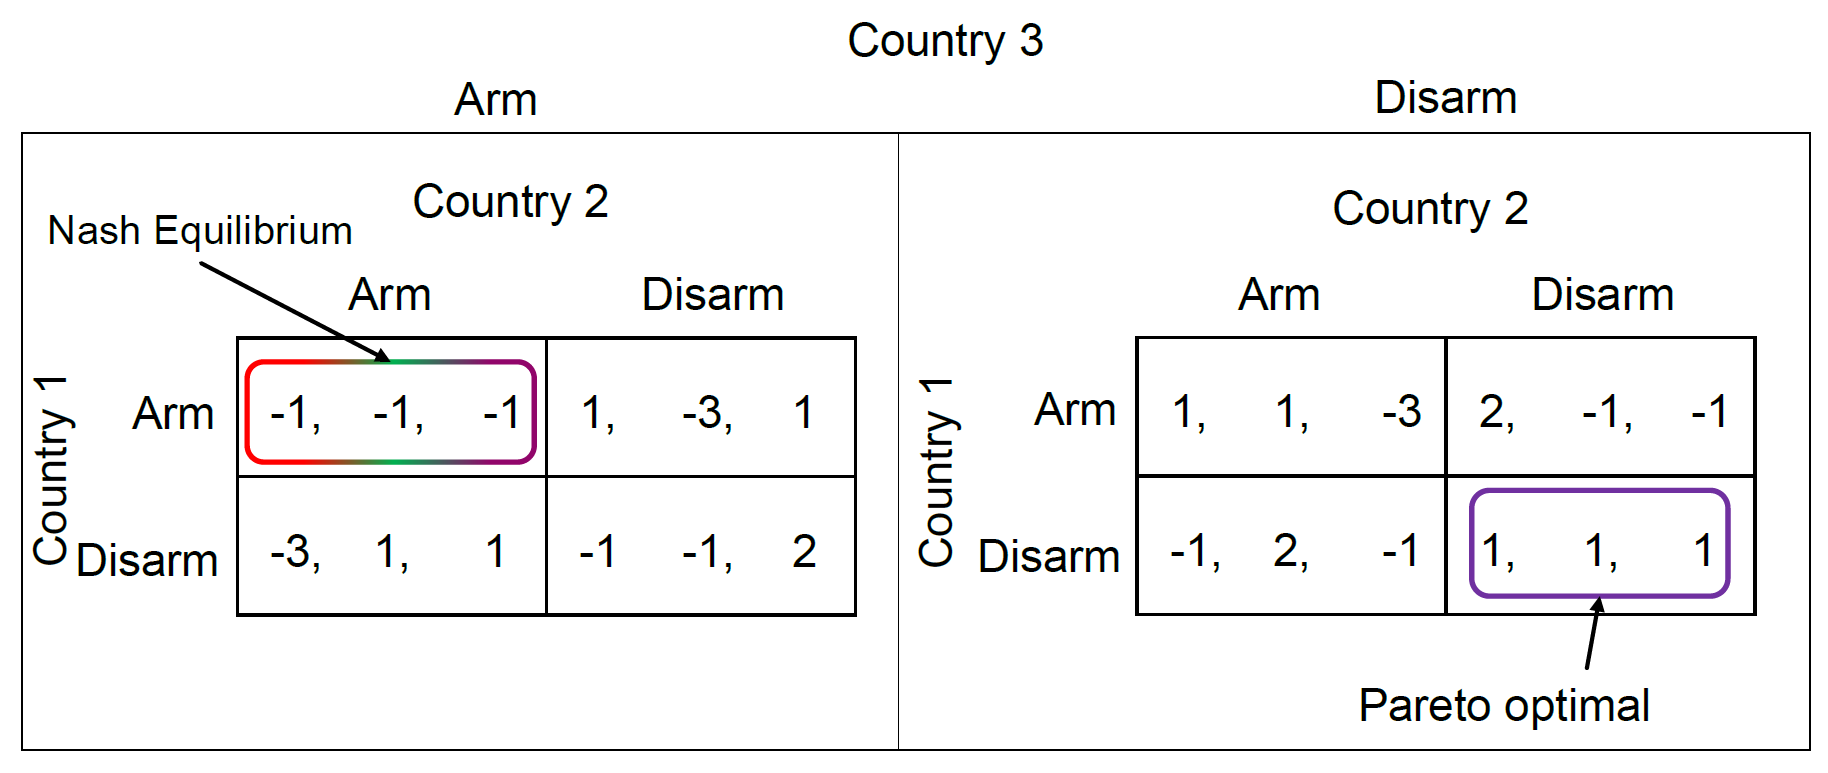
\includegraphics[width=0.6\textwidth]{Pictures/arms_race_nash_equilibrium.png}
\end{figure}

Comments:
\begin{itemize}
    \item Example $16$ illustrates the "non-cooperative simultaneous move"
        game in the normal form in case of $3$ players.
    \item Arms race is another example of the Prisoners' Dilemma: Every country
        is better off when no one increases their military capabilities, but this
        cooperative outcome is not sustainable as a Nash Equilibrium.
\end{itemize}

\vspace{1\baselineskip}

\underline{Example: Turkey Greece refugee question}

\begin{figure}[H]
    \centering
    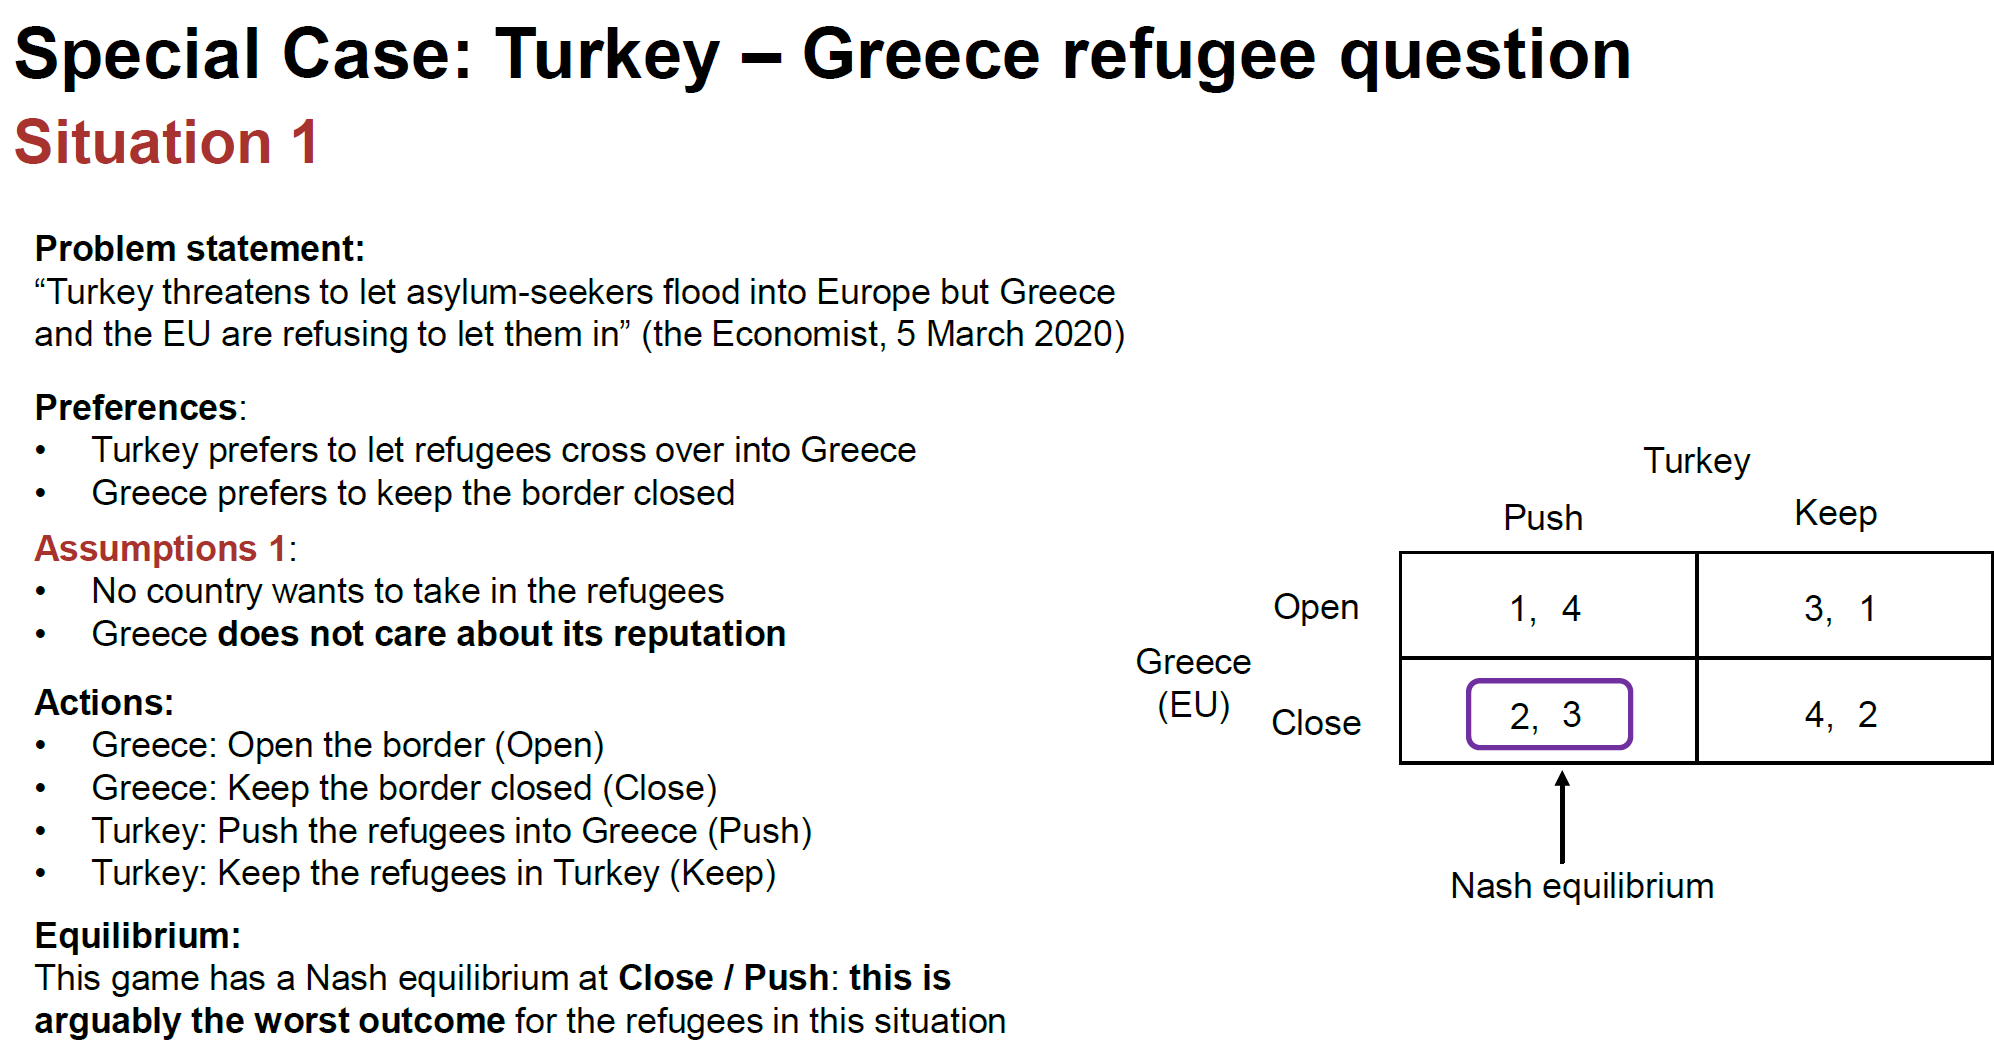
\includegraphics[width=0.8\textwidth]{Pictures/turkey_greece_refugees.png}

    \vspace{1\baselineskip}

    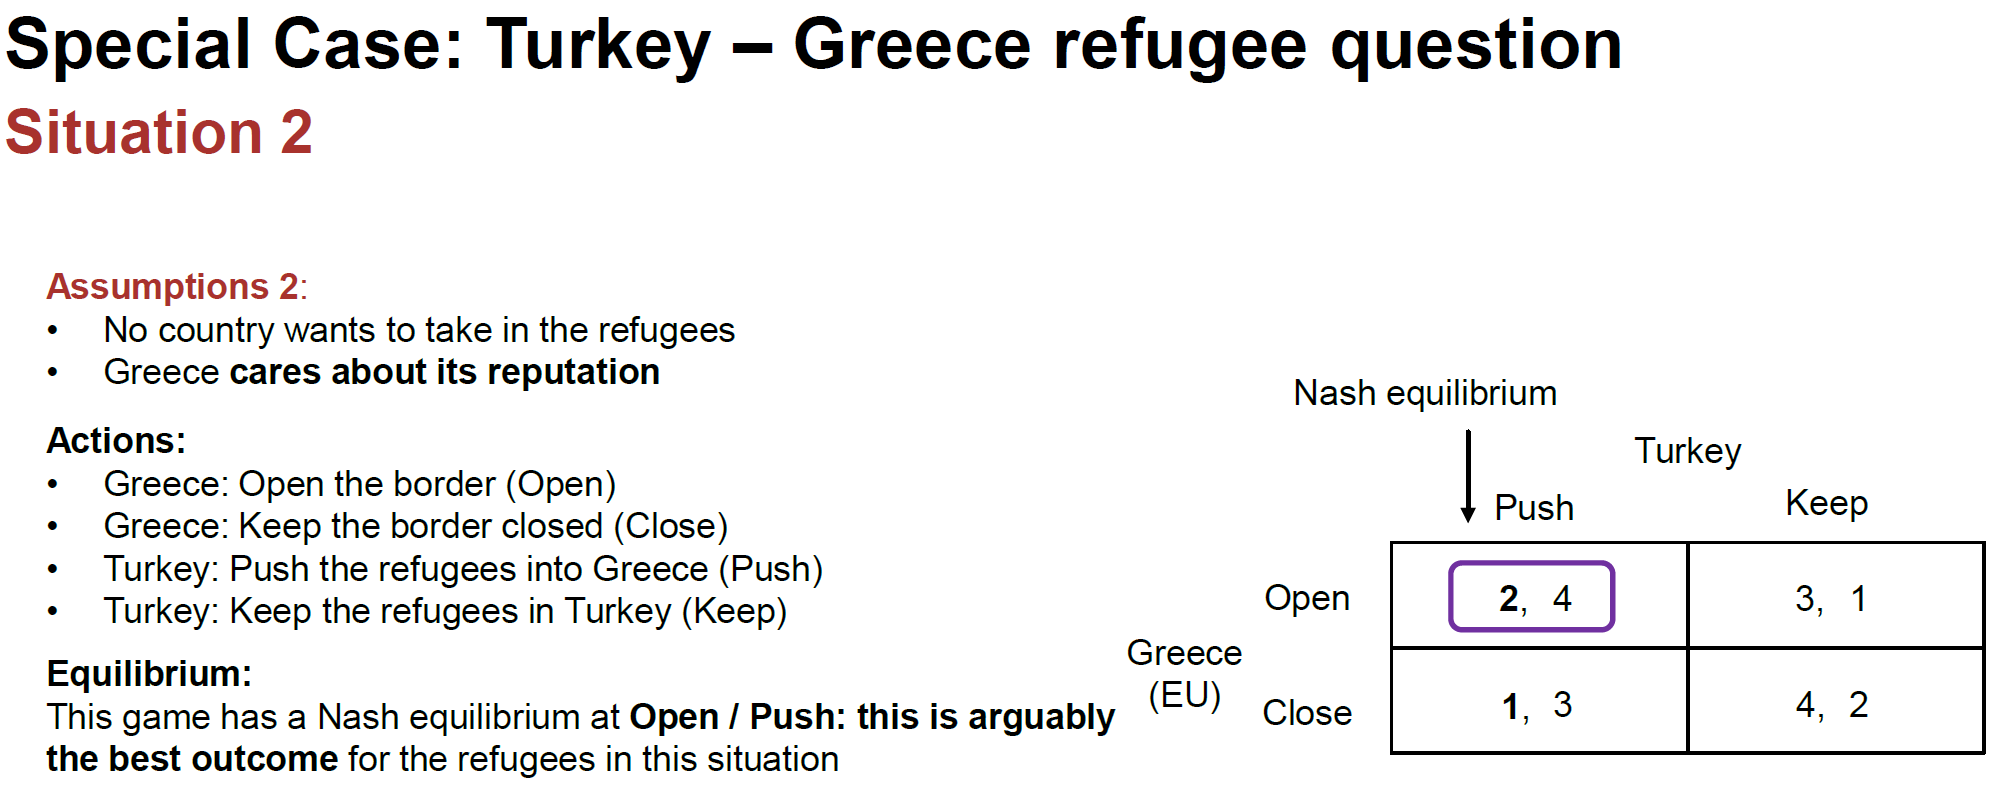
\includegraphics[width=0.8\textwidth]{Pictures/turkey_greece_refugees_2.png}
\end{figure}

\underline{Example}

\vspace{1\baselineskip}

17 Camels should be distributed to $3$ children according to the following
distribution:
\begin{itemize}
    \item $\frac{1}{2}$ goes to the oldest son
    \item $\frac{1}{3}$ goes to the middle son
    \item $\frac{1}{9}$ goes to the youngest son
\end{itemize}

\begin{figure}[h]
    \centering
    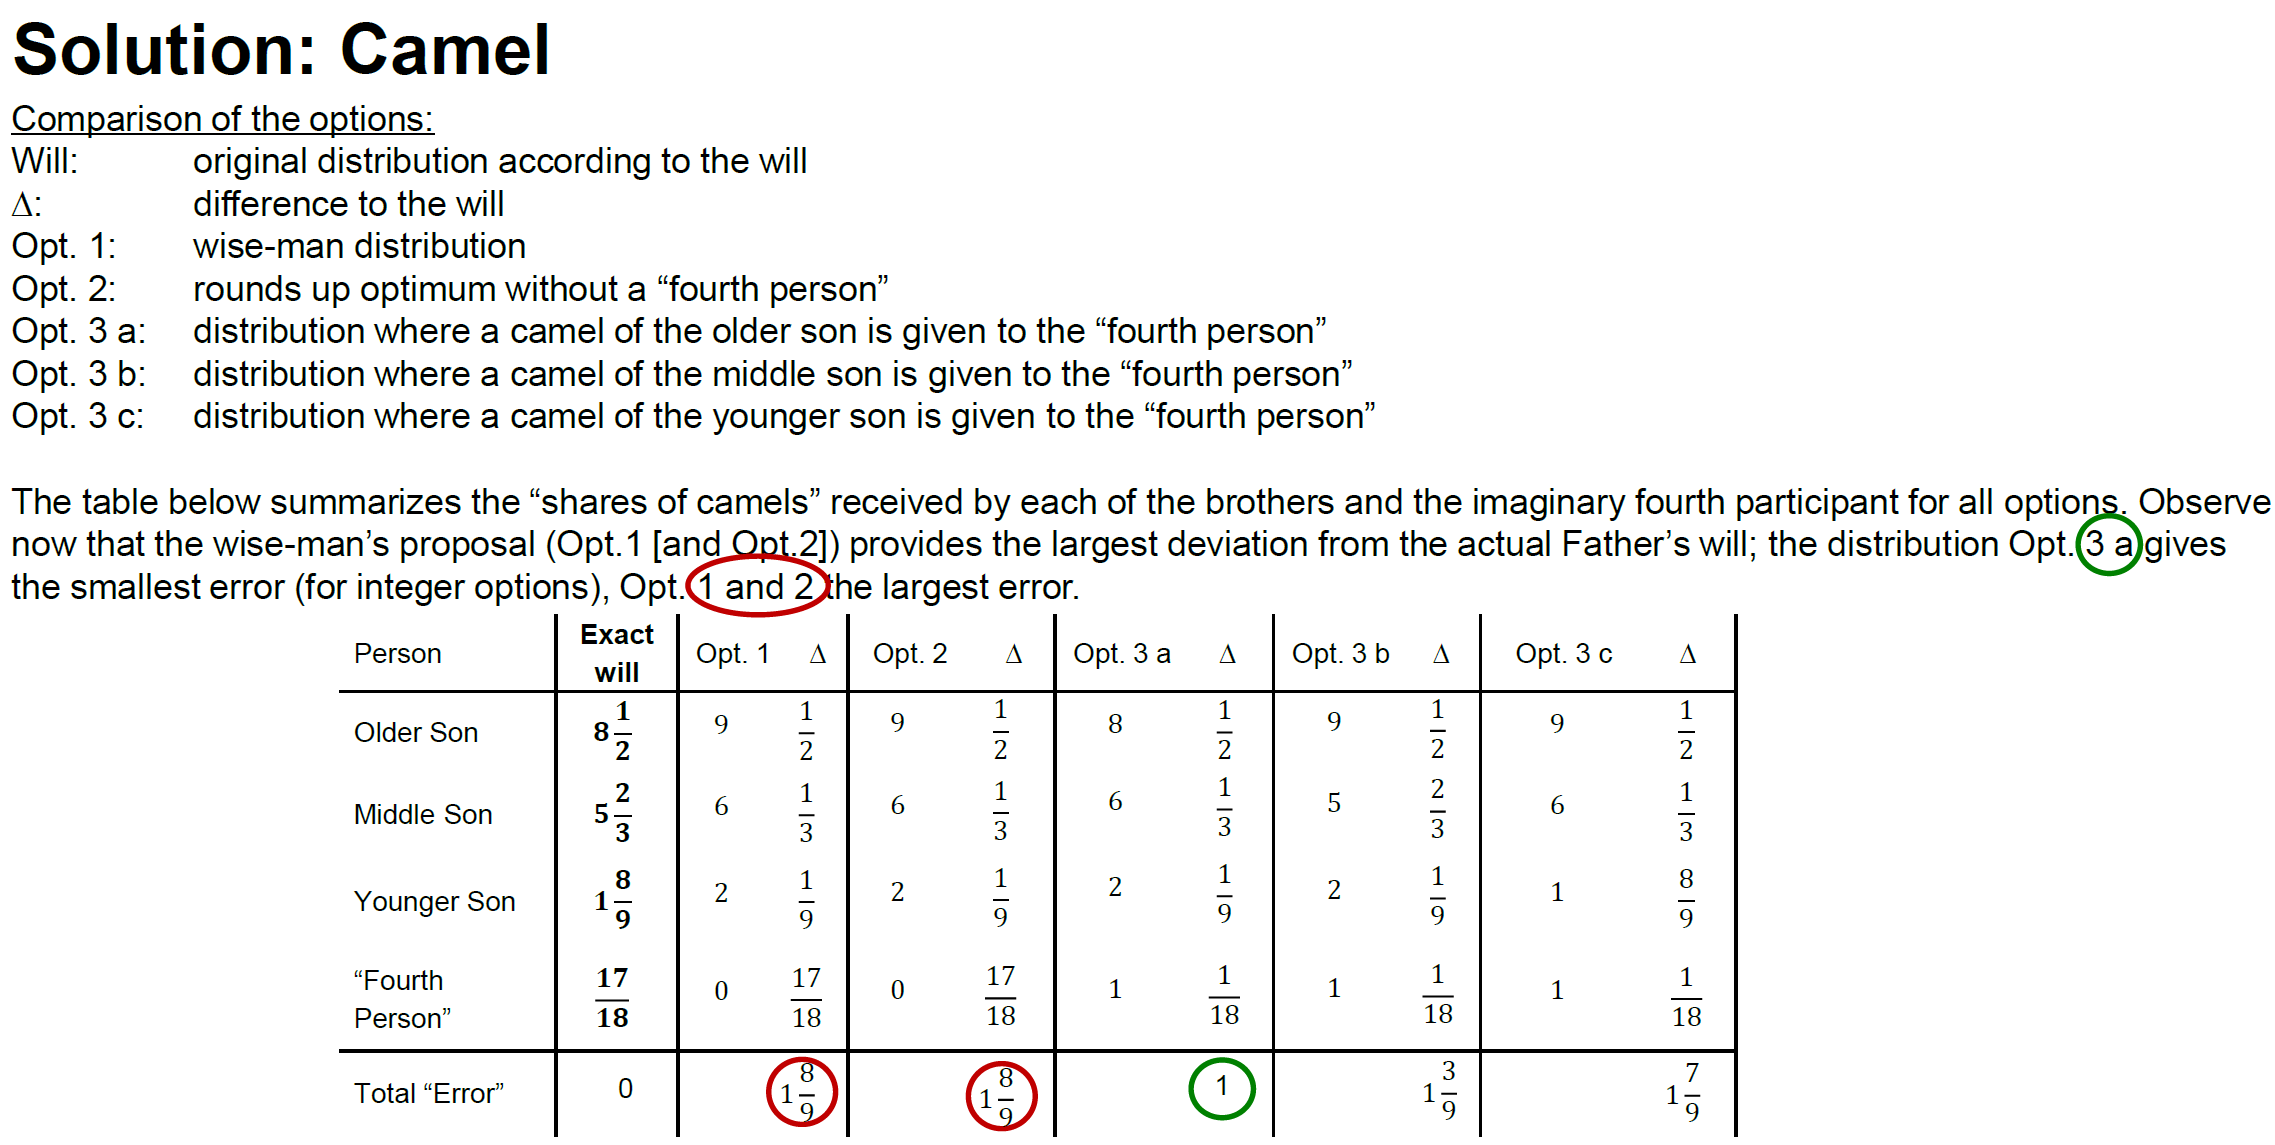
\includegraphics[width=0.9\textwidth]{Pictures/Camel_solutions.png}
    \caption{Solution to the Camel problem}
\end{figure}


\paragraph{Dynamic Games}

\begin{itemize}
    \item Contrary to a static game, in a dynamic game players take action
        over time.
    \item A static game can be seen as one 'one-shot' game, whereas in a dynamic
        game a player can move more than once.
    \item We will consider dynamic games of perfect information, i.e. games in
        which each player, when taking an action, is perfectly informed of all
        the events that have previously occured.
\end{itemize}

\subparagraph{Sequential move games}

\begin{itemize}
    \item In sequential move games players have some knowledge about earlier
        actions of the game, i.e. decisionmaking happens sequentially - one
        player takes his action before the other does.
\end{itemize}

\vspace{1\baselineskip}

\underline{Example 17: 'Nuclear deterrence' game}

\begin{enumerate}[a)]
    \item Situation in words:
        \begin{itemize}
            \item During the Cold War, the US and SU had big nuclear
                arsenals and neither side could 'disarm' the other side with
                just the first nuclear strike - each side secured second strike
                capabilities - both could have responded to any nuclear strike
                with a devastating retaliatory strike (e.g. from submarines)
            \item Knowing this, consider now the situation where one country
                decides first whether to launch an attack or to delay it. In case
                it delays an attack, the second country can make its own decision
                whether to attack or not.
            \item When both countries delay an attack, the status quo is preserved
            \item Whenever there is an attack, both aggressor and defender suffer
                from the nuclear war, however there is a slight first-mover advantage
                in comparison to the defender.
        \end{itemize}
    \item Game
        \begin{enumerate}[(i)]
            \item Players: 2
            \item Strategies of players: Attack, Delay
            \item Sequence of moves is shown in the extensive form game
                (e.g. in the game tree)
            \item Payoffs are given in the terminal nodes (i.e. places where the game
                tree ends).
        \end{enumerate}
        \begin{figure}[H]
            \centering
            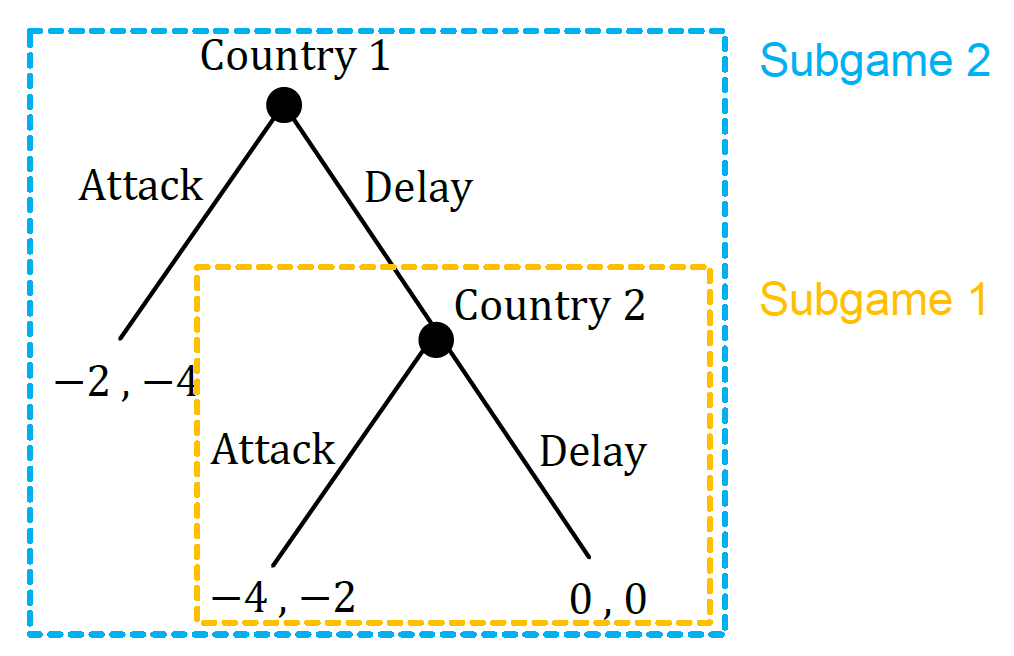
\includegraphics[width=0.5\textwidth]{Pictures/nuclear_example_1.png}
        \end{figure}
    \item Solution
        \begin{enumerate}[c1)]
            \item Some definitions:
                \begin{enumerate}[(1)]
                    \item A subgame is a part (sub-tree) of a game that satisfies
                        the following conditions:

                        a) It begins at a decision node (for any player)

                        b) The player knows all the decisions that have been
                            made up until that time

                        c) The sub-tree contains all the decision nodes that
                            follow the initial node (and no other)
                            
                        Example: There are two subgames in Example 17
                    \item A strategy is a rule for choosing an action at every point
                        that a decision might have to be taken by the player. A strategy
                        is a complete plan of actions.
                \end{enumerate}
            \item Backwards Induction and Subgame Perfect Nash Equilibrium
                \begin{itemize}
                    \item The most common way of solving dynamic games is through
                        backwards induction. In this procedure, the last player
                        to act at each node chooses the action that maximizes
                        his utility (i.e. the Nash Equilibrium)

                        The second to last player then chooses his action optimally,
                        knowing that the last player chooses optimal actions at each
                        node. This process continues until each player has chosen
                        optimally under the assumption that all future players
                        make optimal choices.
                    \item Applying backwards induction always results in a pure
                        strategy Nash Equilibrium (i.e. there is always at least
                        one Nash Equilibrium in pure strategy)
                    \item The resulting equilibrium is called a \textit{Subgame
                        Perfect Nash Equilibrium} as it induces a Nash Equilibrium
                        in every subgame of the whole game.
                    \item The concept of subgame perfection was formulated by Reinhard
                        Selten.
                \end{itemize}
            \item Solution to example 17:
                
                In Subgame Perfect Nash Equilibrium both countries decide to delay.
        \end{enumerate}
    \item Comments:
        \begin{itemize}
            \item This model assumes the order of moves: First is Country $1$
                and second is country $2$. (In reality, however, both countries
                can pretend to be the first to move and both countries can be
                unsure whether delaying a move will transition to the status quo
                or give the other side the opportunity to launch its own strike.)
                
                $\rightarrow$ More elaborate games (e.g. game with imperfect
                information) may be better suited for analysis.
            \item Subgame Perfect Nash Equilibrium is a more suitable solution
                concept for dynamic games than just Nash Equilibrium - it rules
                out some 'unrealistic' Nash Equilibrium predictions (see Exercise
                Session)
        \end{itemize}
\end{enumerate}

\vspace{1\baselineskip}

\underline{Example 18: 'Political crisis' game}

\begin{enumerate}[a)]
    \item Situation:
        \begin{itemize}
            \item In a country there is a conflict between the government and
                the opposition.
            \item The Government has now the choice between proposing a broad
                package of reforms or escalating the conflict by calling in the
                army
            \item In case the reforms are proposed, the opposition can decide
                whether to accept them or to continue the protests.
            \item In case the military option is chosen, the opposition
                decision is reduced to either giving-in or resisting.
        \end{itemize}
    \item Game:
        \begin{enumerate}[(i)]
            \item Players: 2
            \item Action of players:
                \begin{itemize}
                    \item Government: Reform, Escalate
                    \item Opposition:
                        \begin{itemize}
                            \item In the case of Reform is chosen: Accept, Reject
                            \item In the case of Escalate is chosen: Give-in, Resist
                        \end{itemize}
                \end{itemize}
            \item Sequence of moves is shown in the extensive form game (e.g. in the game tree)
            \item Payoffs are given in the terminal nodes.
            \begin{figure}[H]
                \centering
                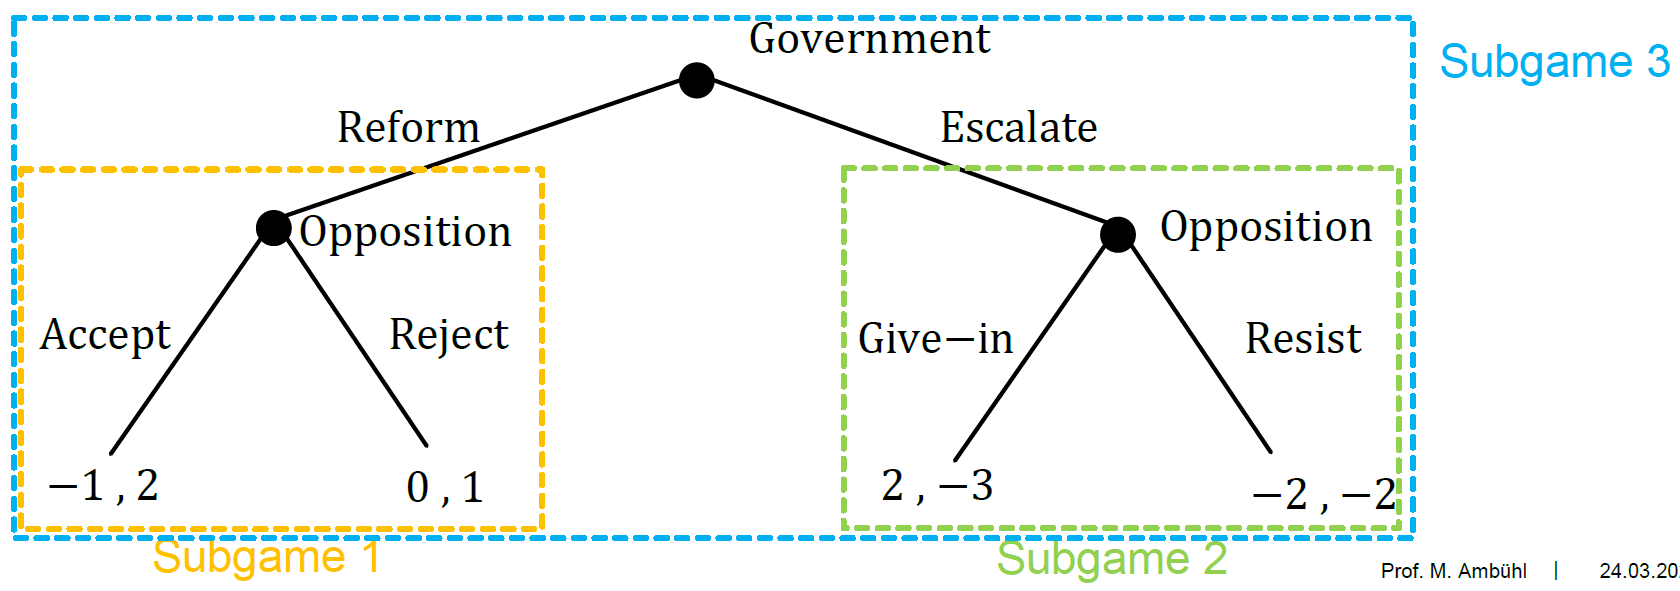
\includegraphics[width=0.7\textwidth]{Pictures/political_crisis_example.png}
            \end{figure}
        \end{enumerate}
    \item Solution:
    
        Subgame Perfect Nash Equilibrium:
        \begin{itemize}
            \item Government: Plays Reform strategy (Because, if they play
                Escalate, the opposition will play Resist)
            \item Opposition: Plays Accept, if Reform is observed and plays
                Resist, if Escalation is observed from the government side
        \end{itemize}
    \item Comment
        \begin{itemize}
            \item Example 18 illustrates the concept of a strategy in a dynamic
                game. A strategy is a complete list of actions. Thus it prescribes
                an optimal action even in the decision nodes, which are not reached
                by the equilibrium play of the game.
        \end{itemize}
\end{enumerate}

\subparagraph{Repeated simultaneous move games}

A repeated game consists of some number of iterations of a simultaneous move game
(i.e. the stage game). A repeated game can be either finite (i.e. with a finite
number of repetitions) or infinite (e.g. without a time horizon).

\vspace{1\baselineskip}

\underline{Example 19: 'Infinite interactions' game}

\begin{enumerate}[a)]
    \item Situation:
        \begin{itemize}
            \item Recall: In Example 13 the Nash Equilibrium was when both
                sellers chose low prices. However, if both choose high prices,
                both will win. (See Example 13)
            \item In reality, competing sellers meet each other every day, i.e.
                they play the game from Example 13 many times in a row, possibly
                an infinite amount of times.
            \item Can the Pareto efficient outcome be achieved, if the game
                is repeated infinitely many times?
        \end{itemize}
    \item Game:
        \begin{enumerate}[(i)]
            \item Players: 2
            \item Actions of players in each stage of the game: high, low
            \item Discounted Payoffs:
                \begin{itemize}
                    \item Each seller discounts his future payoff - discount factor $0 < \delta < 1$
                    \item Total payoff to player $i$ is $\sum_{t=0}^\infty \delta^t \cdot r_i(t)$
                        where $r_i(t)$ is a payoff received in stage $t$.
                \end{itemize}
        \end{enumerate}
    \item Solution
        \begin{enumerate}[c1)]
            \item Concept:
                \begin{itemize}
                    \item In every stage of the game players can choose an
                        action: High or Low price
                    \item There are several tactics that players should play
                        depending on the history of the game. One of them is the
                        so called "Grim Trigger" strategy. This strategy is
                        specified as follows:
                        \begin{itemize}
                            \item start by setting High price (i.e. cooperate with the other player)
                            \item continue with High price until either player sets Low price
                                (i.e. until you or him defect)
                            \item then set Low price forever.
                        \end{itemize}
                \end{itemize}
            \item Solution to Example 19:
                \begin{itemize}
                    \item Suppose Seller $2$ sticks to the Grim Trigger strategy,
                        then if Seller $1$ sets the High Price, it will establish
                        a cooperation in the long run. This generates flow of
                        utility $\sum_{t=0}^\infty \delta^t \cdot 300 = \frac{300}{1-\delta}$
                    \item Suppose now Seller $1$ decides to deviate in the first stage and sets the
                        low price (which brings him an immediate return of $500$). According to
                        the Grim Trigger strategy, Seller $2$ will set the low price in the next
                        round. This generates flow of utility:
                        $500 + \sum_{t=1}^\infty \delta^t \cdot 250 = 500 + \frac{250 \cdot \delta}{1 - \delta}$
                    \item Neither of the sellers will find it profitable to deviate if:
                        $\frac{300}{1 - \delta} > 500 + \frac{250 \cdot \delta}{1 - \delta}$,
                        or $\delta > \frac{200}{250} =  0.8$
                \end{itemize}
        \end{enumerate}
\end{enumerate}

\vspace{1\baselineskip}

\underline{Example 20: Repeated Prisoners' Dilemma}

There are other strategies which achieve cooperation; one of the most successful
strategies in experiments was "Tit-fot-Tat".

\begin{itemize}
    \item In negotiation you often have multiple phases/rounds.
    \item "Tit for Tat" strategy ("As you to unto me, so I do unto you") is
        a famous strategy (in game theory) for repeated games, developed by
        Anatol Rapoport for an experiment by Robert Axelrod:
        \begin{itemize}
            \item begin by playing cooperatively
            \item then do whatever the other player did in the last stage
        \end{itemize}
    \item "Tit for Tat" is a remarkably good and robust strategy for playing
        iterated Prisoner's Dilemma.
    \item Such s strategy should follow these principles:
        \begin{itemize}
            \item Nice: Start by cooperating, and never be the first to defect
            \item Retaliation: Reliably punish defection by the opponent
            \item Forgiving: If you punish defection, be willing to try to
                cooperate again.
            \item Clear: The pattern should be consistent and easy to predict
                (by the opponent)
        \end{itemize}
    \item Is is a cooperation strategy of "friendly reciprocity"
\end{itemize}

\subsubsection{Cooperative Games}

\paragraph{Introduction}

Concept: Players talk to each other to decide on a reasonable or fair outcome
and agree to implement the decision.

\subparagraph{Example 21: 'Rose and Colin' game}

\begin{enumerate}[a)]
    \item Game
        \begin{enumerate}[(i)]
            \item Players: 2
            \item Action of players: $A,B$
            \item Payoffs: Preferences are summarized in the normal form below:
            \begin{figure}[H]
                \centering
                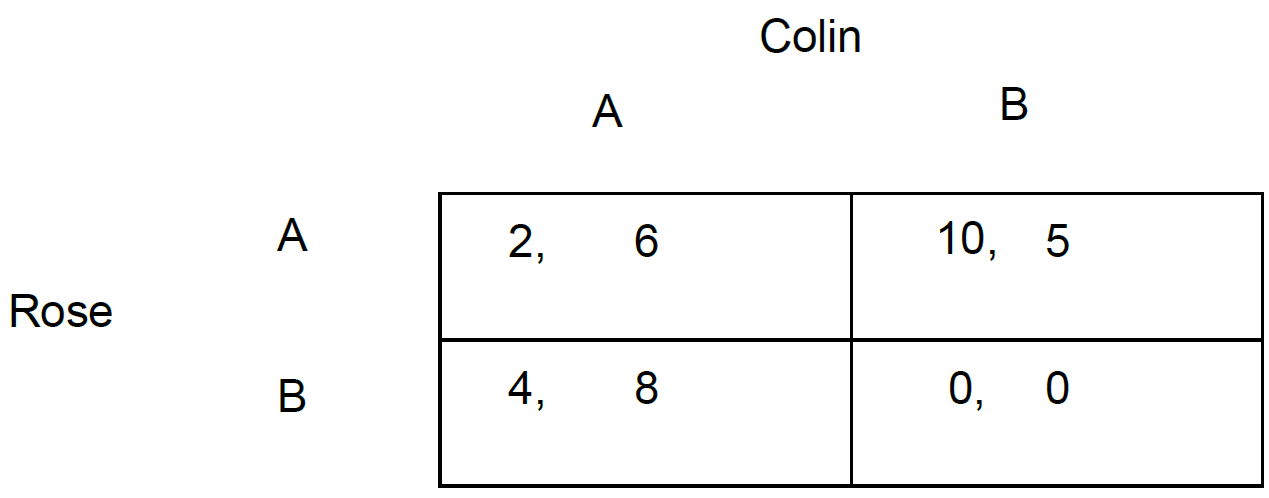
\includegraphics[width=0.5\textwidth]{Pictures/rose_colin_example.png}
            \end{figure}
        \end{enumerate}
    \item Solution
        \begin{enumerate}[b1)]
            \item Non-cooperative approach:
                Nash Equilibrium in the bottom left corner. Observe:
                Colin has a dominant strategy $A$. This strategy guarantees
                him a payoff of $6$.
            \item Security levels:
                Secirity strategy is the strategy which guarantees the minimum
                payoff for a player, when he plays non-cooperatively.
                \begin{itemize}
                    \item Colin's security level:
                        Recall, Colin has a dominant strategy - strategy $A$;
                        it guarantees him a security level payoff $\pi_C^{sec} = 6$
                    \item Rose's security level:
                        Suppose Rose plays $A$ with probability $q$ and $B$ with
                        $(1-q)$. Her expected payoffs are:
                        \begin{itemize}
                            \item If Colin plays $A$: $q \cdot 2 + (1-q) \cdot 4$
                            \item If Colin plays $B$: $q \cdot 10 + (1-q) \cdot 0$
                        \end{itemize}
                        We obtain her maximum strategy $q^{sec} = \frac{1}{3}$.
                        This gives her a security level payoff
                        $\pi_R^{sec} = q^{sec} \cdot 2 + (1-q^{sec}) \cdot 4 = \frac{10}{3}$
                \end{itemize}
                \begin{figure}[H]
                    \centering
                    \includegraphics[width=0.6\textwidth]{Pictures/rose_colin_payoff.png}
                \end{figure}
            \item Payoff Polygon:
                \begin{figure}[H]
                    \centering
                    \includegraphics[width=0.7\textwidth]{Pictures/rose_colin_payoff_polygon.png}
                \end{figure}
                Question: What would be a fair outcome for Rose and Colin?
                Could we choose, within the range of the negotiation set, a single
                outcome as the fairest?
        \end{enumerate}
\end{enumerate}

\paragraph{Nash axioms for a fair outcome}

\begin{enumerate}[]
    \item AXIOM 1: Rationality - the solution point should be in the negotiation set
    \item AXOIM 2: Linear invariance - if either Rose's or Colin's payoffs are transformed
        by a positive linear function, the solution point should be transformed by
        the same function.
    \item AXIOM 3: Symmetry - if the polygon happens to be symmetric about the line
        of slope $+1$ through $SQ$, then the solution point should be on this line.
    \item AXIOM 4: Independence of irrelevant alternatives - suppose NBS is the
        solution point for a polygon $P$ with status quo point $SQ$. Suppose $Q$
        is another polygon which contains both $SQ$ and $NBS$, and is totally
        contained in $P$. Then $NBS$ should also be the solution point for $Q$
        with status quo $SQ$.
\end{enumerate}

\subparagraph{Nash Bargaining Solutions (NBS)}

There is a one and only arbitrary scheme which satisfies Axioms 1-4.
\begin{itemize}
    \item if $SQ = (\pi_R^{sec},\pi_C^{sec})$, then arbitrated solution point
        NBS is the point $(\pi_R,\pi_C)$ in the polygon with $\pi_R \geq \pi_R^{\sec}$,
        $\pi_C \geq \pi_C^{\sec}$
    \item which maximizes the product: $(\pi_R - \pi_R^{\sec}) \cdot (\pi_C - \pi_C^{sec})$
\end{itemize}
Meaning, for our problem, we need to solve
\begin{align*}
    \max_{\pi_R , \pi_C} \geschwungeneklammer{\klammer{\pi_R - \frac{10}{3}} \cdot \klammer{\pi_C - 6}}
\end{align*}
subject to
\begin{align*}
    \pi_C &= - \frac{1}{2} \pi_R + 10 \hspace{10pt} \text{(equation for negotiation set line)}
    \\
    \pi_R &\geq \frac{10}{3}
    \\
    \pi_C &\geq 6
\end{align*}
\begin{figure}[H]
    \centering
    \includegraphics[width=0.5\textwidth]{Pictures/rose_colin_payoff_polygon_NBS.png}
\end{figure}

\paragraph{Threats and alternations of $SQ2$}
\begin{itemize}
    \item Players may try to influence the outcome of the NBS by using threat
        strategies, e.g.: "If negotiations breaks down, I will pay the following
        strategy, which will be bad for you!" In our example: "I will play $A$
        if the negotiations break down."
    \item By doing this, Colin would only get $6$ (playing $A$) instead of $8$.
    \item However, Rose would have lowered her $SQ$ from $\pi_R^{sec} = 3 \frac{1}{3}$
        to $\pi_R^{sec} = 2$
    \item What would happen?
\end{itemize}
\begin{figure}[H]
    \centering
    \includegraphics[width=0.6\textwidth]{Pictures/rose_colin_new_SQpng.png}
\end{figure}

\vspace{1\baselineskip}

\paragraph{Dealing with threats in negotiation}

Strategies that are likely to fail:
\begin{itemize}
    \item \underline{Striking a direct counterattack}: your threats may not
        be sufficiently credible or could launch an uncontrollable conflict excalation
        \begin{itemize}
            \item However, in situations where your aggressor only responds to
                aggression, a counterattack can establish your credibility. In such
                situations, issue a reasonable counter threat and then immediately
                proceed to identify each other's interests to prevent conflict
                escalation
        \end{itemize}
    \item \underline{Concede immediately}: that would reinforce his/her domineering
        tactics.
\end{itemize}

\subparagraph{DEAL approach offered by the Harvard Program on Negotiations}

\begin{enumerate}
    \item Diagnose the threat:
        \begin{itemize}
            \item Remove yourself from the situation: physically and pychologically
            \item Consider the motivation behind the threat $>$ to determine your response:
                \begin{itemize}
                    \item \underline{The victim}: your counterpart is feeling frustrated or offended,
                        the threat might have emerged from his/her need to be acknowledged
                    \item \underline{The pragmatists}: your counterpart is straight forward, the threat
                        is informing you of his/her real constraints or strong outside
                        alternatives.
                    \item \underline{The bluffer}: your counterpart is feeling insecure, the threat is
                        rather a trick
                \end{itemize}
        \end{itemize}
    \item Express understanding
        \begin{itemize}
            \item Listen to your counterparts grievances and acknowledge them,
                but be careful not to offer concessions to $>$ to help reduce tension
                and further threats.
        \end{itemize}
    \item Ask questions
        \begin{itemize}
            \item Ask questions about the needs and alternatives of the counterparty
            to find new solutions to his/her concerns, rather than giving in to
            surface demands $>$ to determine if ZOPA exists and find solutions that
            are better than BATNA for both.
        \end{itemize}
    \item Label the Negotiation Threat
        \begin{itemize}
            \item If you think the threat is a bluff, then let your counterparty
                know that $>$ to boost your sense of control in the situation.
        \end{itemize}
\end{enumerate}

\subsection{Summary}

\begin{figure}[H]
    \centering
    \includegraphics[width=\textwidth]{Pictures/Game_Theory_summary.png}
\end{figure}

\begin{figure}[H]
    \centering
    \includegraphics[width=\textwidth]{Pictures/Game_Theory_summary_2.png}
\end{figure}


\paragraph{Important Definitions}


\begin{figure}[H]
    \centering
    \includegraphics[width=\textwidth]{Pictures/Game_Theory_important_definitions.png}
    \caption{Important Definitions in Gametheory}
\end{figure}


\paragraph{Recommendations}

\begin{itemize}
    \item Define the key elements of the game:
        \begin{itemize}
            \item Who are the players?
            \item Which actions and strategies does each player have?
            \item How do the combinations of the strategies played determine the final payoff?
        \end{itemize}
    \item When you don't know what to do - think of maximizing your minimal gain!
    \item Never play a dominated strategy, play the dominate strategy (if such a one exists)
    \item Calculate your and your opponents' best responses!
    \item Think carefully of your threat strategies to push opponents towards cooperation!
\end{itemize}

\paragraph{Benefits and limits of models}

If
\begin{enumerate}[i]
    \item there are at least two players: a player may be an individual,
        but it may also be a more general entity like a company, a nation,
        or even a biological species.
    \item each player has a number of possibilities, i.e. courses
        of action, which he may choose to follow.
    \item The strategy chosen by each player determine the outcome
        of the game.
    \item Payoffs are associated to each possible outcome of the
        game in a collection of numerical payoffs, one to each
        player; these payoffs represent the value of the outcome
        to the different players.
\end{enumerate}
then a game theoretical approach to the problem at hand is possible.


\paragraph{Comments}

\begin{itemize}
    \item Game theory is a powerful tool for the generation of insights
        into problems.
    \item Game theory needs a considerably high level of abstraction -
        in order to allow for sensible propositions; in difficult problems
        the complexity may often not be reduced to a level which would
        allow the use of a game theoretical approach.
    \item Often it is specifically useful for ex post analysis
\end{itemize}

